% Use only LaTeX2e, calling the article.cls class and 12-point type.

\documentclass[12pt]{article}
%\documentclass[12pt]{nature}

\usepackage[utf8]{inputenc}

% Required packages
\usepackage{caption}
\usepackage{hyperref}
\usepackage{booktabs}
\usepackage{xspace}
\usepackage{graphicx}

%extra packages added during drafting, remove for submission
\usepackage{lineno}


%%%  SELECT DRAFT VERSION (CHANGETEXT) OR FINAL 
%\usepackage[draft,xcolor=dvipsnames]{changes}
%\linenumbers
\usepackage[final,xcolor=dvipsnames]{changes}

\definechangesauthor[name=1, color=blue]{r1}
\definechangesauthor[name=2, color=teal]{r2}
\definechangesauthor[name=3, color=Maroon]{r3}
\definechangesauthor[name=4, color=violet]{ed}
\setauthormarkup{}

\gdef\arcsec{$^{\prime\prime}$}
\def\TNSname{AT 2016tbd\xspace}
\def\SNABC{AT 2016tbd\xspace}
\def\reqlike{16tbd-like\xspace}

\def\lenstool{{\tt LENSTOOL}\xspace}

%\usepackage{nature}
\usepackage{times}

% The following parameters seem to provide a reasonable page setup.

\topmargin 0.0cm
\oddsidemargin 0.2cm
\textwidth 16cm 
\textheight 21cm
\footskip 1.0cm


%The next command sets up an environment for the abstract to your paper.
\newenvironment{sciabstract}{%
\begin{quote} \bf}
{\end{quote}}



% Include your paper's title here
\title{A Gravitationally Lensed Supernova with an Observable Two-Decade Time Delay}

% Place the author information here.  Please hand-code the contact
% information and notecalls; do *not* use \footnote commands.  Let the
% author contact information appear immediately below the author names
% as shown.  We would also prefer that you don't change the type-size
% settings shown here.

\author{
 Steven A. Rodney$^{1\ast}$, 
 Gabriel Brammer$^{2,3\ast}$,  
 Justin D.\,R.~Pierel$^{1}$,\\ 
 Johan Richard$^{4}$, 
 Sune Toft$^{2,3}$,\\  
 Kyle F. O'Connor$^{1}$, 
 Mohammad Akhshik$^{5}$, 
 Katherine E. Whitaker$^{6,2}$  
\\

\normalsize{$^{1}$Department of Physics \& Astronomy, University of South Carolina,}\\ \normalsize{ Columbia, SC 29208, USA}\\
\normalsize{$^{2}$Cosmic Dawn Center (DAWN), Copenhagen Denmark}\\
\normalsize{$^{3}$Niels Bohr Institute, University of Copenhagen, Jagtvej 128, Copenhagen, Denmark}\\
\normalsize{$^{4}$Univ Lyon, Univ Lyon1, Ens de Lyon, CNRS, Centre de Recherche Astrophysique de Lyon}\\ \normalsize{UMR5574, F-69230, Saint-Genis-Laval, France}\\
\normalsize{$^{5}$Department of Physics, University of Connecticut,}\\ \normalsize{Storrs, CT 06269, USA}\\
\normalsize{$^{6}$Department of Astronomy, University of Massachusetts,}\\ \normalsize{Amherst, MA 01003, USA}\\
\normalsize{$^\ast$To whom correspondence should be addressed;}\\ \normalsize{E-mail:  srodney@sc.edu, gabriel.brammer@nbi.ku.dk}
}

% Include the date command, but leave its argument blank.
\date{}

%%%%%%%%%%%%%%%%% END OF PREAMBLE %%%%%%%%%%%%%%%%

\begin{document} 

% Double-space the manuscript.

\baselineskip24pt

% Make the title.

\maketitle 

%\paragraph*{One Sentence Summary:} A distant supernova has appeared as three images magnified by the gravity of a galaxy cluster, and will reappear in 20 years.

% Place your abstract within the special {sciabstract} environment.
\clearpage
\begin{sciabstract}

\replaced[id=ed]{
When the light from a distant stellar explosion passes very near to a foreground galaxy or cluster, gravitational lensing can cause it to appear as multiple images on the sky.  Such strongly-lensed supernovae can be used to constrain the cosmic expansion rate \cite{refsdal_possibility_1964} and dark energy models \cite{treu_time_2016}.  Achieving these cosmological goals requires many more lensed supernova discoveries and more efficient observational follow-up.   Here we report the discovery of a multiply-imaged supernova that will enable a time delay measurement with an uncertainty of $<1\%$.  It appeared in an evolved galaxy at $z=1.95$, gravitationally lensed by a massive foreground galaxy cluster. It is likely a Type Ia supernova---the explosion of a low-mass stellar remnant, whose light curve can be used to measure cosmic distances.  In archival Hubble Space Telescope imaging, three lensed images of the supernova are detected with relative time delays of $<$200 days.  We predict a fourth image will appear close to the cluster core in the year 2037$\pm$2.   Observation and modeling of that future image could provide a time delay precision of $\approx 7$ days over an extraordinary 20 year baseline.  This object demonstrates that cosmologically useful time delays can be measured with minimal observational cost using cluster-lensed supernovae.}{
  We report the discovery of a strongly-lensed supernova (SN) explosion that will enable a time delay measurement with an uncertainty of $<1\%$. This unprecedented scenario will enable a rare and highly precise measurement of the Hubble\added[id=r1]{-LeMa\^{i}tre} constant from a single lensed SN.  The SN is in an evolved galaxy at $z=1.95$, gravitationally lensed by the massive foreground galaxy cluster MACS J0138.0-2155.  This is the most distant multiply-imaged supernova yet discovered.  We classify the supernova as \added[id=r2]{most likely} a Type Ia \deleted[id=r2]{with {$>90\%$} probability} based on archival imaging observations from the \textit{Hubble Space Telescope}.  Three lensed images of the SN are detected with relative time delays of $<$200 days, and we predict that a fourth image in the component closest to the cluster core will appear in the year 2037$\pm$2.  Observing the light curve of that future image could provide a time delay precision of $\approx 7$ days over an extraordinary 20 year baseline. 
}
\end{sciabstract}


% In setting up this template for *Science* papers, we've used both
% the \section* command and the \paragraph* command for topical
% divisions.  Which you use will of course depend on the type of paper
% you're writing.  Review Articles tend to have displayed headings, for
% which \section* is more appropriate; Research Articles, when they have
% formal topical divisions at all, tend to signal them with bold text
% that runs into the paragraph, for which \paragraph* is the right
% choice.  Either way, use the asterisk (*) modifier, as shown, to
% suppress numbering.


%\section*{Main Text:}

Observations of Type Ia supernova (SN) explosions have played a key role in mapping the cosmic expansion history, and led to the discovery of dark energy that now appears to be driving an accelerating cosmic expansion rate 
\cite{riess_observational_1998,perlmutter_measurements_1999} %Riess_large_2019}.  
Determining the nature of dark energy and how it may evolve over time is a primary goal for the large-scale cosmology experiments of the 2020s
\cite{amendola_cosmology_2013,spergel_wide_2015,Ivezic_lsst_2019}.
\deleted[id=ed]{A series of} Recent investigations into the expansion rate of the universe (the Hubble-LeMa\^itre constant; $H_0$) have found that measurements from the local universe are significantly different from the value inferred from measurement of the cosmic microwave background \deleted[id=ed]{(CMB)} radiation \cite{Riess_large_2019,aghanim_planck_2018}.  Resolving this tension in $H_0$ measurements may reveal new physics from the early universe, and to do so requires multiple 
independent cosmological probes \cite{verde_tensions_2019}.


One promising cosmological tool uses %time delays of 
gravitational lens systems in which a background
source appears as multiple images that arrive to the observer with relative delays \cite{einstein_lens_1936}.
%, which %for a given lens potential 
When such a strongly-lensed source is variable, one can measure the time delay between any pair of lensed images and derive a ratio of angular diameter distances to the foreground lens and background source. 
This distance ratio is sensitive to cosmological parameters, such as 
%the expansion rate of the universe, 
$H_0$ \cite{refsdal_possibility_1964} and the dark energy equation-of-state, $w$ \cite{coe_cosmological_2009}.%,linder_lensing_2011}.
In recent years this method has been successfully applied to lensed
quasars %cite{suyu_cosmology_2014,bonvin_cosmograil_2019}, 
with six high-precision measurements to date \cite{wong_h0licow_2019}. As this sample of time delay lenses grows to several dozen, it is expected to deliver a measurement of $H_0$ with 1\% precision \cite{suyu_cosmological_2018}. \added[id=r1]{A future sample with $\sim100$ well-measured lensing time delays will be a competitive tool for dark energy studies \cite{treu_time_2016}.}
%\cite{linder_lensing_2011,jee_time-delay_2016,suyu_HOLISMOKES_2020}.}

Gravitationally lensed SN with multiple images present an attractive new addition to this field. Most notably, SN exhibit relatively simple photometric behavior, with well-understood light curve shapes and colors---in contrast to the stochastic variation of quasars.  However, \deleted[id=ed]{despite the promise of lensed SN time delay cosmography as a cosmological distance probe,} to date there have been only two lensed SN observed with multiple images \cite{kelly_multiple_2015,goobar_iptf16geu:_2017}. The first, {\it SN Refsdal}, was a peculiar Type II SN whose image with the longest delay was missed \cite{kelly_sn_2016}. The second, {\it SN 2016geu}, was a Type Ia SN with short delays that make high precision time delay measurements impossible \cite{dhawan_magnification_2019}. \added[id=r1]{An earlier discovery of an unusually luminous SN \cite{chornock_ps1-10afx_2013} was also shown to be a strongly-lensed SNIa,  \cite{quimby_detection_2014} %quimby_extraordinary_2013,
though the multiple images were not resolved.}  Here we present the discovery 
of a third lensed SN resolved into multiple images: \SNABC. 

We discovered \SNABC ({\it AstroNotes citation})
using data from the Hubble Space Telescope (HST) program {\it REsolved QUIEscent Magnified Galaxies} (REQUIEM, HST-GO-15663, PI:Akhshik). This project targets rare examples of massive galaxies with low specific star formation rates that have been magnified by strong gravitational lensing. %These are typically too faint and compact to be resolved even with Hubble, but due to lensing are magnified. This provides a unique opportunity to  understand the still mysterious quenching mechnism. 
The brightest and most spectacular galaxy targeted by REQUIEM
is MRG-M0138, first discovered as a massive red galaxy (MRG) at $z=1.95$ \cite{newman_resolving_2018} behind the massive galaxy cluster MACS J0138.0-2155 \cite{ebeling_macs_2001}.
MRG-M0138 is quadruply lensed by a foreground galaxy cluster at $z=0.338$.  
During analysis of REQUIEM observations obtained 13--14 July 2019
%\cite{materials_methods_2020} 
we discovered three point 
sources that were present in archival HST images from 18--19 July 2016, part of the program (HST-GO-14496; PI:Newman)
that first confirmed the MRG-M0138 galaxy as a strongly-lensed object 
\added[id=ed]{(Methods: Observations)}. 
Each point source is within 5 arcseconds of one of the four MRG-M0138 images.  None of the
three point sources are present in the REQUIEM HST data in 2019 (Fig. \ref{fig:layout}). We infer that 
the point sources are multiple images of a single astrophysical 
transient in MRG-M0138, most likely a SN. %\cite{materials_methods_2020}.  
%The official designation for this multiply-imaged astrophysical transient is \TNSname. 
%Formal designation as a SN requires spectroscopic confirmation, but with a high-confidence photometric classification we coin the name \SNABC for this unusual source.

To construct a lens model for the MACS J0138.0-2155 cluster we use the \lenstool software \cite{jullo_bayesian_2007,kneib_lenstool_2011} to model the mass distribution in the cluster core as the combination of a cluster-scale and multiple galaxy-scale potentials 
\added[id=ed]{(Methods: Lens Modeling)}.
%\cite{materials_methods_2020}.  
To avoid unintended bias, we kept the lens model development completely separate from the analysis of the SN.  Only upon \deleted[id=ed]{independent} completion of both were the results combined for the analysis described here.  The input model constraints are the positions and redshifts of the MRG-M0138 galaxy at $z=1.95$ (both the \replaced[id=r3]{galaxy's centroid position }{central light peak} and the SN location in each image) as well as a multiply-imaged background 
galaxy at $z=0.766$, both having secure spectroscopic redshifts
\added[id=ed]{(Methods: Observations)}.
%\cite{materials_methods_2020}.  
From this model we derive estimates for the lensing magnification and time delay of each of the SN images, including the predicted fourth image (Table \ref{tab:time_delays}).
The lensing model predicts that the SN should appear in the fourth MRG-M0138 image in the year 2037$\pm$\replaced[id=r1]{2}{1.5}, demagnified with $\mu=0.4\pm0.2$. The predicted location for this future image is $\alpha=$01:38:04.15, $\delta=-$21:55:24.659.
A fifth image will also appear at a still later date, located near the center of the cluster and much more significantly demagnified, so it will not be easily observable.  \added[id=r1]{We anticipate that future lens modeling of the cluster may improve on these predictions} \added[id=ed]{(Supplementary Note: Future Work}).
 
To realize the cosmological promise of \SNABC 
we need to estimate the age of each SN image, which in turn constrains the lensing time delays. For this
goal, it is helpful to have a firm determination of the transient’s class. Expected time delays and magnifications from the lens model exclude any of the various rapidly evolving and low-luminosity stellar transient classes, strongly suggesting that it is a SN. The first-order SN distinction remaining is between a Type Ia SN---the explosion of a white dwarf star in a binary system---and a core collapse SN (CCSN)---the end-point of a star with mass $>10 M_{\odot}$. 
The properties of the host galaxy can inform this classification because CCSN are limited to galaxies with young stellar populations. Limits on the specific star formation rate and age for this host, MRG-M0138, show it to be a massive but very quiescent and evolved galaxy, %($\log(M_*/M_\odot)=11.7\pm0.2; )$ , 
unlikely to retain any significant population of high-mass stars \cite{newman_resolving_2018}. Based on observed properties of the host galaxy alone, we find a 62-75\% probability that \SNABC is a Type Ia SN. Adopting the lens model magnifications for the three observed SN images (Table \ref{tab:time_delays}) we can locate each SN image in color-magnitude space (Fig. \ref{fig:class}). \replaced[id=r1]{After magnification correction, all three images are still brighter than expected for a Type Ia SN, which may indicate that a lens-modeling degeneracy is at play \cite{falco_model-dependent_1985, schneider_source-position_2014}. Nevertheless, the magnification-corrected \SNABC data are more consistent with the Type Ia population than any CC SN sub-class (Fig.~\ref{fig:class}a,b), and demonstrate the expected evolution of a Type Ia SN color and brightness over $\sim 100$ days (Fig.~\ref{fig:class}c).}{This provides more classification leverage, yielding p(Ia)=95\%.}
By also including the model-predicted time delays, we can treat the three SN images effectively as three points on a common SN light curve, and we find p(Ia)=94\% 
\added[id=ed]{(Methods: Classification)}.
%\cite{materials_methods_2020}. 
\replaced[id=r2]{An improved classification can be achieved }{These final classifications are strongly conditional on the priors, and we look forward to an improved classification} with spectroscopy and multi-band photometry upon arrival of the fourth image.  \added[id=r2]{For the remainder of this analysis, we proceed under the assumption that \SNABC is indeed a Type Ia SN---though the subsequent analysis could be revised to achieve similar results with a different underlying SN model.}

The color of a SNIa evolves substantially over its lifetime as the photosphere expands and cools, revealing different layers of the expanding shell and driving episodes of recombination \cite{kasen_type_2009}. %woosley_type_2007
Since the phenomenon of gravitational lensing in general is achromatic, this color evolution makes it possible to derive an age constraint that is largely independent of the lens model. %\cite{materials_methods_2020}.  
Combining this information with magnification constraints from the lens modeling helps break parameter degeneracies, yielding the measured delays in Table \ref{tab:time_delays}
\added[id=ed]{(Methods: Time Delay)}.
%\cite{materials_methods_2020}. 
Remarkably, the ages of image 1 and 3 are constrained to better than $\pm$20 days, despite having only a single epoch of photometric data.    These uncertainties may be 
further reduced when the future fourth image is observed with high-precision, multi-epoch photometry.  Such a light curve will pin down the intrinsic SN light curve parameters that are shared by all images, and break remaining parameter degeneracies.
%\added[id=ed]{(Supplementary Note: Future Observations)}.

\added[id=r1]{As with any single time-delay system, \SNABC will not be particularly powerful as a solitary cosmological probe.  However,} future large-scale surveys such as the Vera C. Rubin Observatory 
and the Nancy Grace Roman Space Telescope will observe dozens to hundreds of lensed SN over their mission lifetimes, \added[id=r1]{though the vast majority of these will be lensed by galaxy-scale deflectors \cite{oguri_gravitationally_2010,  goldstein_rates_2019, pierel_projected_2020}.} %wojtak_magnified_2019, 
\deleted[id=r1]{However, many of these lensed SN will require substantial follow-up resources to be made cosmologically useful.} Thus, almost all will have significantly shorter 
delays (of order 10--100 days) and therefore higher relative uncertainties than \SNABC.  Since it is the {\it fractional} time delay uncertainty that 
propagates through to any time delay distance measurement, the extraordinarily long time delays of cluster-lensed SNe like \SNABC can deliver significantly better time delay precision, with comparable observational cost.  In fact, the long time baseline of lensed SN like \SNABC effectively insures that their cosmological precision is not limited by time delay measurement uncertainty. 
\added[id=r1]{Cluster-scale lenses are more complex than galaxy-scale lenses, but they generally have ``independent'' measurements of the magnification from several multiply-imaged systems in the same field. As such, they can provide a valuable check on systematics related to specific lens modeling software, microlensing variation, and more.} 

In Figure \ref{fig:cosmo} we illustrate the cosmological value of time delay cosmography with objects like \SNABC  by considering a small sample of 5 ``\reqlike'' SN\added[id=r1]{---with $<1\%$ time delay precision and the same redshift ratio.} 
For a comparison on equal footing, we evaluate equal-sized lensed SN samples 
that mimic those expected from the Rubin Observatory and  the Roman Space Telescope.  Differences in the 
ratio of source to lens redshift account for the different cosmological parameter covariances, reflected in the orientations of the contours in these plots. Because of the unusually large redshift ratio of \SNABC, the constraints 
from the \reqlike sample are nicely complementary to the low-$z$ Rubin Observatory and high-$z$ Roman Space Telescope samples. 
Furthermore, when we assume that the lens modeling uncertainty is equal for each sample (amounting to a 5\% uncertainty in each time delay distance), the \reqlike sample has leverage that is comparable to the same number of lensed SN from the wide-field surveys. However, if we improve  the lensing constraints to 2\% precision, the \reqlike contours tighten dramatically, reflecting the fact that these long-time-baseline events are limited only by the lens modeling uncertainty.

To achieve these cosmological constraints in practice, such a sample could be developed with regular monitoring of cluster-scale lenses, partnered with modest follow-up to characterize any lensed SN discovered
\added[id=ed]{(Supplementary Note: Future Work}).
%\cite{materials_methods_2020}.  
As \SNABC shows, even a single epoch of photometric data at the time of detection may be sufficient to provide the necessary anchor point for this promising cosmological tool.  
%After that, all we need is patience.

HST observations enabled us to find this SN.  We anticipate that HST may be de-orbited and make its final plummet to Earth around the time of the reappearance of \TNSname, so we coin the name {\it SN  Requiem} as an ode to the vast new discovery space that HST continues to unveil.


% Your references go at the end of the main text, and before the
% figures.  For this document we've used BibTeX, the .bib file
% scibib.bib, and the .bst file Science.bst.  The package scicite.sty
% was included to format the reference numbers according to *Science*
% style.

\clearpage
\begin{figure*}
    \centering
    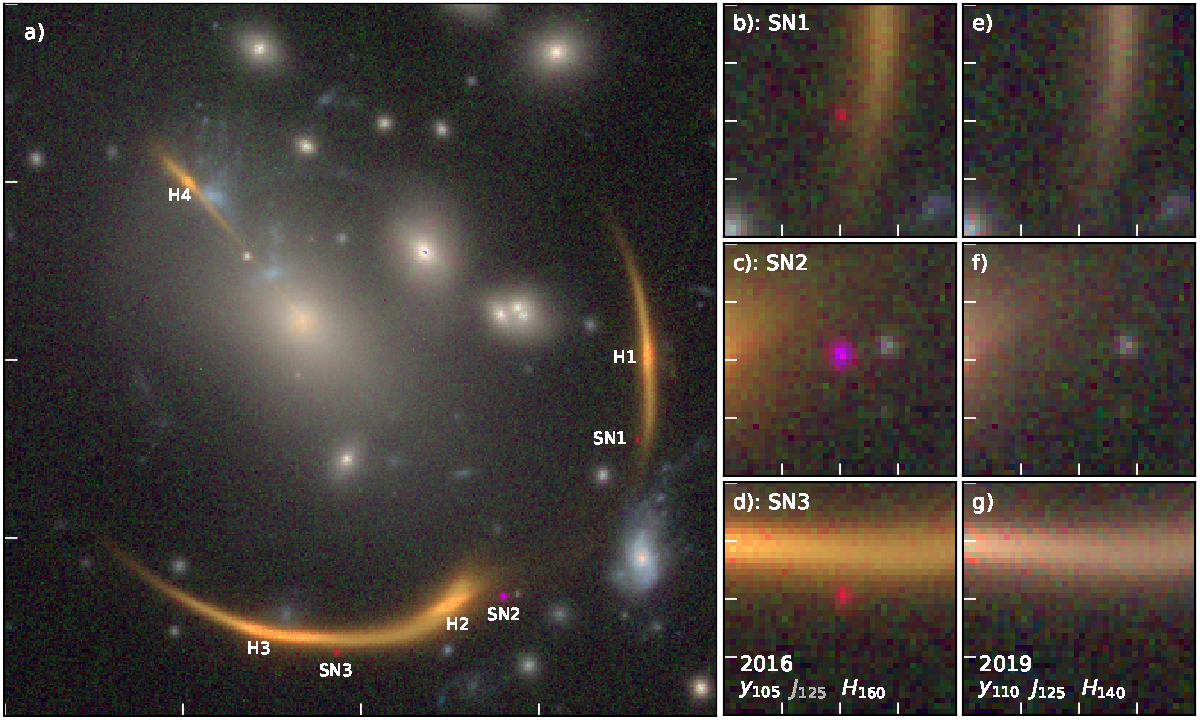
\includegraphics[draft=False,width=0.9\textwidth]{Paper/Figures/fig1_layout.pdf}
    \caption{Overview of the MACSJ0138 cluster field and the locations of the \SNABC images  (SN1--3) and its multiply-imaged host galaxy (H1--4). The wide-field view in $a)$ is 40\arcsec\ on a side with ticks indicating 10\arcsec\ intervals.  
    \added[id=r1]{Labels marked 3.1--3.4 indicate the locations of a separate  multiply-imaged [O\textsc{ii}]-emitter at $z=0.77$ used to help constrain the lensing potential.} 
    Panels \emph{b}--\emph{i} show 4\arcsec\ cutouts around the lensed SN images with 1\arcsec\ ticks.  The three-color images are generated from the WFC3/IR filters as indicated; panels \emph{bcde} show the imaging from 2016 July where the SN was visible and \emph{fghi} show the later imaging from 2019 July where the the SN has faded away.  Panels \emph{aei} indicate the location of the fourth image predicted to appear in $\approx$2037 \added[id=r3]{and panel \emph{a} shows the final and highly demagnified fifth image (``SN5'')}. All panels use the late-epoch F125W imaging for the green channel; nevertheless, it is immediately clear that the SN2 image is substantially bluer than the other two, which helps to constrain the relative age of each SN image and the transient classification as a likely Type Ia supernova explosion. }
    \label{fig:layout}
\end{figure*}


\clearpage
\begin{figure}
  \centering
    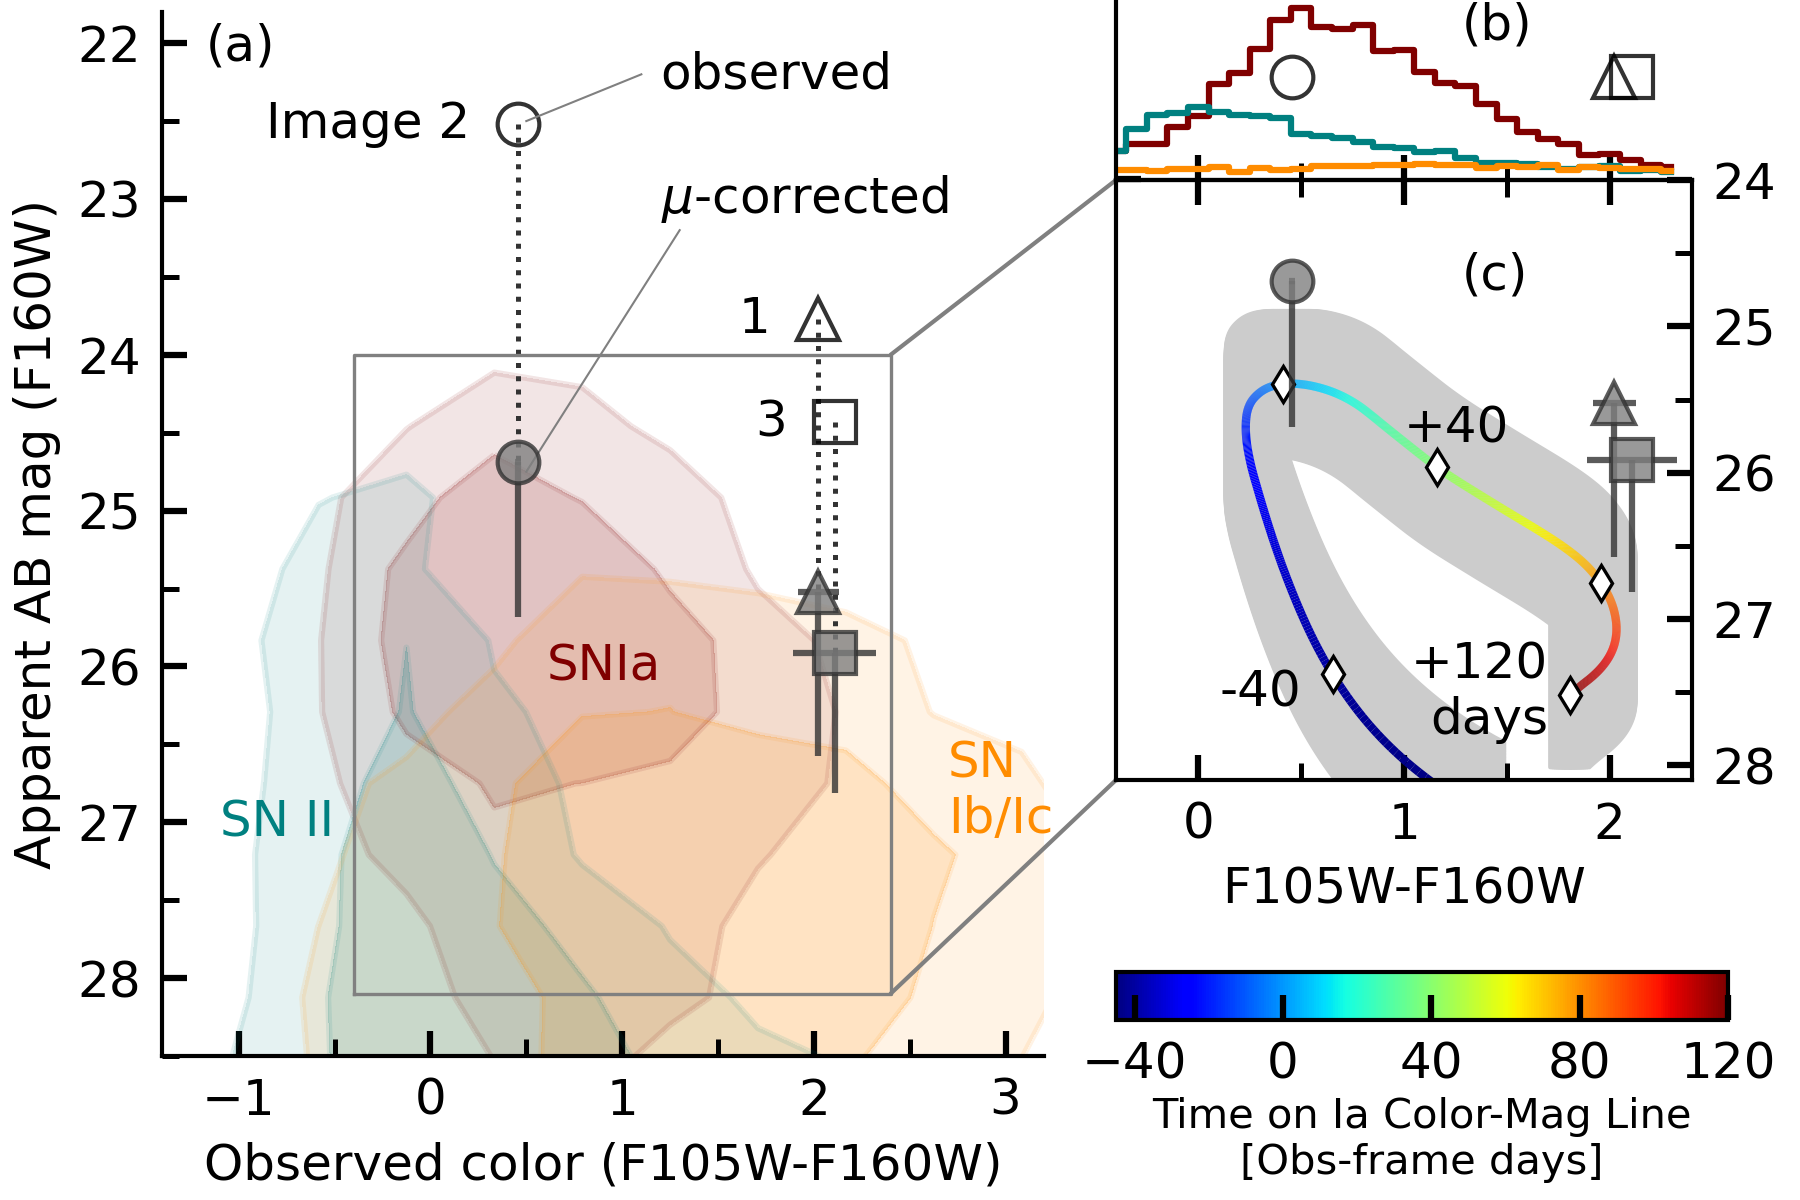
\includegraphics[draft=False, width=\textwidth]{Paper/Figures/snRequiem_classcontours_timeline_hist.png}
    \caption{Classification information for \SNABC based on its position in color-magnitude space. \replaced[id=r3]{(a)}{\emph{Left:}} 
    \added[id=r1]{The observed photometry for the three SN images is shown as open markers. Vertical dotted lines show the lens magnification corrections using our preferred lens model, with a filled grey marker indicating the corrected (demagnified) magnitude. Error bars indicate the observational and systematic uncertainty, including the range of alternative magnification corrections encompassed by lens model variations.} 
    Contours show the population distributions for normal SNe of Type Ia (red), Type Ib/Ic (gold), and Type II (green), drawn \replaced[id=r3]{with two contour levels enclosing }{to enclose} 68\% \deleted[id=r3]{(interior solid lines)} and 95\% \deleted[id=r3]{(exterior shaded regions)} of each SN population.  Each SN sub-class was simulated at $z=1.95$, and samples from their expected light curves were drawn uniformly in time.  
    \replaced[id=r3]{(b)}{\emph{Right:}} \added[id=r3]{Marginalized distributions along the color dimension for the three SN sub-classes (using the same color scheme).  The simulated populations have been scaled according to the expected explosion rates in the SN host galaxy, based on its stellar population properties. Open markers show the observed colors again.}
    \added[id=r3]{(c) Zoomed-in view of the color-mag space marked by the grey box in panel a.}
    The evolution of a typical Type Ia SN at $z=1.95$ \deleted[id=r3]{in observed color-brightness space} is shown by a colored line, with the line color indicating SN age in observer-frame days relative to peak brightness.  White diamonds correspond to the times labeled on the colorbar \replaced[id=r3]{below}{at right}. Grey shading shows the typical range of luminosities \added[id=r3]{and colors} observed for the Type Ia SN population in the nearby universe. %\cite{wang_determination_2006}.
    \added[id=r2]{Although the magnification-corrected data are brighter than expected for most SNIa, they are consistent both with the overall SNIa population, and with the SNIa color-mag vs time curve. } 
    %An interactive 3-D version of this figure is available online at \href{https://plot.ly/~jpierel/6}{https://plot.ly/~jpierel/6}
    \label{fig:class}
    }
\end{figure}


\clearpage
\begin{figure}
    \centering
    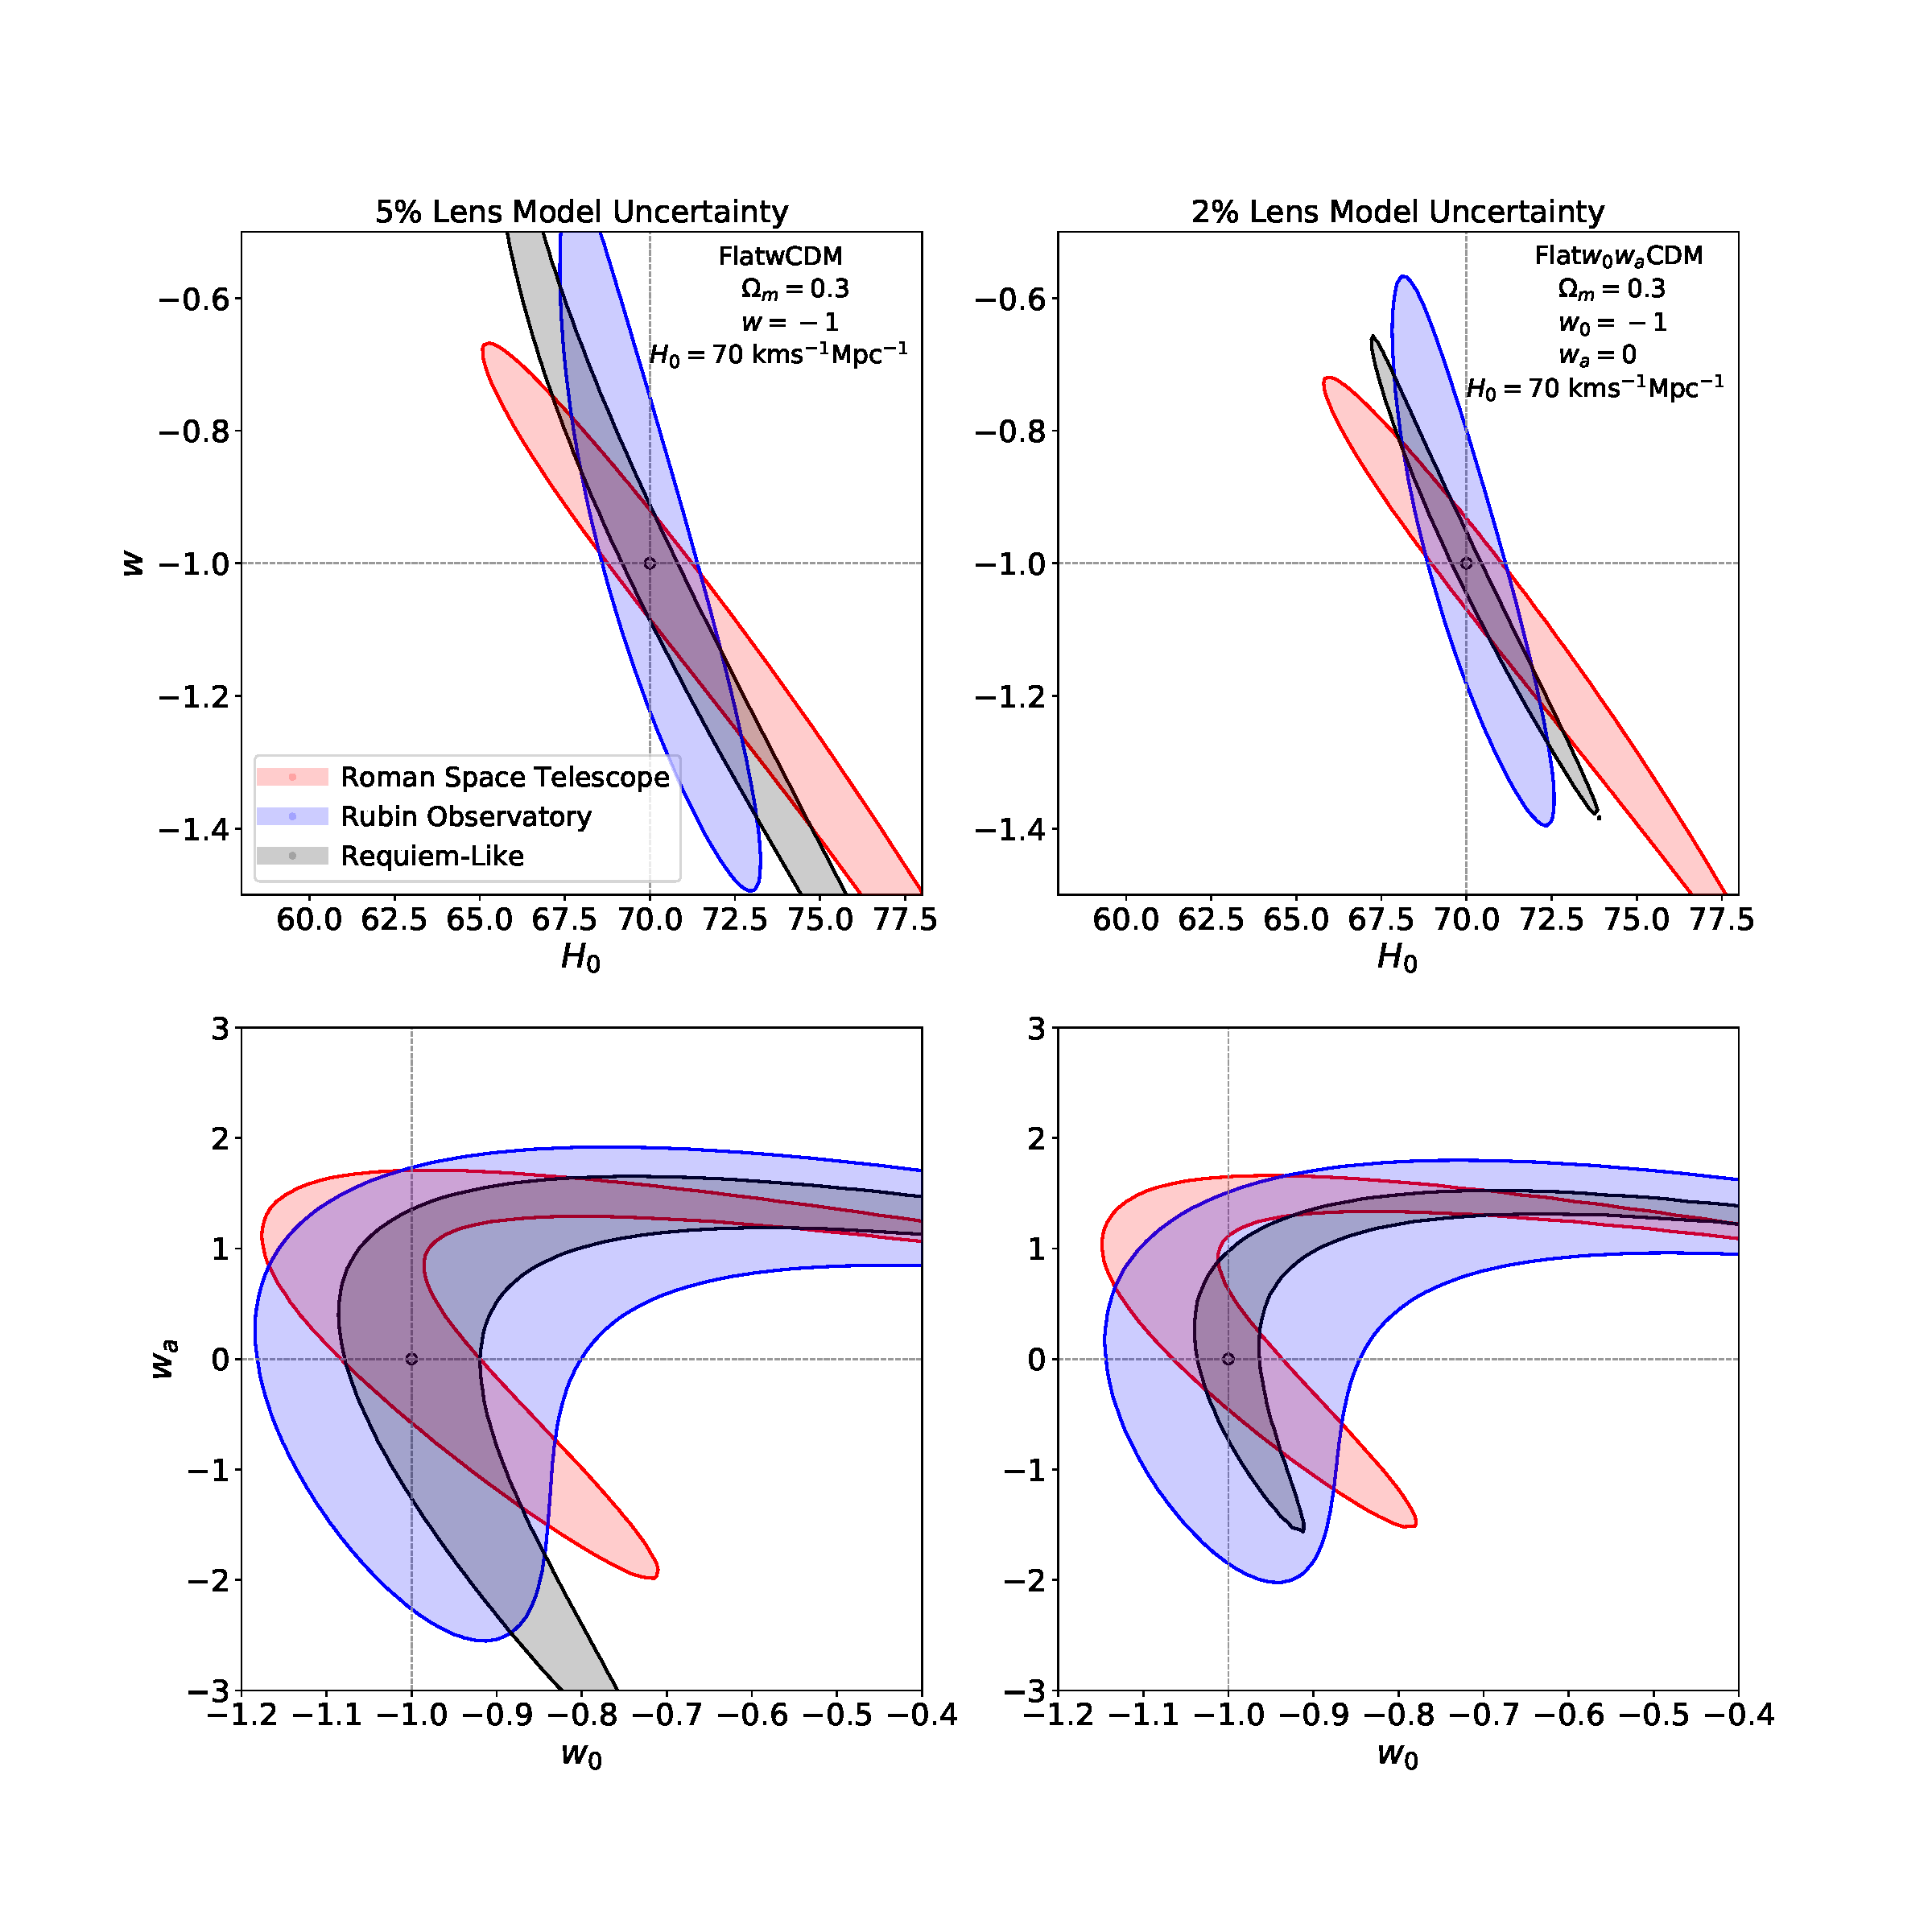
\includegraphics[draft=False,trim={2cm, 3cm, 3cm, 4cm},clip,width=\textwidth]{Paper/Figures/snrequiem_hw_w0wa_apples_to_lsst_ngrst_4panel.pdf}
    \caption{  
    The sensitivity of \SNABC to the expansion rate of the universe ($H_0$) and dark energy equation-of-state parameters ($w_0, w_a$). Dashed lines and the \replaced[id=r3]{black}{white} marker show the input values (upper right of the top panels) that were used for this simulation. Contours show the 1$\sigma$ confidence region for a projected sample of 5 lensed SNIa time delays from the Rubin Observatory (blue) and the Roman Space Telescope (red) compared to 5 events like \SNABC (black).  The left and right columns assume a 5\% and 2\% contribution to the distance uncertainty from modeling the lens potential, respectively. 
    In order to isolate the plotted parameters, all contours are constructed assuming perfect knowledge of the cosmological parameters that are not shown. 
    }
    \label{fig:cosmo}
\end{figure}


\clearpage

\begin{table}
\centering
\begin{tabular}{crc|cc}
    \multicolumn{1}{c}{}&
    \multicolumn{2}{c}{\textbf{Inferred from Photometry}}&\multicolumn{2}{c}{\textbf{Lens Model Predictions}}\\
    %\multicolumn{1}{c}{}&\multicolumn{1}{c}{}\\
    \multicolumn{1}{c}{\textbf{Image}} &\multicolumn{1}{c}{\textbf{Age}} &\multicolumn{1}{c}{$\mathbf{t_i-t_1}$}&\multicolumn{1}{c}{$\mathbf{\mu}$}
    &\multicolumn{1}{c}{$\mathbf{t_i-t_1}$}\\
    
\midrule
\textit{1}  & $92^{+21}_{-19}$ & -- & $5\pm1$ & --\\
\textit{2} & $-24^{+16}_{-7}$ & $114^{+28}_{-31}$ & $7\pm3$ & $82\pm62$ \\
\textit{3} & $107^{+26}_{-21}$ & $-17^{+19}_{-16}$ &$3.9\pm0.5$  & $-19\pm34$ \\
\textit{4} & -- & -- & $0.4\pm0.2$ & $7742\pm540$\\
\textit{5} & -- & -- & $<0.01$ & $9463\pm770$\\


%%%^^^^^^^UPDATE UNCERTAINTIES BASED ON JR^^^^^^^^%%%%%%

% 2020.06.19  OLD DATA (prior to MODEL H) with time delays referenced to image 2.
%\textit{1}  &$79.10^{+45.56}_{-11.76}$&$91.31^{+62.49}_{-23.36}$ &8.942&103.6\\
%\textit{2} & $-16.67^{+19.14}_{-13.10}$&-- \ \ \ \ \ \ \ \ \  & 18.48&-- \ \ \ \ \\
%\textit{3} &$80.46^{+20.10}_{-9.84}$&$92.60^{+37.28}_{-21.76}$ & 13.257&153.8\\
%\textit{4} &-- \ \ \ \ \ \ \ \ \ &-- \ \ \ \ \ \ \ \ \ &1.137&5980.4\\
\end{tabular}
\caption{\label{tab:time_delays}Time Delays.  The combination of the models for the light curve evolution and the lens time delays implies a date of $2037\pm2$ for the peak brightness of Image 4.}
%\todo[inline]{Note: updated to include image 5}.}
\end{table}

\clearpage



%Here you should list the contents of your Supplementary Materials -- below is an example. 
%You should include a list of Supplementary figures, Tables, and any references that appear only in the SM. 
%Note that the reference numbering continues from the main text to the SM.
% In the example below, Refs. 4-10 were cited only in the SM.     


%\section*{Supplementary materials}
%Materials and Methods\\
%Supplementary Text\\
%Figures S1 to S8\\
%Tables S1 to S7\\
%References \textit{(32-68)}
%\clearpage
%\setcounter{table}{0}
%\renewcommand{\thetable}{S\arabic{table}}

%\setcounter{figure}{0}
%\renewcommand{\thefigure}{S\arabic{figure}}

%\setcounter{page}{1}

%\section*{Supplementary Materials for}
%{\bf \large A Gravitationally Lensed Supernova with an Observable Two-Decade Time Delay}


%\author{
% Steven A. Rodney$^{1\ast}$, 
% Gabriel Brammer$^{2\ast}$,  
% Justin D.\,R.~Pierel$^{1}$, 
% Johan Richard$^{3}$, 
% Sune Toft$^{2}$,  
% Kyle F. O'Connor$^{1}$, 
% Mohammad Akhshik$^{4}$, 
% Katherine E. Whitaker$^{2,4,5}$  \\
%\normalsize{$^{1}$Department of Physics \& Astronomy, University of South Carolina,} \normalsize{ Columbia, SC 29208, USA}\\
%\normalsize{$^{2}$Cosmic Dawn Center, Niels Bohr Institute, University of Copenhagen,} \normalsize{Lyngbyvej 2, Copenhagen \O\ 2100 Denmark}\\
%\normalsize{$^{3}$Univ Lyon, Univ Lyon1, Ens de Lyon, CNRS, Centre de Recherche Astrophysique de Lyon \normalsize{UMR5574, F-69230, Saint-Genis-Laval, France}\\
%\normalsize{$^{4}$Department of Physics, University of Connecticut,} \normalsize{Storrs, CT 06269, USA}\\
%\normalsize{$^{5}$Department of Astronomy, University of Massachusetts,} \normalsize{Amherst, MA 01003, USA}\\
%\normalsize{$^\ast$To whom correspondence should be addressed;}\\ \normalsize{E-mail:  srodney@sc.edu, gabriel.brammer@nbi.ku.dk}
%}

%\subsection*{This PDF file includes:}

%Materials and Methods\\
%Supplementary Text\\
%Figures S1 to S8\\
%Tables S1 to S7\\
%References \textit{(32-68)}

%\clearpage
%\end{document}

\section*{Methods}


\subsection*{Observations} % of the SN and Lensing System}

The observations of MRG0138 used in this work are  summarized in Table \ref{tab:observations}.   We processed all HST observations using the {\tt Drizzlepac} software utilities \cite{gonzaga_drizzlepac_2012}, aligned to a common astrometric reference frame and resampled to a pixel scale of 0.1 arcseconds per pixel.  We then identified isolated and unsaturated stars in each image and used them to create an effective point spread function (ePSF) with $4\times$ oversampling, using the {\tt photutils} package from the {\tt astropy} software suite \cite{the_astropy_collaboration_astropy_2018}.   

To measure the SN photometry we followed two tracks.  As our primary method we performed ePSF fitting directly on the F105W ($Y$ band) and F160W ($H$ band) images where the SN was apparent.  This ePSF fitting allowed for a constant background flux to account for both the sky brightness and the background light of the cluster and host galaxy.  
As a second approach, we created ``pseudo-difference images'' by re-scaling the later F110W and F140W images collected in 2019 (in which the SN is not present).  The transmission functions of the F110W and F140W filters are broader than F105W and F160W, and do not strictly overlap in wavelength.  The optimal scaling factor to produce a clean subtraction therefore depends on the spectral energy distribution of the source.  We set the scaling to 0.62 and 1.17 for F110W-to-F105W and F140W-to-F160W, respectively.  These values produced visually clean subtractions of the SN host galaxy MRG0138---meaning that they minimize the residual flux from MRG0138 left behind in the pseudo-difference images.  We then performed ePSF fitting on the SN in each pseudo-difference image, using the same ePSF model as before.   Both sets of photometry agree to within one standard deviation.  The reported photometry in Table~\ref{tab:photometry} are the measurements from the first method (collected directly from the un-subtracted images).  Also reported in Table~\ref{tab:photometry} are flux densities and uncertainties measured within $D=0.^{\prime\prime}7$ circular apertures at the position of the SN1 image in the 2019 \textit{HST} visits where the SN has faded below the detection threshold.

\begin{table}[ht]
\centering
\begin{tabular}{ccccccr}
    \multicolumn{1}{c}{Telescope} & \multicolumn{1}{c}{Instrument} & \multicolumn{1}{c}{$\lambda_\mathrm{obs}$} & \multicolumn{1}{c}{UT Date} & \multicolumn{1}{c}{MJD} & \multicolumn{1}{c}{SN} & \multicolumn{1}{c}{Exp. Time}\\
 & & & & & & \multicolumn{1}{c}{[s]}\\
\midrule
\textit{Spitzer} & IRAC      & $3.6\,\mu\mathrm{m}$      & 2016-03-15 03:44:04 & 57462.156 &   & 212 \\ % AOR r58785536
\textit{Spitzer} & IRAC      & $4.5\,\mu\mathrm{m}$      & 2016-03-15 03:44:04 & 57462.156 &   & 241 \\
\textit{HST}     & ACS/WFC   & F555W                     & 2016-06-03 21:50:43 & 57542.910 &   & 5214 \\
\textit{HST}     & WFC3/IR   & F160W                     & 2016-07-18 23:14:50 & 57587.969 & + & 1611 \\
\textit{HST}     & WFC3/IR   & F105W                     & 2016-07-19 00:43:47 & 57588.030 & + & 3611 \\ 
\textit{Spitzer} & IRAC      & $3.6\,\mu\mathrm{m}$      & 2016-10-13 14:35:13 & 57674.608 &   & 468 \\ % AOR r58289152
\textit{Spitzer} & IRAC      & $4.5\,\mu\mathrm{m}$      & 2016-10-13 14:35:13 & 57674.608 &   & 581 \\
\midrule
\textit{HST}     & WFC3/IR   & F110w                     & 2019-07-13 20:53:16 & 58677.870 &   & 706 \\ 
\textit{HST}     & WFC3/IR   & F140W                     & 2019-07-14 22:16:01 & 58678.928 &   & 353 \\ 
\textit{HST}     & WFC3/IR   & F125W                     & 2019-07-19 21:27:30 & 58683.894 &   & 706 \\ 
\textit{HST}     & WFC3/UVIS & F814W                     & 2019-07-21 18:50:53 & 58685.785 &   & 912 \\ 
\textit{HST}     & WFC3/UVIS & F390W                     & 2019-07-21 19:01:06 & 58685.792 &   & 1272 \\ 
\textit{HST}     & WFC3/IR   & F140W                     & 2019-07-21 22:42:22 & 58685.946 &   & 353 \\ 
\textit{VLT}     & MUSE      & 0.4--0.9$\,\mu\mathrm{m}$ & 2019-09-06 03:56:25 & 58732.164 &   & 2649  \\
\end{tabular}
\caption{Record of MACSJ0138 observations used in this work.  
The two observations from which three images of the SN were detected are marked with a '+' in column six.
\label{tab:observations}
}
\end{table}

\begin{table}[ht]
\centering
\begin{tabular}{cccc}
Image & Obs. Date (MJD) & Filter & Flux density ($\mu$Jy) \\
\midrule
SN1 & 57588.03 & F105W ($Y$) & 0.18  $\pm$ 0.02 \\
SN2 & 57588.03 & F105W ($Y$) & 2.35  $\pm$ 0.02 \\
SN3 & 57588.03 & F105W ($Y$) & 0.09  $\pm$ 0.02 \\
SN1 & 57587.97 & F160W ($H$) & 1.13  $\pm$ 0.04 \\
SN2 & 57587.97 & F160W ($H$) & 3.57  $\pm$ 0.05 \\
SN3 & 57587.97 & F160W ($H$) & 0.61  $\pm$ 0.04 \\
\midrule
SN3 & 58677.87 & F110W ($Y$) & 0.01  $\pm$ 0.02 \\
SN3 & 58678.93 & F140W ($JH$) & 0.02  $\pm$ 0.02 \\
SN3 & 58683.89 & F125W ($J$) & 0.02  $\pm$ 0.03 \\
\end{tabular}
\caption{Photometry of the SN in MRG0138.  The final three rows indicate ``empty'' aperture flux densities measured at the position of SN3 in the 2019 \textit{HST} visits.
\label{tab:photometry}}
\end{table}


\subsubsection*{VLT Spectroscopy}
\label{sec:vltmuse}

We make use of integral field spectroscopic data obtained on the cluster core of MRG0138 with VLT/MUSE, publicly 
available as part of the program 0103.A-0777(A) (PI: Edge). Three exposures of 970\,sec each were taken with a small dithering offset and 90 degree rotations in between. This dataset was reduced and analysed using the MUSE data reduction pipeline v.2.7 \cite{weilbacher_data_2020} for basic calibration (bias, flat-field, wavelength, LSF, geometry) as well as flux calibration, sky subtraction and astrometry.  We  also make use of the self-calibration technique \cite{bacon_muse_2017} to remove illumination systematics, specifically tuned for the case of crowded fields in the central region of galaxy clusters (Richard et al. in prep.). The combined datacube is then processed through {\tt ZAP} \cite{soto_zap_2016} which applies a PCA technique to remove sky subtraction residuals. The final datacube covers the central 1x1 arcmin$^2$ around the cluster center with 0.2\arcsec$\times$0.2\arcsec$\times$1.25\AA\ pixels.

We have extracted spectra for each HST detected source and inspected them for redshift measurements. In addition, we have run the {\tt muselet} software (publicly available as part of the MPDAF package \cite{piqueras_mpdaf_2019}\footnote{\url{https://mpdaf.readthedocs.io/en/latest/muselet.html}}) to search for line emitters not directly associated with HST sources \cite{mahler_strong_2018,lagattuta_probing_2019}. Apart from the lensed quiescent galaxy, we measured spectroscopic redshifts for cluster members and one ring-like background galaxy north of the BCG at $z=0.766$.  \added[id=r1]{Finally, we have measured the velocity dispersion of the BCG to be 390$\pm$10 km s$^{-1}$.  This measurement was not available for use in our blind lens modeling, but could provide a useful constraint for future lens model improvements (Supplemental Note: Future Work).}

\subsection*{Lens Modeling}

In order to correctly estimate the magnification factors, time delays, and predict the appearance of the future images of \SNABC we need to precisely model the mass distribution in the MACSJ0138 cluster core. To do so we make use of the latest version of \lenstool \cite{jullo_bayesian_2007}\footnote{publicly available at \url{ https://git-cral.univ-lyon1.fr/lenstool/lenstool}}, which performs a Bayesian analysis with an MCMC sampler to estimate the best fit and uncertainty on each parameter of the mass distribution. 

The strong-lensing constraints used are the locations of multiple images found in HST and MUSE/VLT. More specifically we group them into 3 systems: (a) the 4 images of the quiescent galaxy hosting MRG0138-SN, (b) the 3 observed images of \SNABC assumed to be at the same redshift, and (c) the diffuse arc-like structure identified in HST and confirmed as an [O\textsc{ii}]$\lambda$3727 emitter in the VLT/MUSE datacube (see previous section). The image coordinates and redshifts used in the lens model are summarised in Table \ref{tab:mulimages}.

\begin{table}[ht]
    \centering
    \begin{tabular}{cccl}
     ID &   R.A. (deg) & Dec. (deg) & $z$ \\
     \midrule
H1 & 24.5099018 & $-$21.9260130 & 1.95 \\
H2 & 24.5132090 & $-$21.9299032 & 1.95 \\
H3 & 24.5164138 & $-$21.9303172 & 1.95 \\
H4 & 24.5176117 & $-$21.9233433 & 1.95 \\
     \midrule
SN1 & 24.5151253 & $-$21.9306659 & 1.95 \\
SN2 & 24.5123198 & $-$21.9297875 & 1.95 \\
SN3 & 24.5100753 & $-$21.9273418 & 1.95 \\
     \midrule
3.1 & 24.5169659 & $-$21.9234814 & 0.7663 \\
3.2 & 24.5151039 & $-$21.9231406 & 0.7663 \\
3.3 & 24.5184361 & $-$21.9264250 & 0.7663 \\
3.4 & 24.5146833 & $-$21.9261020 & 0.7663 \\
    \end{tabular}
    \caption{Multiple images used as constraints in our parametric model. From left to right: image ID, right ascension, declination, spectroscopic redshift.  Coordinates are in the J2000 reference frame.}
    \label{tab:mulimages}
\end{table}

The cluster mass modelling is performed similarly to other massive strong lensing clusters observed with HST \cite{richard_mass_2014}. In summary, the total mass distribution is parametrized as a combination of multiple dPIE (double Pseudo Isothermal Elliptical) profiles describing both cluster-scale and galaxy-scale dark matter haloes. dPIE are elliptical isothermal profiles with both a core and a cut radius where the density flattens and drops respectively. In the case of MRG0138 the mass distribution is dominated by a single mass concentration centered on its Brightest Cluster Galaxy (BCG). We therefore use a single cluster-scale halo at a fixed cut radius of 1\,Mpc.  We add a single galaxy-scale halo on each cluster member, where the shape parameters (halo center, ellipticity) are fixed to their measured HST morphology and their core radius is negligible (fixed at 0.15\,kpc). 
\added[id=r3]{Figure~\ref{fig:model_components} shows the locations of all components of the cluster model, including 32 cluster members (yellow ellipses).} Cluster members were identified by the combination of red sequence selection (based on the F814W$-$F160W color) and MUSE spectroscopy.

\begin{figure}
    \centering
    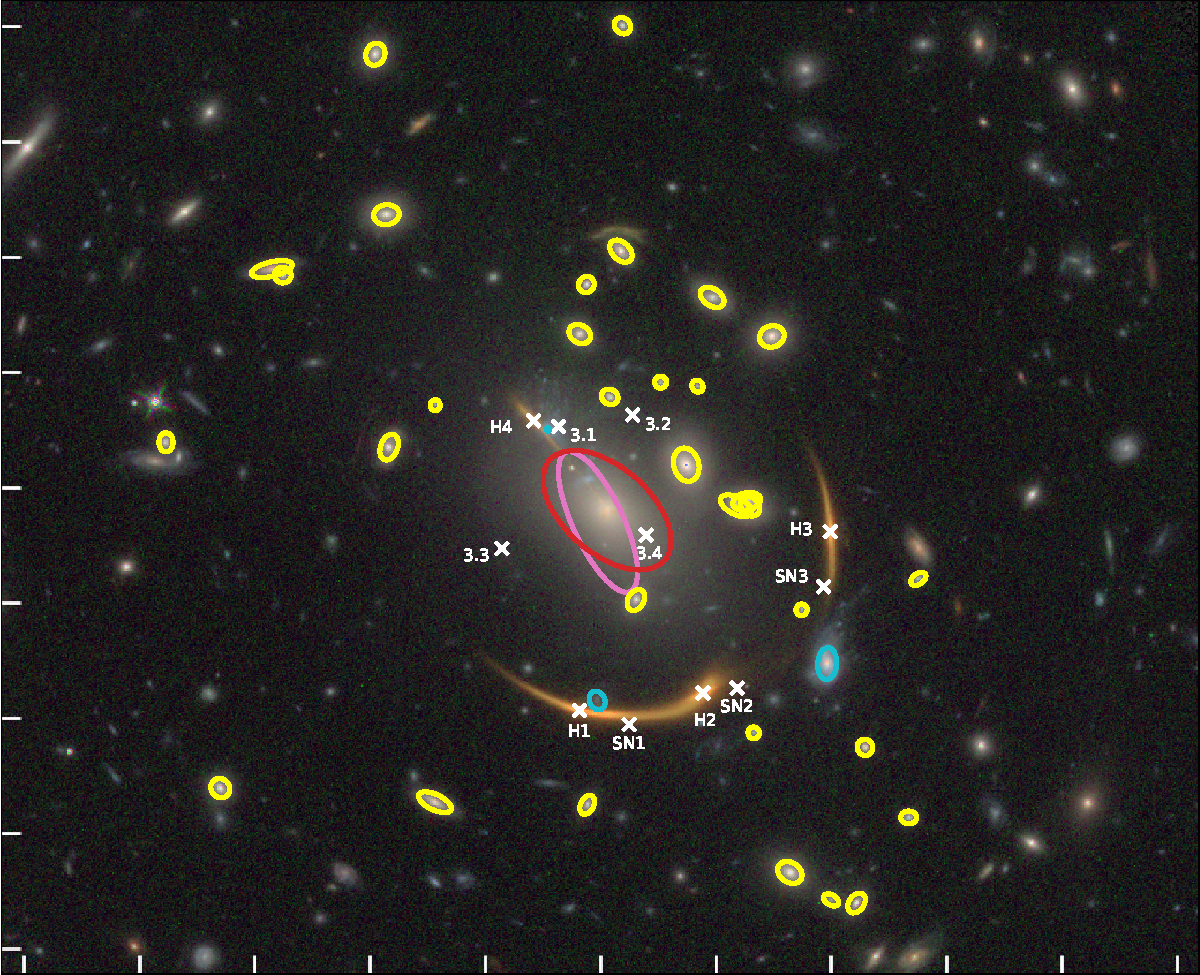
\includegraphics[width=0.8\textwidth]{Paper/Figures/fig4_lensmodel_layout.pdf}
    \caption{\added[id=r3]{
    The elements of the MRG0138 cluster lens model. The model comprises 37 potentials in total: the BCG (red), 32 cluster members (yellow), three perturbers (cyan), and the main cluster potential (pink).  Labeled $\times$ symbols indicate the positions of the SN, host, and one additional multiply-imaged galaxy with a secure redshift used as model constraints (Table~\ref{tab:mulimages}).  The filters used to generate the color image are as in Fig.~\ref{fig:layout}, and tick marks are separated by 10 arcsec.
    } }
    \label{fig:model_components}
\end{figure}


The majority of cluster members are elliptical galaxies selected from the red sequence, and to reduce the number of parameters we assume they follow the scaling relations: $\sigma=\sigma^*\ {\Big(\frac{L}{L^*}\Big)}^{(1/4)}$ for the velocity dispersion, 
and $r_{\rm cut}=r_{\rm cut}^*\ {\Big(\frac{L}{L^*}\Big)}^{(1/2)}$, assuming the Faber-Jackson relation and a constant M/L ratio respectively. $\sigma^*$ and $r^*_{\rm cut}$ are model parameters for a cluster member at the characteristic luminosity $L^*$.  Following the discussion in \cite{richard_locuss_2010} we fix $\sigma^*=158$ km/s and $r_{\rm cut}^*$=45 kpc. 

We individually optimise the $\sigma$ and $r_{\rm cut}$ parameters for 4 specific galaxies which are not expected to follow the aforementioned scaling relations: the BCG and three perturbers P1 to P3. These perturbers are either blue gas-stripped galaxies infalling into the cluster core, and/or located very close to the images of the \SNABC host galaxy, perturbing its apparent morphology with additional lensing. This choice of perturbers is similar to the ones used in the model by \cite{newman_resolving_2018}. 

\lenstool optimises the parameters of the model by minimising the overall root mean square dispersion (RMS) between the predicted and observed locations of the multiple images. The best fit parameters of each mass component are provided in Table~\ref{tab:massmodel}. The error bars are derived from the MCMC models sampling their posterior probability distribution. 

We developed five lens model variants blindly (i.e., without knowing the impact of each lens model variation on the transient classification or time delay inferences). Model A was the first viable model developed, which did not include additional perturbers, and did not include the additional lensed background source at $z=0.7663$.   In Model B we allowed for the location of the main cluster dark matter halo to be free, with an offset from the reference position taken at the BCG center.  Model C allowed the same central position offset and also relaxed the constraints on the BCG ($\sigma$ and $r_{\rm cut}$).  Model D fixed the primary dark matter halo at the BCG center, but still relaxed the constraints on the BCG $\sigma$ and $r_{\rm cut}$.
The final model, and the one selected as the preferred model prior to unblinding, is model E, which includes all four perturbers described above, and includes the additional background object at $z=0.7663$.
\added[id=r3]{Note that all of the lens model variants A-D would give a slightly larger magnification for all  three SN images.  This means that our estimated systematic uncertainties are one-sided, as can be seen on Fig.~\ref{fig:class} and Fig.~\ref{fig:colormag_classification_supplement}.}

\begin{table}[ht]
    \centering
    \begin{tabular}{c|c|c|c|c|c|c|c|}
    Potential & $\Delta$R.A. & $\Delta$Dec. & $e$ & $\theta$ & $r_{\rm core}$ & $r_{\rm cut}$ & $\sigma$ \\
                  & [arcsec] & [arcsec] & & [deg] & [kpc] & [kpc] & [km\ $s^{-1}$] \\
\midrule
Cluster-DM & $ -0.7^{+0.4}_{-0.4}$ & $ -1.2^{+0.4}_{-0.4}$ & $ 0.81^{+0.02}_{-0.13}$ & $114.9^{+2.0}_{-4.1}$ & $31^{+13}_{-12}$ & $[1000]$ & $446^{+52}_{-70}$ \\
BCG            & $[  0.1]$ & $[ -0.1]$ & $[0.52]$ & $[-41.1]$ & $[0.15]$ & $136^{+42}_{-32}$  & $700^{+52}_{-57}$ \\
P1             & $[ 19.2]$ & $[-13.5]$ & $[0.49]$ & $[ 86.2]$ & $[0.15]$ & $[25]$            &  $152^{+30}_{-57}$ \\
P2             & $[ -5.0]$ & $[  6.9]$ & $[0.06]$ & $[  4.4]$ & $[0.15]$ & $[12]$            &  $23^{+111}_{-29}$ \\
P3             & $[ -0.8]$ & $[-16.7]$ & $[0.24]$ & $[-63.1]$ & $[0.15]$ & $[6]$             &  $110^{+35}_{-32}$ \\
L$^{*}$ galaxy &           &           &          &           & $[0.15]$ & $[45]$            & $[158]$\\
    \end{tabular}
    \caption{Best fit model parameters for the mass distribution. From left to right: mass component, position relative to cluster center ($\Delta$R.A. and $\Delta$Dec.), dPIE shape (ellipticity and orientation), velocity dispersion, core and cut radius. The final row  is the generic galaxy mass at the characteristic luminosity L$^*$, which is scaled to match each of cluster member galaxies.  Parameters in square brackets are fixed {\it a priori} in the final model (version E). }
    \label{tab:massmodel}
\end{table}


\begin{table}[tb]
    \centering
    \begin{tabular}{c|l|l|c|c|}
    Image     & R.A. & Dec. & $\mu$ & $\Delta t$ \\
    & & & & [days] \\
\hline 
SN1 & 01:38:03.63     & $-$21:55:50.38         & 5$\pm$1     &  ---\\
SN2 & 01:38:02.96     & $-$21:55:47.26         & 7$\pm$3     & 82$\pm62$ \\
SN3 & 01:38:02.42     & $-$21:55:38.47         & 3.9$\pm$0.5   &   -19$\pm34$ \\
SN4 & 01:38:04.15$\pm$0.36 & $-$21:55:24.73$\pm$0.43 & 0.4$\pm$0.2 & 7742$\pm$540\\
\hline 
\end{tabular}
    \caption{Magnifications and time delays predicted by the lens model at the location of each supernova image. Coordinates are given in the J2000 reference frame, as measured for images 1--3 and as predicted for image 4.  Uncertainties in the predicted position of image 4 are in arcseconds.  Time delays are reported relative to SN1.}
    \label{tab:snpred}
\end{table}

\begin{figure}
    \centering
    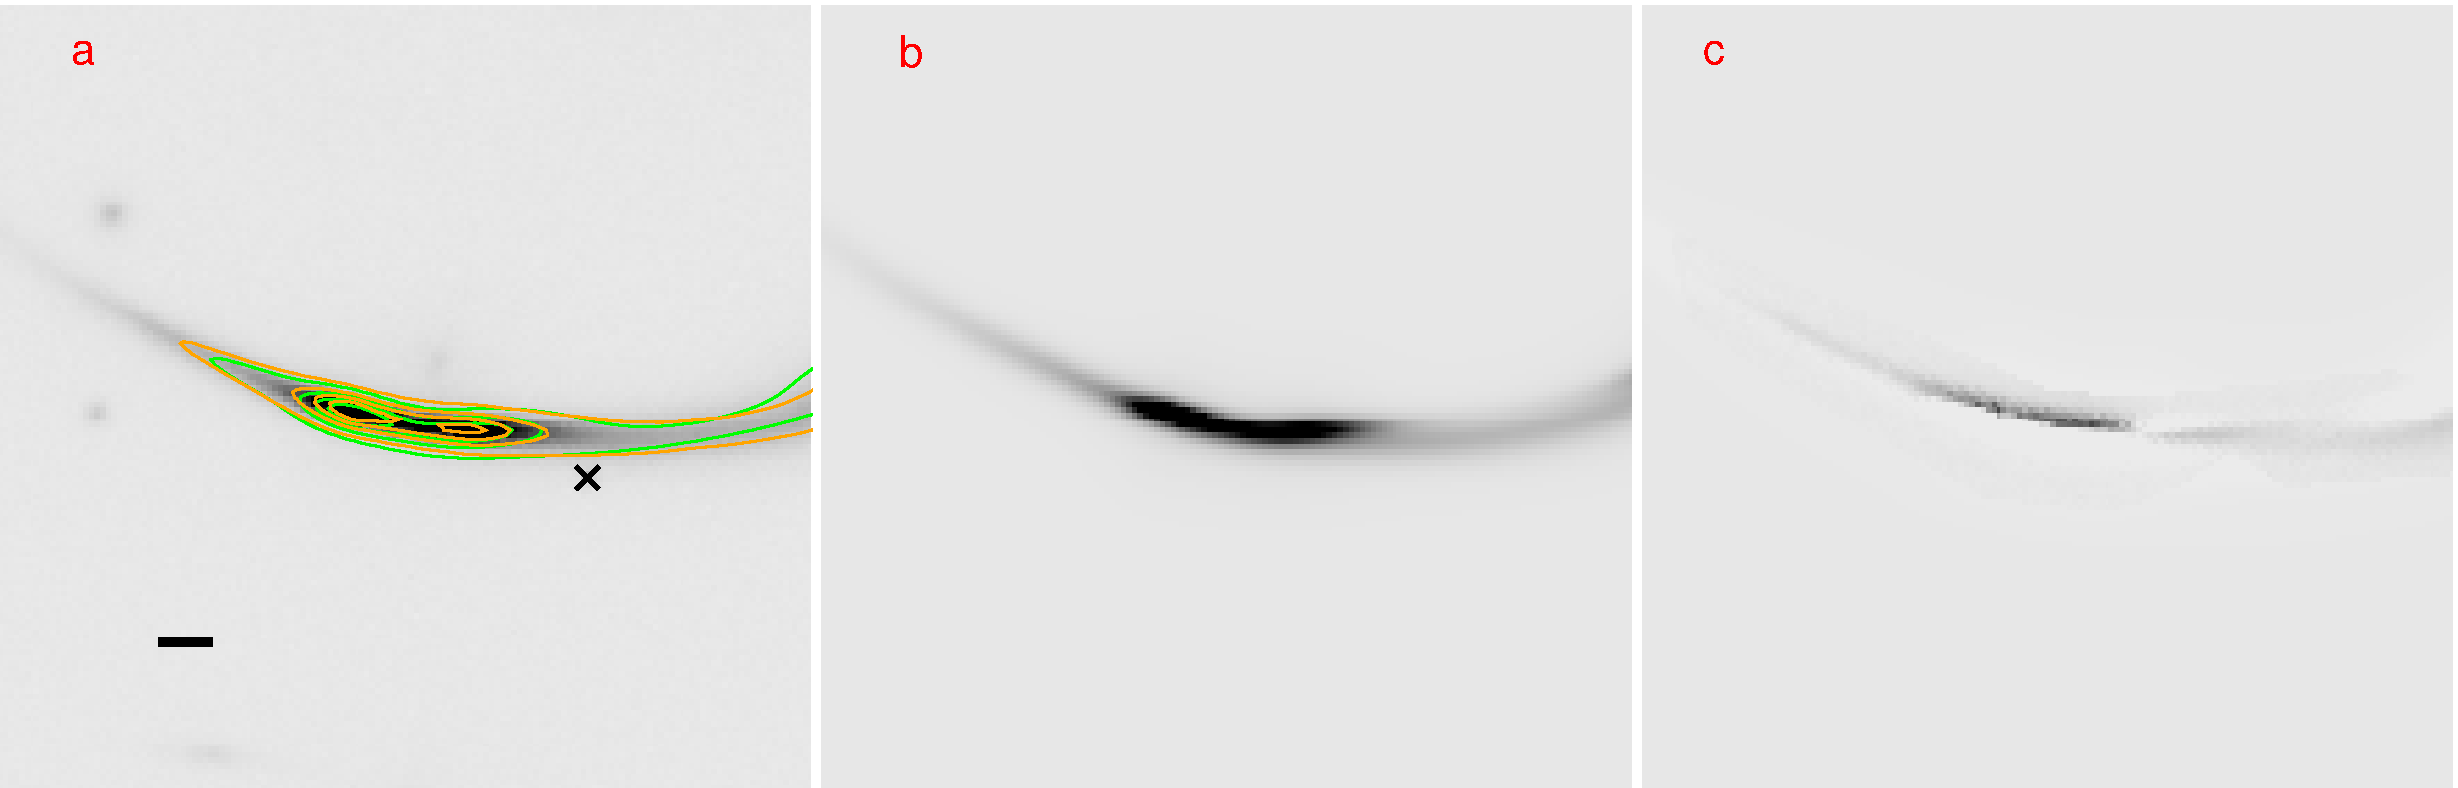
\includegraphics[width=0.75\textwidth]{Paper/Figures/host_image1_resid.pdf}\\
    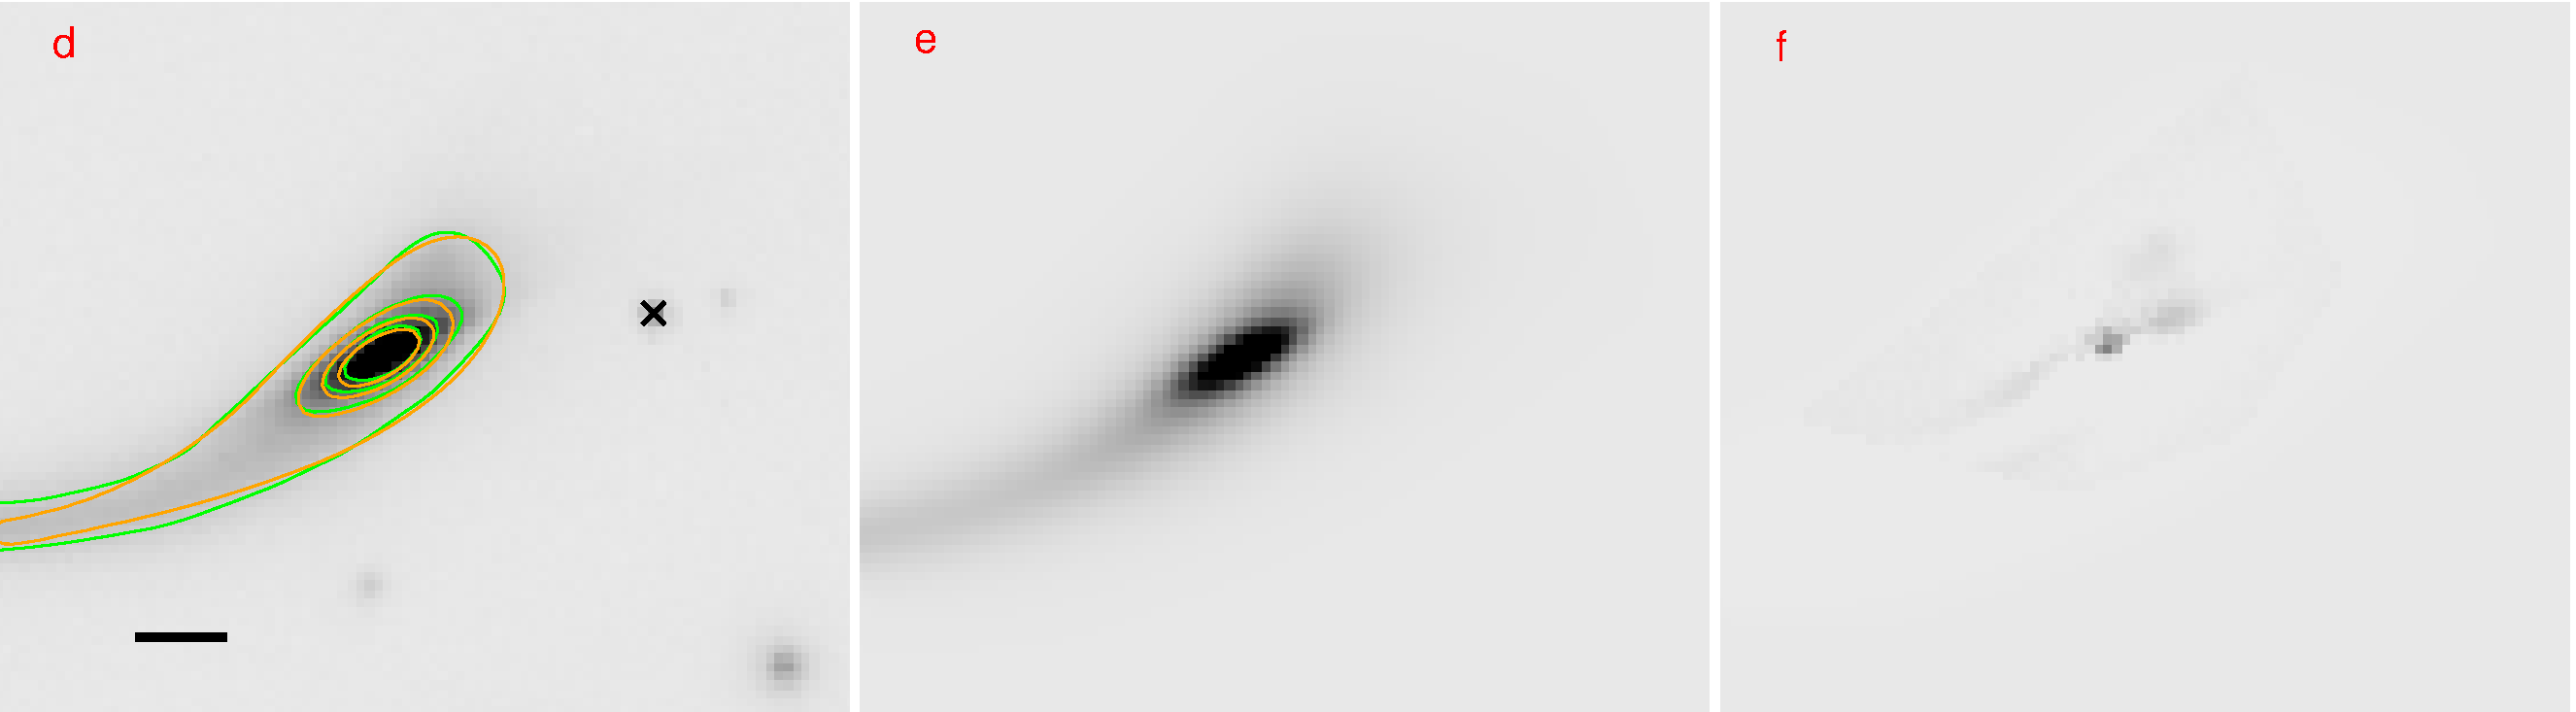
\includegraphics[width=0.75\textwidth]{Paper/Figures/host_image2_resid.pdf}\\
    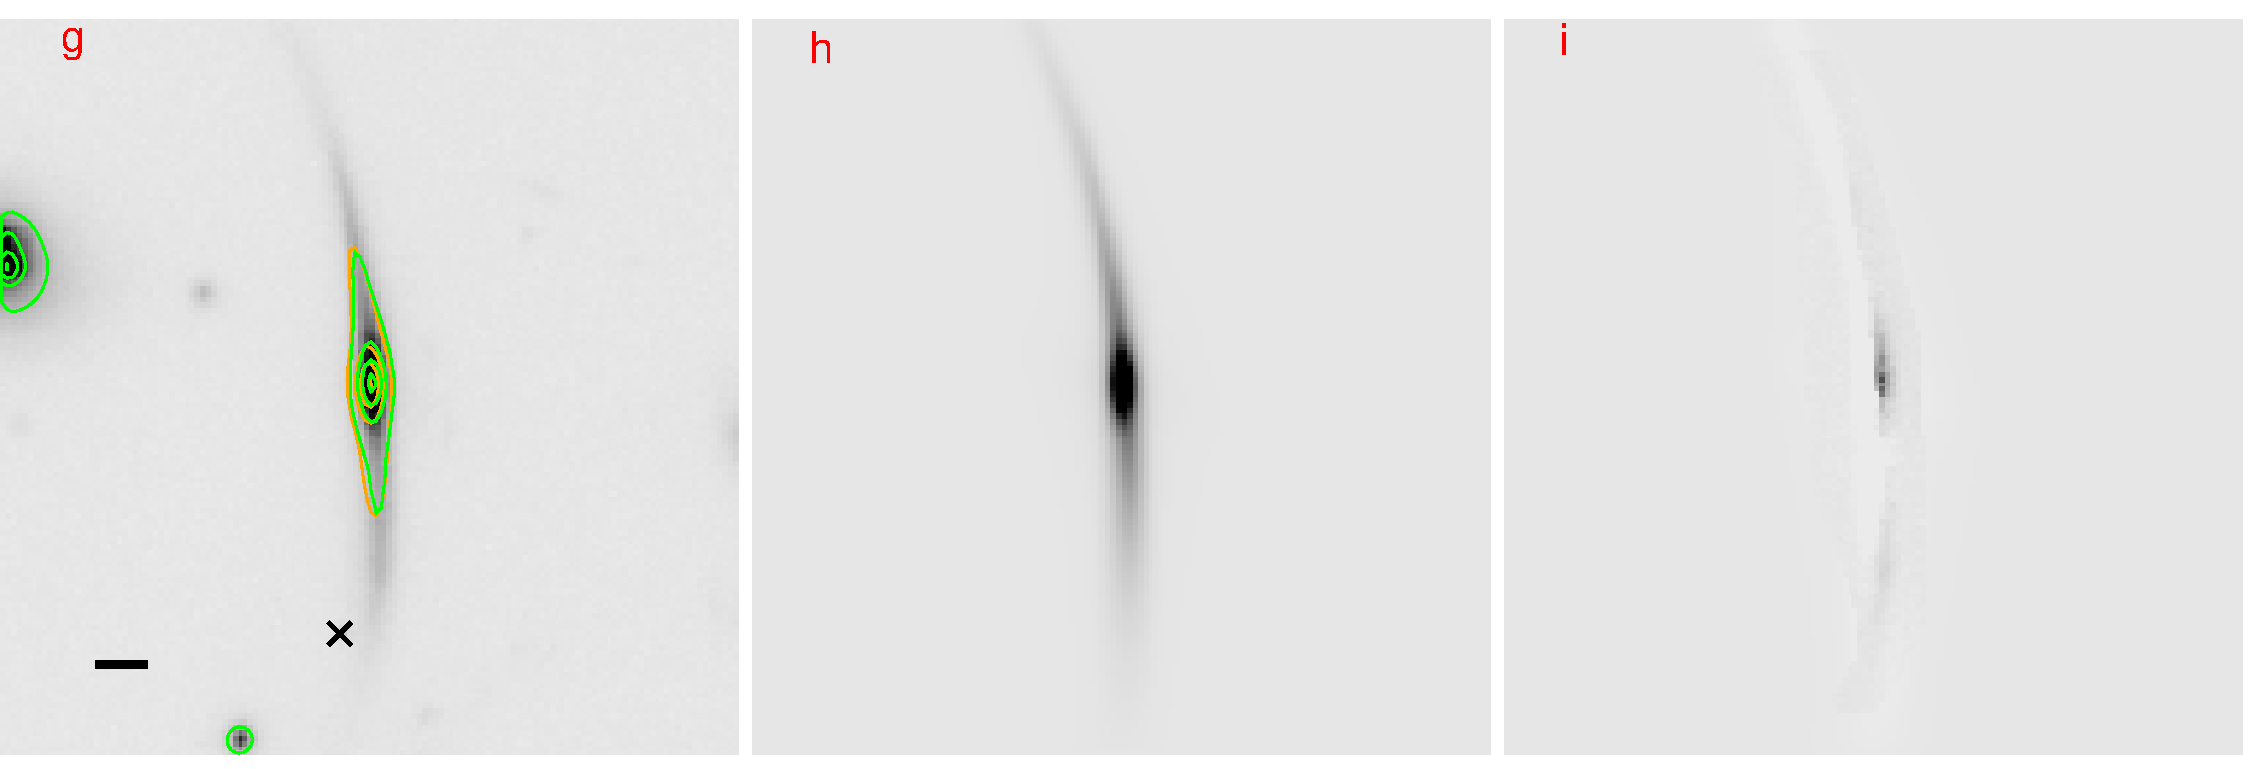
\includegraphics[width=0.75\textwidth]{Paper/Figures/host_image3_resid.pdf}
    \caption{\added[id=r3]{Comparison of the SN host galaxy against a simulation using lens model E. North is up and East is left. Image 1.1 is shown in the top row, 1.2 in the middle, and 1.3 in the bottom. The left column (panels a,d,g) shows each observed image in the F160W bandpass, with a scale bar indicating 1 arcsecond.  The central column (b,e,h) shows a simulated galaxy profile generated using lens model E, with a sum of two Sersic  profiles to represent the background galaxy. The last column (c,f,i) shows the residuals (observed-model). 
    Overlaid contours in the first column show the profile of the observed data (green) and the model (orange).
    Some residual flux is apparent in the difference images, but the overall shape of each image is well matched by the simulated profile and the distortions introduced by lens model E.}
    }
    \label{fig:host_model_residuals}
\end{figure}


The final \lenstool model E reproduces all multiple systems with an RMS of 0.15\arcsec. We also simulated the overall shape of the quiescent galaxy using the sum of two Sersic profiles, and check from the HST residuals that they reproduce the pixel-to-pixel morphology of the arcs\added[id=r3]{, as shown in Figure~\ref{fig:host_model_residuals}}. This model is then used to predict the magnification and time delays for the 3 observed images of \SNABC, as well as the location of the fourth  image, which is still to appear. The actual 1$\sigma$ uncertainty on this location is the ellipse overlayed on top of the bottom cutouts in Fig.~\ref{fig:layout}. As the lens model reproduces the location of the SN images within a small uncertainty, these predictions are computed with \lenstool using the barycenter of all source positions corresponding to images SN.1, SN.2 and SN.3 as the same reference source position. We summarise these predictions in Table \ref{tab:snpred}.
\added[id=r1]{Comparing our lens modeling to the previous  model of this cluster from \cite{newman_resolving_2018}, we find that the magnification estimates are broadly consistent, though systematically lower (Supplementary Note: Comparison to Previous Lens Modeling).}


%\added[id=r1]{

\subsection*{Classification}

The lens modeled time delays between the images are $\sim100$ observer-frame days, 
but we see that three images of the transient are visible simultaneously.
From this we can infer that the visibility time of the transient in the $z=1.95$ rest-frame must be at least $\sim$30 days. 
Similarly, with expected magnifications in the vicinity of $\mu\sim10$, the measured apparent magnitudes near 23 AB mag translate to a rest-frame absolute magnitude near $M_B \sim-19.5$ mag (too bright to be a nova, luminous blue variable, or other low-luminosity stellar transient).
Taken together, these indicators strongly suggest that the transient is a supernova (SN). 

Although we have invoked the lens model in this analysis, we note that the inferences are not strongly dependent on the specific lens model predictions.  To make the observed transient images consistent with a fast or low-luminosity transient, the time delays and/or magnifications would have to be changed by more than a factor of 2.  In the analysis to follow, we will work under the assumption that \SNABC is a SN. 


\subsubsection*{SN Sub-Classification Based on Host Galaxy}
With this transient identified as a SN, we now seek to identify the most likely SN type, under the assumption that it belongs to one of the three most common sub-classes (Ia, II, Ib/c).   We first use two methods that rely only on measured properties of the host galaxy to {\it circumstantially} infer the type. This inference is less strongly dependent on the lens model, helping to reduce any bias associated with a lens model-dependent classification. 

Although Type Ia SNe are found in all types of galaxies, CCSNe are limited to galaxies with relatively young stellar populations.  We can therefore infer some information about the SN type using the observed host properties combined with knowledge of the relative rates of Type Ia and CCSNe in different stellar populations \cite{mannucci_supernova_2005}.  In the case of the host galaxy MRG0138, we have a very well-constrained spectral energy distribution (SED) extending out to far-infrared wavelengths with \textit{Spitzer} IRAC data \cite{newman_resolving_2018,newman_resolving_2018-1}.  
From the SED fitting we derived the host galaxy's 
rest-frame $B-K$ color and absolute magnitude, $M_K$, which serve as proxies for the stellar population age and have been empirically calibrated with SN rates in the local universe \cite{foley_classifying_2013}.  We  adopt a lensing magnification correction using \lenstool model E to get $M_K$. 
The $B-K$ color is not affected by the foreground lens.
Using the {\tt galsnid} method \cite{foley_classifying_2013} we 
derive a $75\%$ probability that \SNABC is of Type Ia (row a of Table \ref{tab:classification}).
\added[id=r1]{
We used host galaxy image 2 for this purpose, with the flux-weighted harmonic mean magnification $\mu=8.3$ to derive $M_K$ (see Table~\ref{tab:mu_comparison}).
We also evaluated the other host galaxy images and found no change in the resulting SN classification probability.}

As an alternative host galaxy classification constraint, we use the derived properties of the host galaxy stellar population directly,  rather than adopting color and magnitude proxies. The MRG-M0138 galaxy has high mass ($\log_{10}(M/M_{\odot})=11.7$) but is a very quiescent galaxy, with a specific star formation rate of $\sim10^{-11.3}$ yr$^{-1}$  and a stellar population that is well-matched by an exponential star formation history with an age of $1.4$ Gyr \cite{newman_resolving_2018}. 
The massive stars that end as CCSN explosions have main-sequence lifetimes of $<40$ Myr \cite{smartt_progenitors_2009},  making it unlikely that CCSN progenitors make up a significant fraction of the MRG-M0138 stellar population---though the high total stellar mass makes it possible that pockets of young stars are present.  We define classification probabilities based on the projected SN rate for each SN sub-class, derived from the host galaxy's stellar mass and star formation rate \cite{li_rates_2012}.  This yields a 62\% probability that \SNABC is of Type Ia (row b of Table~\ref{tab:classification}).

\begin{table}[tb]
    \centering
    \begin{tabular}{lp{1.5in}cc|ccc}
        \multicolumn{1}{c}{Method} & \multicolumn{1}{c}{Data} & Lens info & Priors & p(Ia) & p(II) & p(Ib/c) \\
        \midrule
        a. Host color-mag & Host galaxy rest-frame $M_K$, $B-K$ & $\mu_{\rm host}$ & - & 0.75 & 0.19 & 0.06\\
        b. Host stellar pop. & Host galaxy mass \& star formation rate & $\mu_{\rm host}$ & - & 0.62 & 0.27 & 0.09 \\
        %SN color-mag^{*}$ & SN F105W-F160W color, $m_{\rm F160W}$ & SN magnification & Host: stellar pop. & $0.95\pm0.03$ & $0.01\pm0.01$ & $0.04\pm0.04$\\
        c. SN color-mag & SN F105W-F160W color, $m_{\rm F160W}$ & $\mu_{\rm SN}$ & b & 0.95 & 0.01 & 0.04\\
        d. SN light curve & F105W and F160W SN light curves & $\mu_{\rm SN}$, $\Delta t_{\rm SN}$ & b & 0.94 & 0.06 & $<$0.01 \\
    \end{tabular}
    %\tablenote{*}{Reported uncertainties reflect the range of classification probabilities derived separately from the three SN images.}
    \caption{SN classification probabilities. ``Lens info'' indicates the lensing information used to interpret or derive the 
    observational data: $\mu_{\rm host}$ and $\mu_{\rm SN}$ are the magnifications of the host galaxy MRG0138 and the SN, respectively; $\Delta t_{\rm SN}$ refers to the time delays between SN images 1, 2 and 3. In all cases the preferred \lenstool model E is used.  ``Priors'' indicates the host galaxy classification probabilities that were adopted as priors for the subsequent classification using SN data.}
    \label{tab:classification}
\end{table}

\subsubsection*{SN Sub-Classification Based on SN Photometry}

\begin{figure}
    \centering
    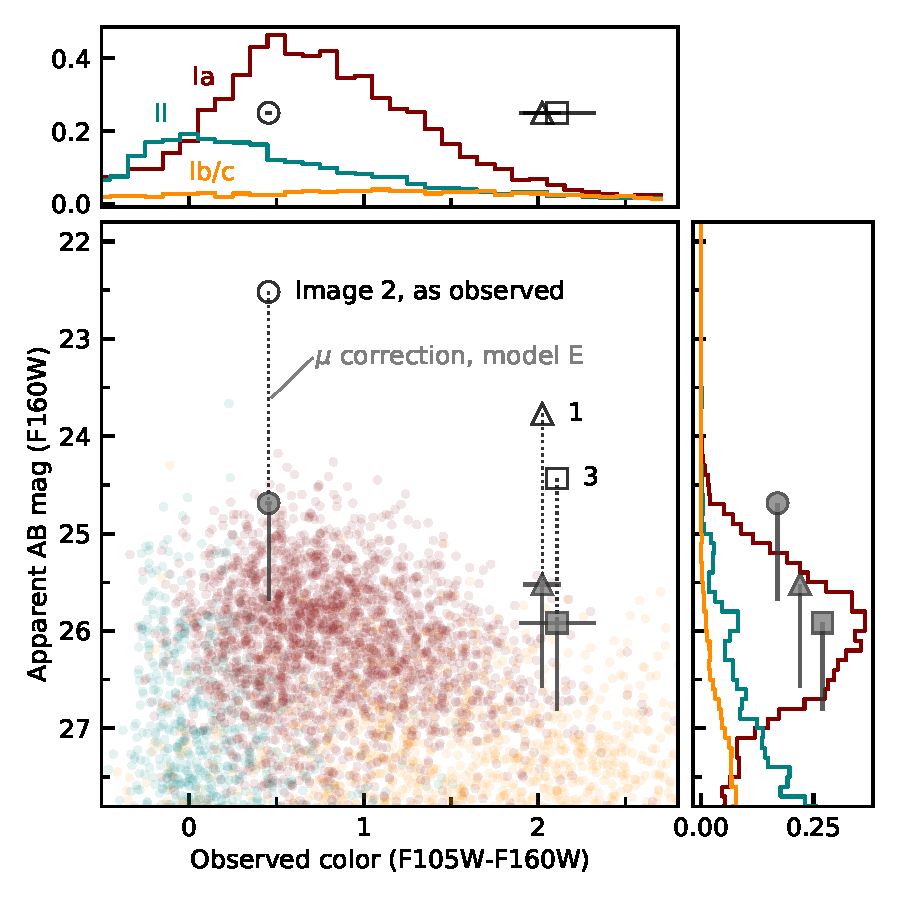
\includegraphics[width=0.9\textwidth]{Paper/Figures/colormag_classification_supplement.pdf}
    \caption{The position of \SNABC in color-magnitude space.
    Colored points show simulated photometry for normal SNe of Type Ia (red), TypeIb/Ic (gold), and Type II (green), with 10,000 simulated SN in each sub-class (not all apparent on this plot).  Histograms above and below show the marginalized distributions that have been rescaled to represent posterior probability density functions. They are normalized to integrate to unity, then multiplied by the SN sub-class priors based on the host galaxy stellar population (row b in Table~\ref{tab:classification}).  Open markers show the observed photometry of the SN. Dotted vertical lines mark the magnification correction based on \lenstool model E.  \added[id=r2]{Closed markers show the resulting magnification-corrected photometry, with asymmetric error bars reflecting the systematic uncertainty derived from the five lens model variants.}  Horizontal error bars in the upper panel indicate the observed uncertainty in 
    the SN color (not affected by lensing).  The relevant SN photometry markers are repeated in the histogram side-panels with arbitrary vertical positions.  All three SN images are located in regions of color-magnitude space that are expected to be dominated by Type Ia SN.}
    \label{fig:colormag_classification_supplement}
\end{figure}

To improve the classification of the \SNABC sub-type, we now bring in observed photometry of the SN itself, and again we adopt two methods.  The first method uses only magnification information from the lens model, and the second uses both the modeled magnification and time delay predictions.  In both cases we adopt the stellar-population-based host galaxy classification probabilities as priors.

Figure~\ref{fig:colormag_classification_supplement} illustrates the first approach.  After applying the magnification corrections, each of the three images of the SN are mapped to color-magnitude space.  We then treat each observed point (each SN image) separately, comparing their color-magnitude location to a simulated population of unlensed SNe.  Our simulation uses the {\tt sncosmo} package \cite{barbary_sncosmo_2016}  to generate 10,000 SN for each of the three principal SN sub-classes (Ia, Ib/c, II), all at z=1.95.  
We then compute the number of simulated SN within a rectangular region around each observed point. The width of this sampling region is set to 3 times the observed color uncertainty, and the height is equal to the lens-modeling magnification uncertainty. \added[id=r2]{The $\mu$ uncertainty used here includes an estimate of the systematic uncertainty for each SN image, derived from the spread of magnifications across lens model variants (similar to the methodology of \cite{newman_resolving_2018}).}  We take the number of simulated SN for each type as an estimate of the likelihood that \SNABC belongs to that class. \added[id=r3]{Note that in this case there is no need to apply a cut to the simulated sample to account for detectability, because the $5\sigma$ limiting magnitude of our HST observations is 26.5 AB mag, and after accounting for magnification of $\sim$1.5 mag (Table~\ref{tab:massmodel}) this becomes $m_{lim}\sim28$ mag. This means that all the points shown in Fig.~\ref{fig:colormag_classification_supplement} (and therefore all simulated SN entering our classification counts) would be easily detectable in our HST imaging.}  Multiplying by the prior probabilities derived from host galaxy properties, we finally derive the probability that the SN is of Type Ia as $p(Ia)=0.92$, 0.98, and 0.95 from the three SN images SN1, SN2 and SN3, respectively. Row c of Table~\ref{tab:classification} reports the mean of our three classification probabilities for each sub-class. 

As a second photometric classification of this SN, we used the {\tt STARDUST2} Bayesian light curve classification tool \cite{rodney_type_2014}, which is also built on the underlying {\tt sncosmo} framework. Here we adopt both the predicted magnifications and time delays from the best lens model, which allows us to put the photometry from the three images together as a composite ``light curve'' and compare against simulated light curves.  {\tt STARDUST2} uses the {\it SALT2-extended} model to represent Type Ia SN \cite{guy_salt2:_2007, pierel_extending_2018} and a collection of 42  spectrophotometric time series templates to represent CCSN (27 Type II and 15 Type Ib/c).  These CCSN templates comprise all of the templates developed for the Supernova Analysis software {\tt SNANA} \cite{kessler_snana:_2009}, derived from the SN samples of the Sloan Digital Sky Survey \cite{frieman_sloan_2008,sako_sloan_2008, dandrea_type_2010}, Supernova Legacy Survey \cite{astier_supernova_2006}, and Carnegie Supernova Project \cite{hamuy_carnegie_2006, stritzinger_he-rich_2009, morrell_carnegie_2012}.  With {\tt STARDUST2} we use a nested sampling algorithm to measure likelihoods over the SN simulation parameter space.  
Figure~\ref{fig:classification_lightcurves} shows the magnification- and time-delay-corrected photometry of \SNABC and \replaced[id=r2]{a random sampling of light curve models from the {\tt sncosmo} nested sampling algorithm employed by {\tt STARDUST2}}{the {\tt STARDUST2} maximum likelihood light curve fits from each of the three SN sub-classes considered (Ia, II, Ib/c).}
\added[id=r2]{Nested sampling is a Monte Carlo method that traverses the likelihood space in a manner that samples the Bayesian likelihood \cite{skilling_nested_2004}.  These sample light curves and color curves therefore give a visual representation of how well each SN sub-class (Ia, II, Ib/c) can match the observed data.}
This figure shows that the limited photometric data can be reasonably well fit by at least one model from any of these three sub-classes. 
\added[id=r2]{The density of curves in the top panels demonstrates that the SNIa model is consistently a good match to the data.} However, the range of model parameters that allow such a fit to the data is much more limited for the heterogeneous CCSN types. \deleted[id=r2]{than for the Type Ia class.}
To compute the posterior probability distribution we adopt priors for each of the three SN classes, again using the classification probabilities derived from the \SNABC host galaxy stellar population properties (row b of Table~\ref{tab:classification}). 
Marginalizing the posterior  probability distributions over all free parameters, we find a 94\% probability that \SNABC is of Type Ia (row d of Table~\ref{tab:classification}).  


%The observed photometry for SN Requiem is consistent with the expected color and magnitude of a Type Ia SN at $z=1.95$, after correcting for lensing magnification using the $\mu$ values from Table~S2.  The magnification-corrected photometry is inconsistent with Type II SNe, which are fainter and more blue. SN Requiem is marginally consistent with the CCSN Type Ib/Ic sub-class, although the image 2 point falls outside of the 95\% confidence region for that population. The three SN Requiem data points are also consistent with the expected time-dependence  of a Type Ia SN in color-magnitude space. Visualizing the changing color and brightness of a SNIa at $z=1.95$ in the F105W and F160W bands, we see that it  would intersect image 2 near peak brightness and approach the image 1 and 3 photometry at roughly 80 observer-frame days after peak (see main text Fig \ref{fig:class}).  


\begin{figure*}
    \centering
%    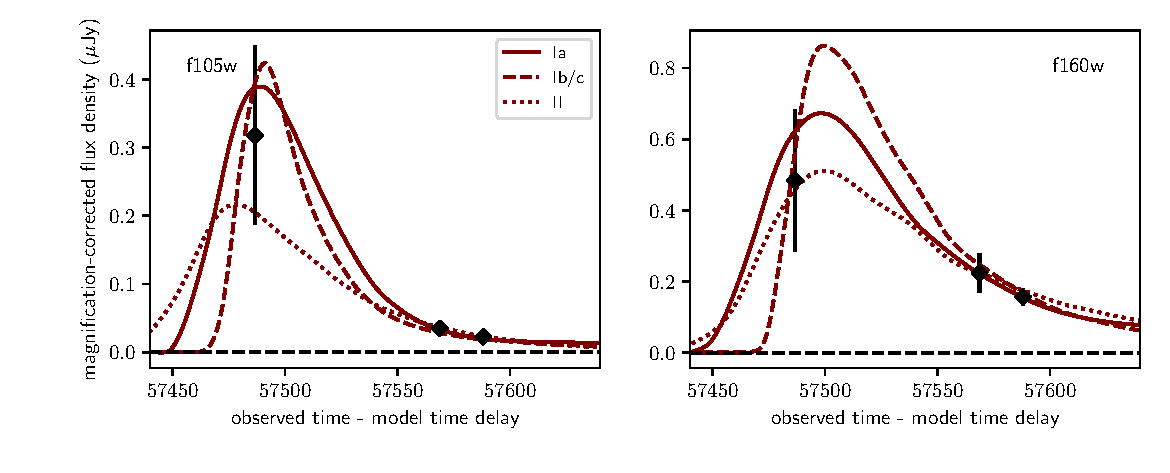
\includegraphics[width=\textwidth]{Paper/Figures/snRequiem_stardust_classify_alltypes.pdf}
\vspace{0pt} 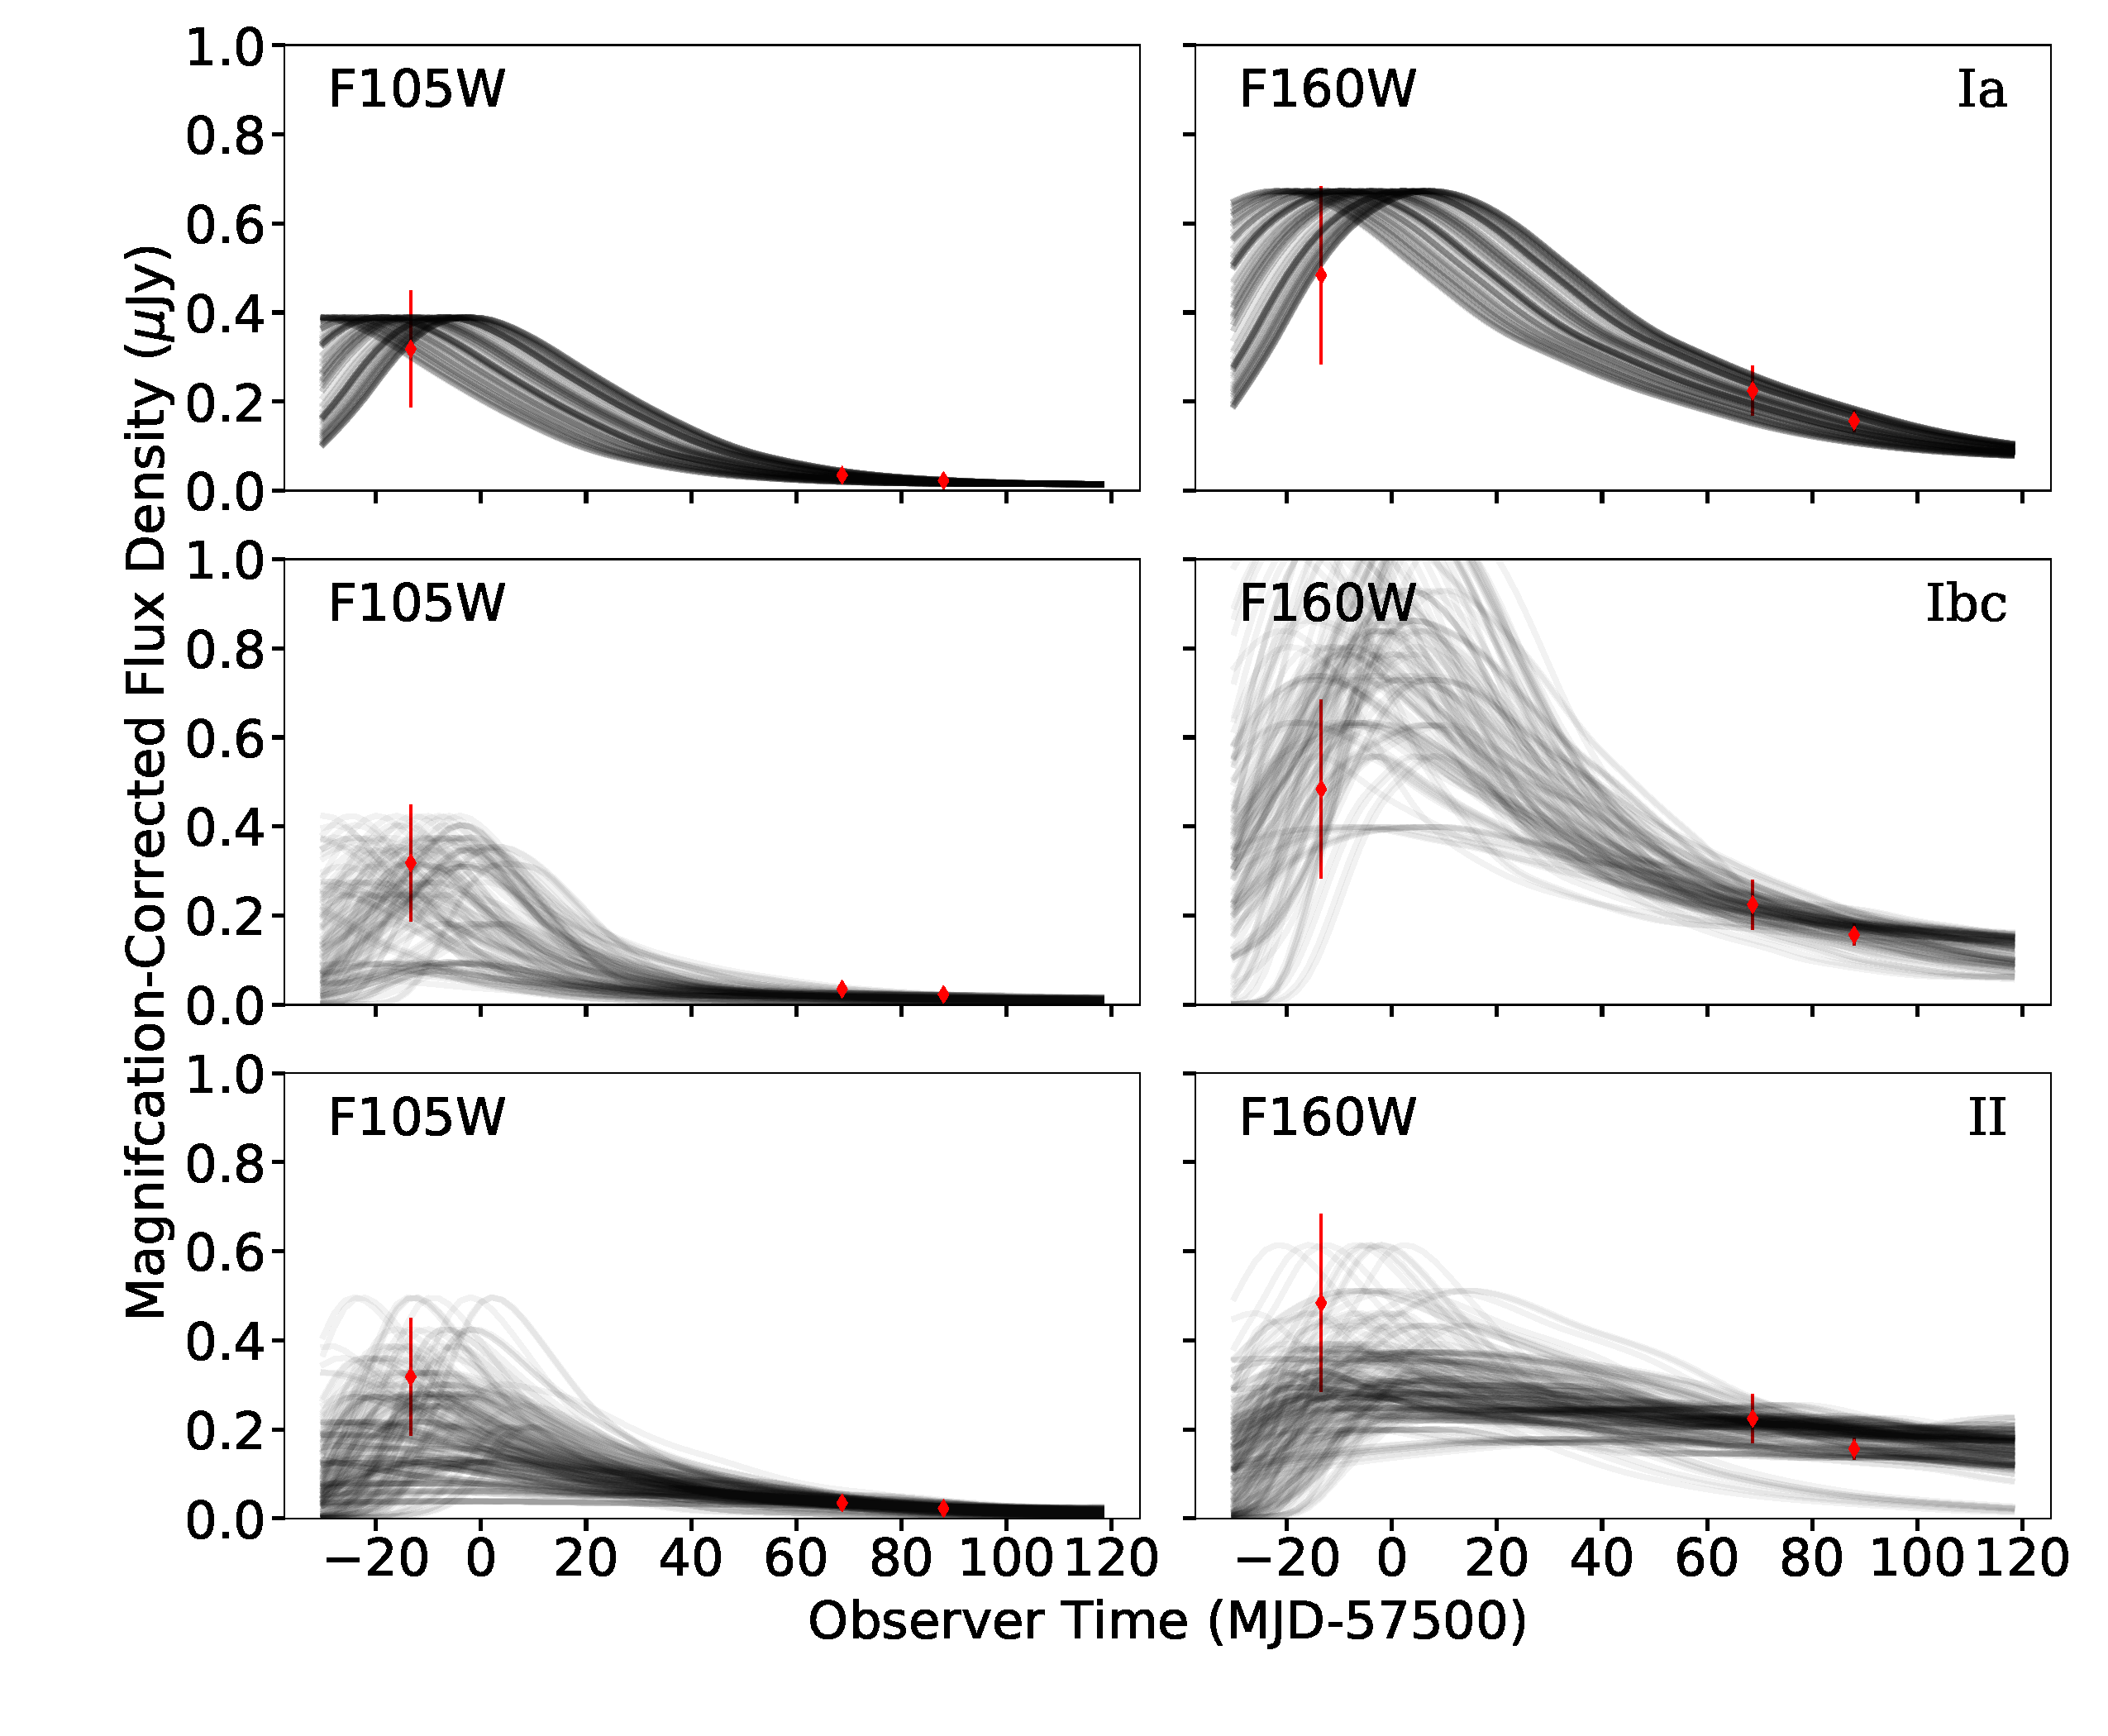
\includegraphics[width=0.63\textwidth]{Paper/Figures/lightcurves_NSAMPLES.pdf} 
\vspace{0pt} 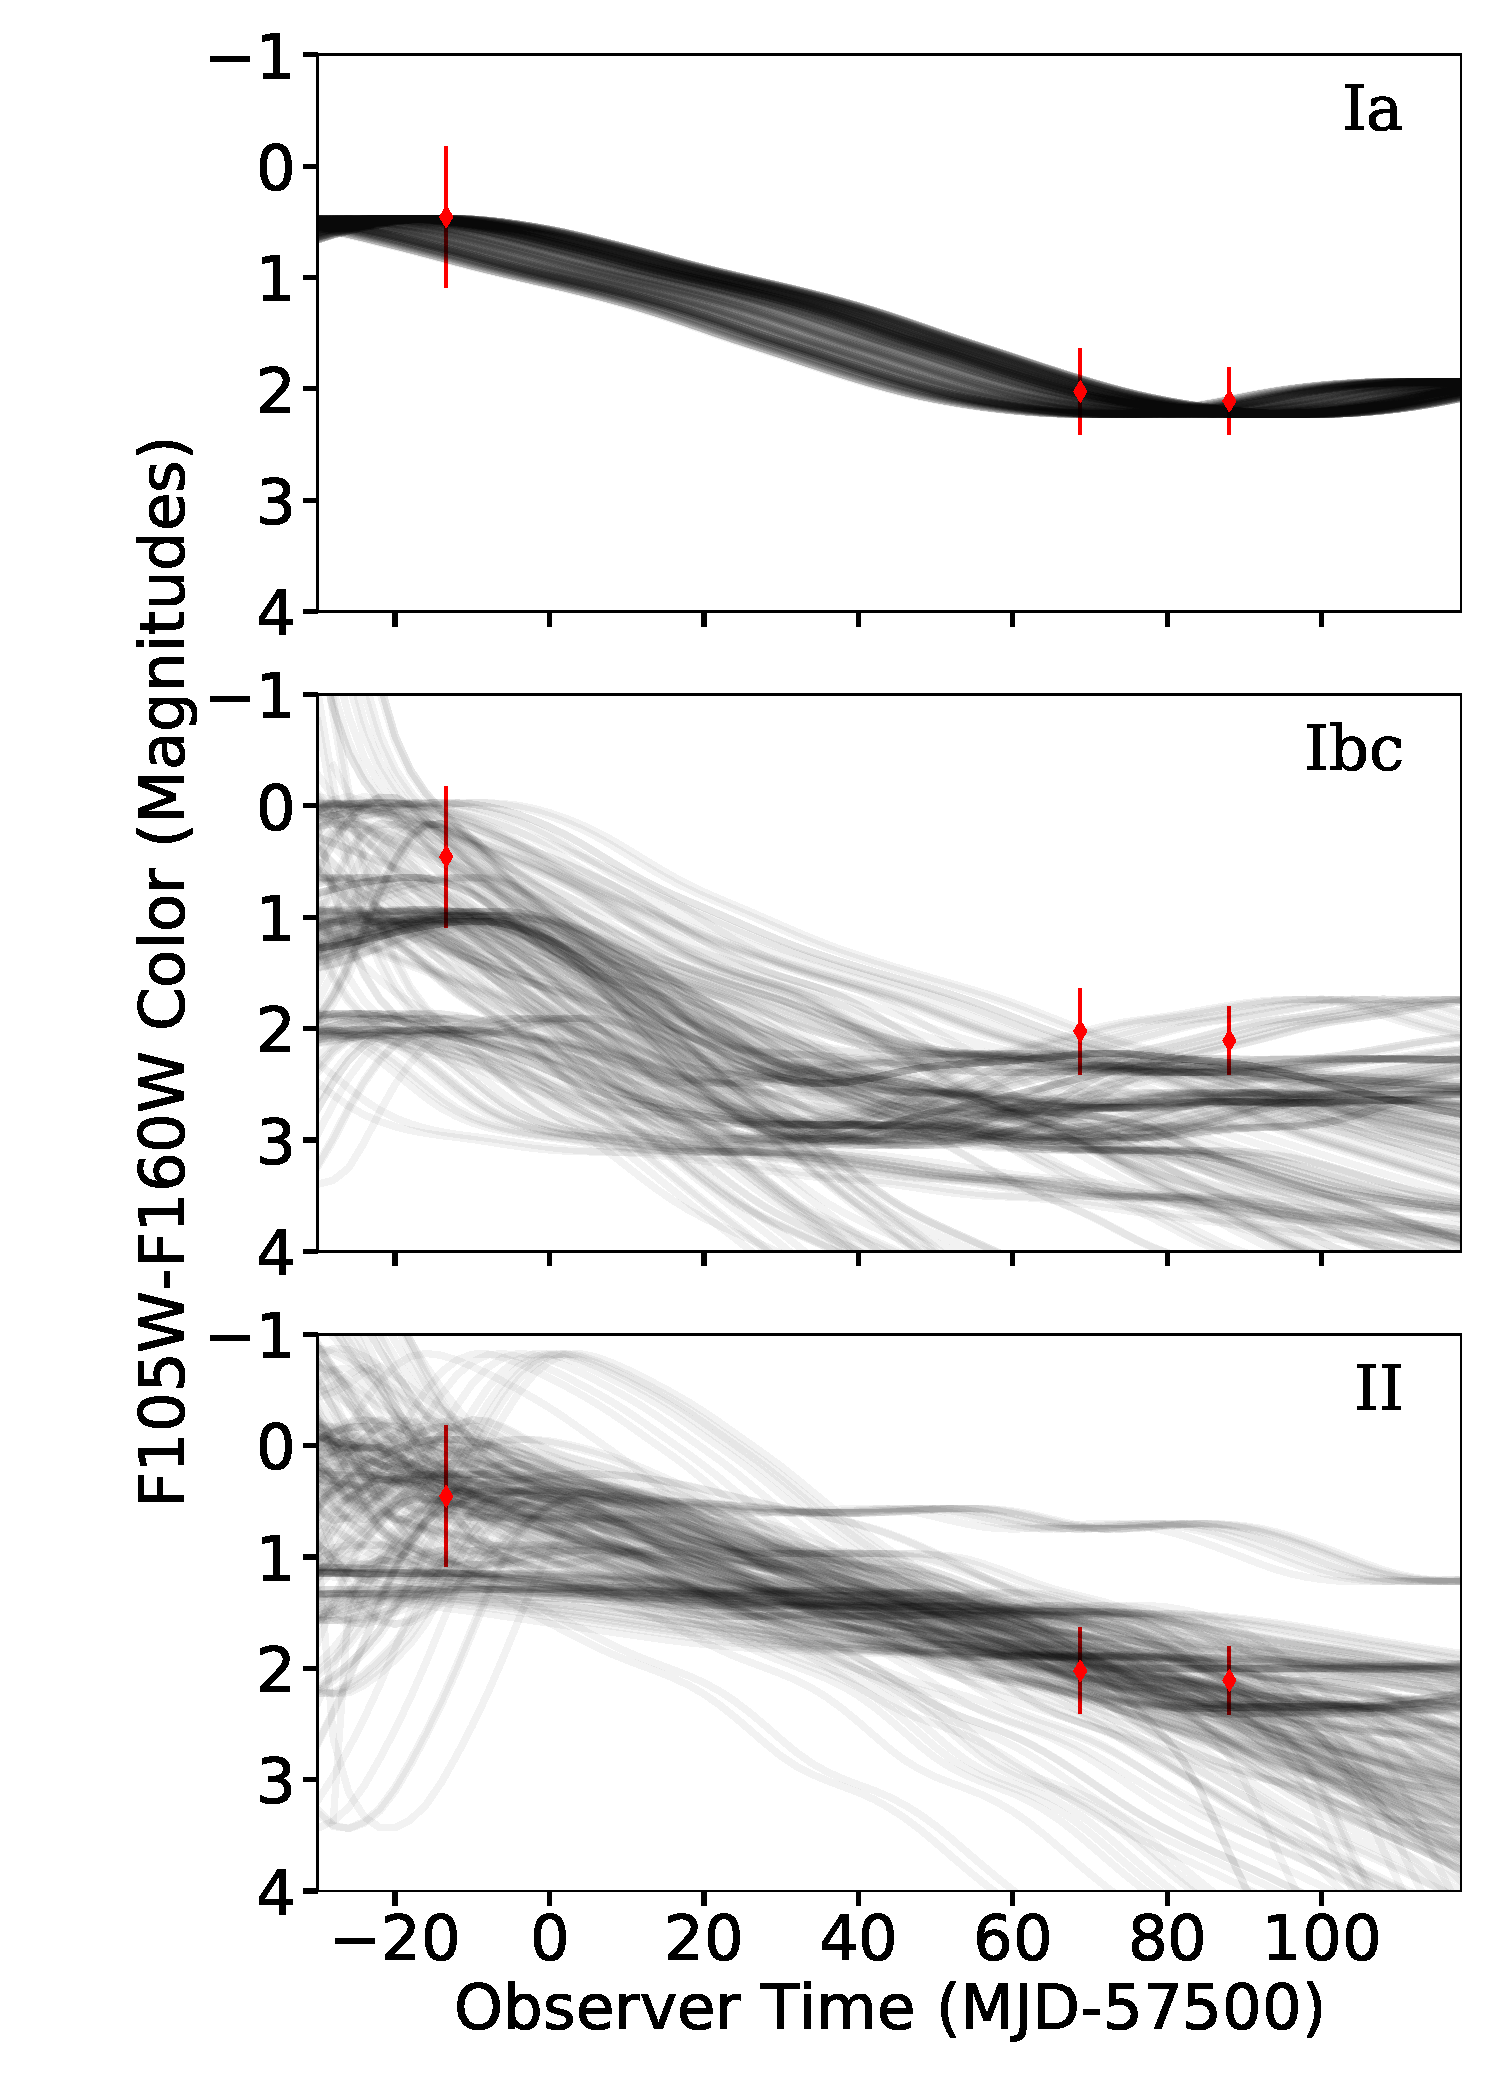
\includegraphics[width=0.36\textwidth]{Paper/Figures/colorcurves_NSAMPLES.pdf}
    \caption{
    \replaced[id=r2]{A representative set of light curve and color curve models from the STARDUST2 classification algorithm.  Panels on the left and center columns show  F105W and F160W, respectively, plotting the model light curves in black and photometry as red markers.  The right-most column shows the F105W-F160W color curves and color data.}{Maximum likelihood light curve fits for each of the three primary SN sub-classes (Type Ia, Ib/c, and II). } All data points 
    as shown have been corrected for magnification and shifted in time using the preferred \lenstool model E. Plotted error bars include the measurement uncertainty and the lens modeling magnification uncertainty. \added[id=r2]{Data points in the right column also include this magnification uncertainty, even though cluster-scale lensing is achromatic, because the {\tt STARDUST2} analysis was done on the light curve data, not the color data directly.} In all panels the first data point is SN image 2, followed by image 1 and image 3. \replaced[id=r2]{In each panel the black curves show 200 SN light curve models drawn at random from the nested sampling sequence of the STARDUST2 (sncosmo) classification. 
    %The distribution of light curve and color curve shapes illustrates the exploration of the multi-dimensional parameter space executed by the nested sampling algorithm as it measures the likelihood for each SN class by comparison with the observed data.
    }{The best-fitting Type Ia, Ib/c and II light curves are shown as solid, dashed, and dotted lines, respectively.}
    \label{fig:classification_lightcurves}
    }
\end{figure*}

The combination of evidence from the derived host galaxy properties  and SN photometry supports the conclusion that \SNABC  is  a Type Ia SN with $>90\%$ confidence.  Although we have adopted some lens modeling corrections for all of these methods, this conclusion is not sensitive to the choices we can reasonably make for modeling the lens.  As shown in Figure~\ref{fig:colormag_classification_supplement}, every  \lenstool model we have evaluated locates the \SNABC  de-magnified position within the region of color-magnitude space dominated by Type Ia SN. Dust is also not a confounding factor here. 
The simulations used in both SN-based classification methods (c and d in Table~\ref{tab:classification}) include dust extinction at the source plane.  If a significant screen of dust exists in the lens plane, this would have the effect of making the SN appear dimmer and more red, so correcting for that extinction would move the \SNABC points upward and leftward on Figure~\ref{fig:colormag_classification_supplement}, which would not shift it into the regions occupied by Type II and Ib/c SN. 


%\subsection*{Measuring the Age of the SN for each Image}
\subsection*{Time Delay Estimation}

We constrain the relative time delays of \SNABC by using two separate methods to estimate the age of the SN at each image during the single observed epoch. The preferred method of SN time delay measurements involves measuring the time of peak brightness for the SN at each image by fitting the light curves, and taking the difference between each measurement as the relative time delay \cite{pierel_turning_2019,dhawan_magnification_2019,huber_strongly_2019}. With only a single observed epoch, this method is impossible due to model parameter degeneracies, and we must rely on color and brightness to constrain the age of each image of the SN. Such age estimates are sometimes referenced to the time of explosion, but in this case we use the observer's convention, setting age=0 as the time of peak brightness in the rest-frame B band ($\lambda\sim4500$ \AA).  Each of these images stems from the same SN explosion, so the difference between the measured age of each image is also a measure of the relative time delay. 

\added[id=r2]{
In all of the light curve fitting exercises described below, we also fix the SALT2 ``stretch'' parameter at $x_1=0$. This parameter defines the shape of the SN Ia light curve (the rate of decline in brightness). If we  allow $x_1$ to be a free parameter, there is no useful constraint on it.  It is highly degenerate with the time delay between the images, which is of course a free parameter in all the fits.  
As a check, we have also tried fixing $x_1$ to other values from $-1$ to $+1$, and the time delay results change by less than 5 days, which is well within all error bars.   
Fixing $x_1$ in this way is comparable to the analysis that will be possible in the 2030s when the fourth SN image is observed. We expect that a SALT2 fit to a well-sampled light curve from the fourth image will provide a tight constraint on $x_1$.  That measured $x_1$ will then be propagated back as a fixed parameter (with small uncertainty) into revised fitting of the SN images 1-3. }

\subsubsection*{Color Curve Age Constraints}

We first attempt to constrain the relative time delays using the color of each observed image, which is independent of the lens model and possible because the phenomenon of gravitational lensing is intrinsically achromatic. One important caveat to this principle is that {\it microlensing} effects are not generally achromatic, because the microlensing caustics may cause differential magnification on the scale of the SN radius \cite{goldstein_precise_2018,foxley-marrable_impact_2018,bonvin_impact_2019}.  Hence, if the expanding SN shell has a color gradient then microlensing may introduce spurious features in the observed colors of the SN \cite{kochanek_quantitative_2004,vernardos_joint_2018}.   Goldstein et al. \cite{goldstein_precise_2018} found that such chromatic microlensing is most likely not present for lensed Type Ia SNe in the period up to about 25 rest-frame days after explosion ($\sim$15 observer days after peak brightness for \SNABC). Only image 2 is likely in the achromatic microlensing phase, but Goldstein et al. \cite{goldstein_precise_2018} found extremely small deviations in the rest-frame $U-V$ color curve due to microlensing at the 68\% confidence interval, and up to a $\sim0.2-0.4$ mag difference with 99\% confidence. While such extreme microlensing could alter the results for images 1 and 3, it would not alter the measurement of image 2 as it is likely in the achromatic phase.
\added[id=r1]{Fortuitously, images 1 and 3 are minima, which are less susceptible to high deviations owing to microlensing when compared to image 2, which is a saddle.}

We use version 2 of the SuperNova Time Delays (SNTD) package\footnote{The v2.0 release is at \href{https://github.com/jpierel14/sntd/releases/tag/2.0}{github.com/jpierel14/sntd/releases/tag/2.0} with documentation at 
\href{https://sntd.readthedocs.io/en/latest/}{sntd.readthedocs.io}}, which has several improvements over the original SNTD package \cite{pierel_turning_2019}. The SNTD package employs a nested sampling algorithm within three separate methods to measure time delays, and is designed to fully utilize the information present in SN light curve templates \cite{hsiao_k_2007,guy_salt2:_2007,kessler_results_2010,pierel_extending_2018} to reduce the impacts of microlensing and make more accurate measurements. We use the ``color'' method present in SNTD, which attempts to reconstruct the intrinsic color curve using the SALT2 model as a template \cite{guy_salt2:_2007}. This method fits the age of each image simultaneously, while also varying the SN model parameters.  This means we are finding a single set of SN model parameters to describe the intrinsic photometric evolution of the SN, and also finding the age (time from peak brightness) for each of the three images. 
%\added[id=r2]{For this method we fix the SALT2 stretch parameter at $x_1$=0. In the SALT2 formalism, the stretch parameter does not affect the color of the SN, so any choice of $x_1$ would be acceptable. }

The result of this process is seen in Figure \ref{fig:colorcurves}.  Joint and marginalized posterior distributions
from SNTD for the SALT2 SN model parameters and the measured ages for each image are shown in Figure \ref{fig:corner_cfit}.  The measured colors intersect the model at two distinct locations for images 2 and 3 of \SNABC, meaning there are two plausible ages---resulting in a double peaked posterior distribution (Fig. \ref{fig:corner_cfit}). This is caused by a model parameter degeneracy that could be broken in a way independent of the lens model if a sufficiently precise color curve of image 4 is obtained in the future.


\subsubsection*{Light Curve + Lens Model Age Constraints}

In order to break the age degeneracies in the color-based constraints using only data available today, we need to use some information about the relative brightnesses of the \SNABC images.  For this step we can no longer be independent of the lens models, as we must use the lens-model-predicted magnification values to de-magnify the observed photometry for comparison to SN models (note, however, that we again do not use any time delay information from the lens model for this method).

For the five lens models (A-E) described above, we correct the observed flux density of each image (in both F105W and F160W bands) using the predicted lensing magnification ($\mu$). Next we employ SNTD's ``series'' method, as it is most effective for sparse sampling, to attempt a reconstruction of the intrinsic SN light curve \cite{pierel_turning_2019}. Once again the age of each image is constrained simultaneously, while also varying the SN model parameters. At this stage we adopt weak priors on the intrinsic SNIa luminosity \cite{wang_determination_2006} and SNIa color \cite{mosher_cosmological_2014} to help break degeneracies in the light curve model, and obtain a second constraint on the age of each SN image (Fig. \ref{fig:lightcurves}). 

%\replaced[id=r1]{After repeating this process for each of the five lens models, we compare the Bayesian Evidence of each fit and determine model E to be the preferred lens model.}
\deleted[id=r1]{After repeating this process for each of the five lens models, we use the Bayesian Evidence to determine a preferred lens model (Table \ref{tab:model_evidence}).
Using a coarse sampling we find significant preference for models C and E over models A,B, and D (at $>3\sigma$), but no significant difference between models C and E (Table \ref{tab:model_evidence}). Using a finer sampling for these two models, we find that there is preference for model E over model C (at $\sim3.6\sigma$).  This was also the model selected as the optimal lens model before unblinding, so we have reinforced the justification to adopt model E as our preferred model.
}

%Figure \ref{fig:corner_modelE} shows our final constraints on the age of each SN image based on these simultaneous light curve fits to the magnification-corrected fluxes in F105W and F160W.   

As our final method to incorporate the color and brightness information together, we use the color-based posterior probability distributions (Fig. \ref{fig:corner_cfit}) as the prior for 
the light-curve based constraints. In this approach, we must use only a single photometric band for the light curve constraint, so that we are not ``double-counting'' the color information by simultaneously fitting to two bands together.  We adopt F160W as the single band, since it is close to the rest-frame V band, where the SALT2 SNIa model is very well constrained.  The joint posterior distributions from this method are shown in Figure \ref{fig:corner_combined}.  
%As expected, these match very closely with the two-band light-curve-based fitting (Fig. \ref{fig:corner_modelE}). 


% \begin{figure}[h!]
%     \centering
%     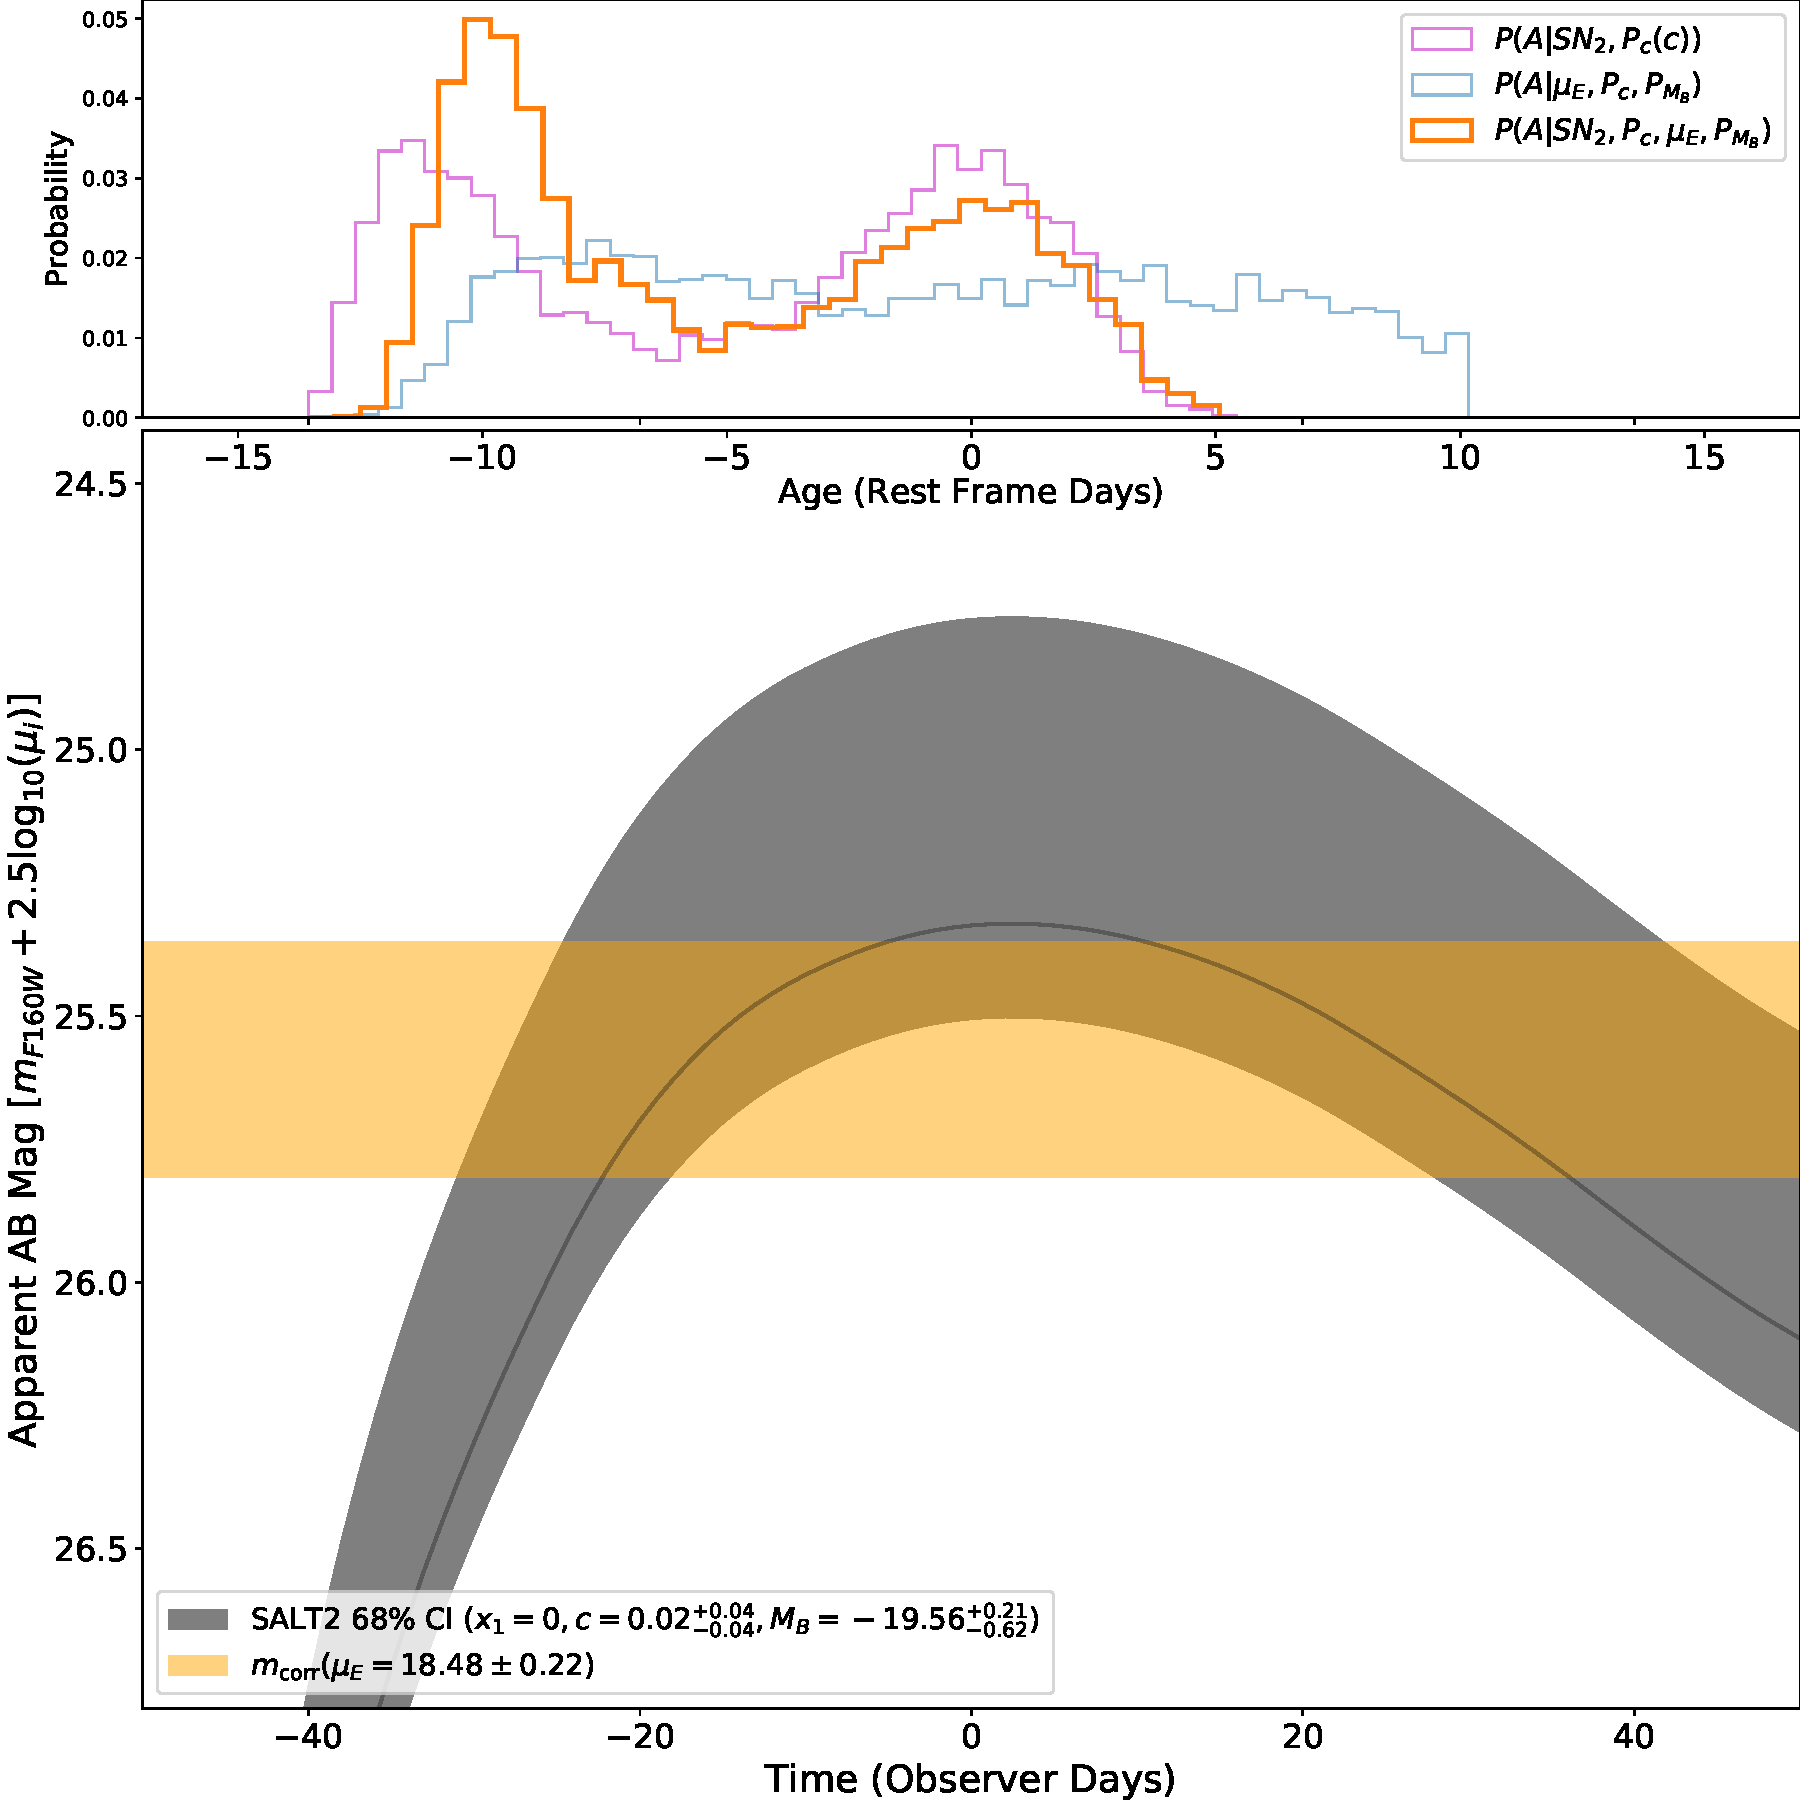
\includegraphics[width=0.45\textwidth]{Images/lightcurve_image2.pdf}
%     \caption{Light-curve-based age constraints for \SNABC image 2, using the methodology outlined in section \ref{s:lightcurves}. The upper panel shows the posterior distributions from SNTD for the age of image 2 from section \ref{s:colorcurves} (magenta), section \ref{s:lightcurves} (light blue), and the combination of both methods (orange). The grey shaded region covers the 68\% confidence interval of the best-fit SALT2 light curve, with the median model shown as a solid line. The orange shaded region shows the 1$\sigma$ range of the measured (lens-model-corrected, see table \ref{tab:time_delays}) F160W magnitude, which corresponds to a V band magnitude in the rest-frame. }
%     \label{fig:lightcurve2}
% \end{figure}

% \begin{table}[ht]
% \begin{tabular}{crrrrrrr}
    
    
%     \multicolumn{1}{c}{Model} &\multicolumn{1}{c}{$\mu_1$} & \multicolumn{1}{c}{$\mu_2$} &\multicolumn{1}{c}{$\mu_3$} &\multicolumn{1}{c}{$t_2-t_1$} & \multicolumn{1}{c}{$t_3-t_1$}& \multicolumn{1}{c}{$t_4-t_1$} & \multicolumn{1}{c}{Bayesian Evidence}\\
% \midrule
% \textit{A} & 6.324 & 9.526 & 6.879 & 180.3 & 82.7&7402.8&$-10.98\pm0.28$ \\
% \textit{B} & 6.281 & 9.923 & 7.472 & 184.4 & 85.3&7034.9&$-10.21\pm0.27$ \\
% \textit{C} &8.942  & 18.48 & 13.257 & 103.6 & 50.2&5876.8&$-6.91\pm0.22$ \\
% \textit{D} & 8.699 & 18.069 & 12.719 & 108.3 & 53.7&6020.5&$-7.78\pm0.24$ \\
% \textit{E} & 3.907 & 7.381 & 5.020 & 101.4 & 19.3&7760&$-6.95\pm0.2$ \\
% \end{tabular}
% \caption{\label{tab:model_evidence}Predicted lensing observables and Bayesian evidence for the five lens model variants investigated in this work. The Bayesian evidences in the final column are calculated by comparison to the observed photometry, using a coarse (100 live points) nested sampling fit, which helps identify models C and E as preferred over A,B, and D. We then implement a finer nested sampling fit (1,000 live points), and find that in fact model E is preferred at $>3\sigma$ ($Z_C=-7.25\pm0.07, \ Z_E=-   7.00\pm0.06$).}
% \end{table}

%\section*{Supplementary Text}

\subsection*{Final Inferred Time Delays and the \SNABC Light Curve}

Our final age constraints for each SN image are a joint posterior between the parameter estimates from color-curve fitting (lens model independent) and light curve fitting (lens model dependent), resulting in the final time delays and uncertainties reported in table \ref{tab:time_delays} of the main text. Using these measured time delays, we can create a reconstructed form of the intrinsic light curve (Fig. \ref{fig:full_lightcurve}) and color curve (Fig. \ref{fig:full_colorcurve}) of \SNABC.


The final posterior distributions for images 2 and 3 are extremely bi-modal due to a degeneracy that cannot be broken by single epoch photometry, corresponding to a double-peaked intrinsic luminosity posterior for \SNABC (Fig. \ref{fig:corner_combined}). If this degeneracy can be broken with the precise photometry expected for the final image of Requiem, then the final time delay uncertainty for \SNABC could be below $0.1\%$.

% updated to SNTD fits and new fluxes
\begin{figure*}
    \centering
    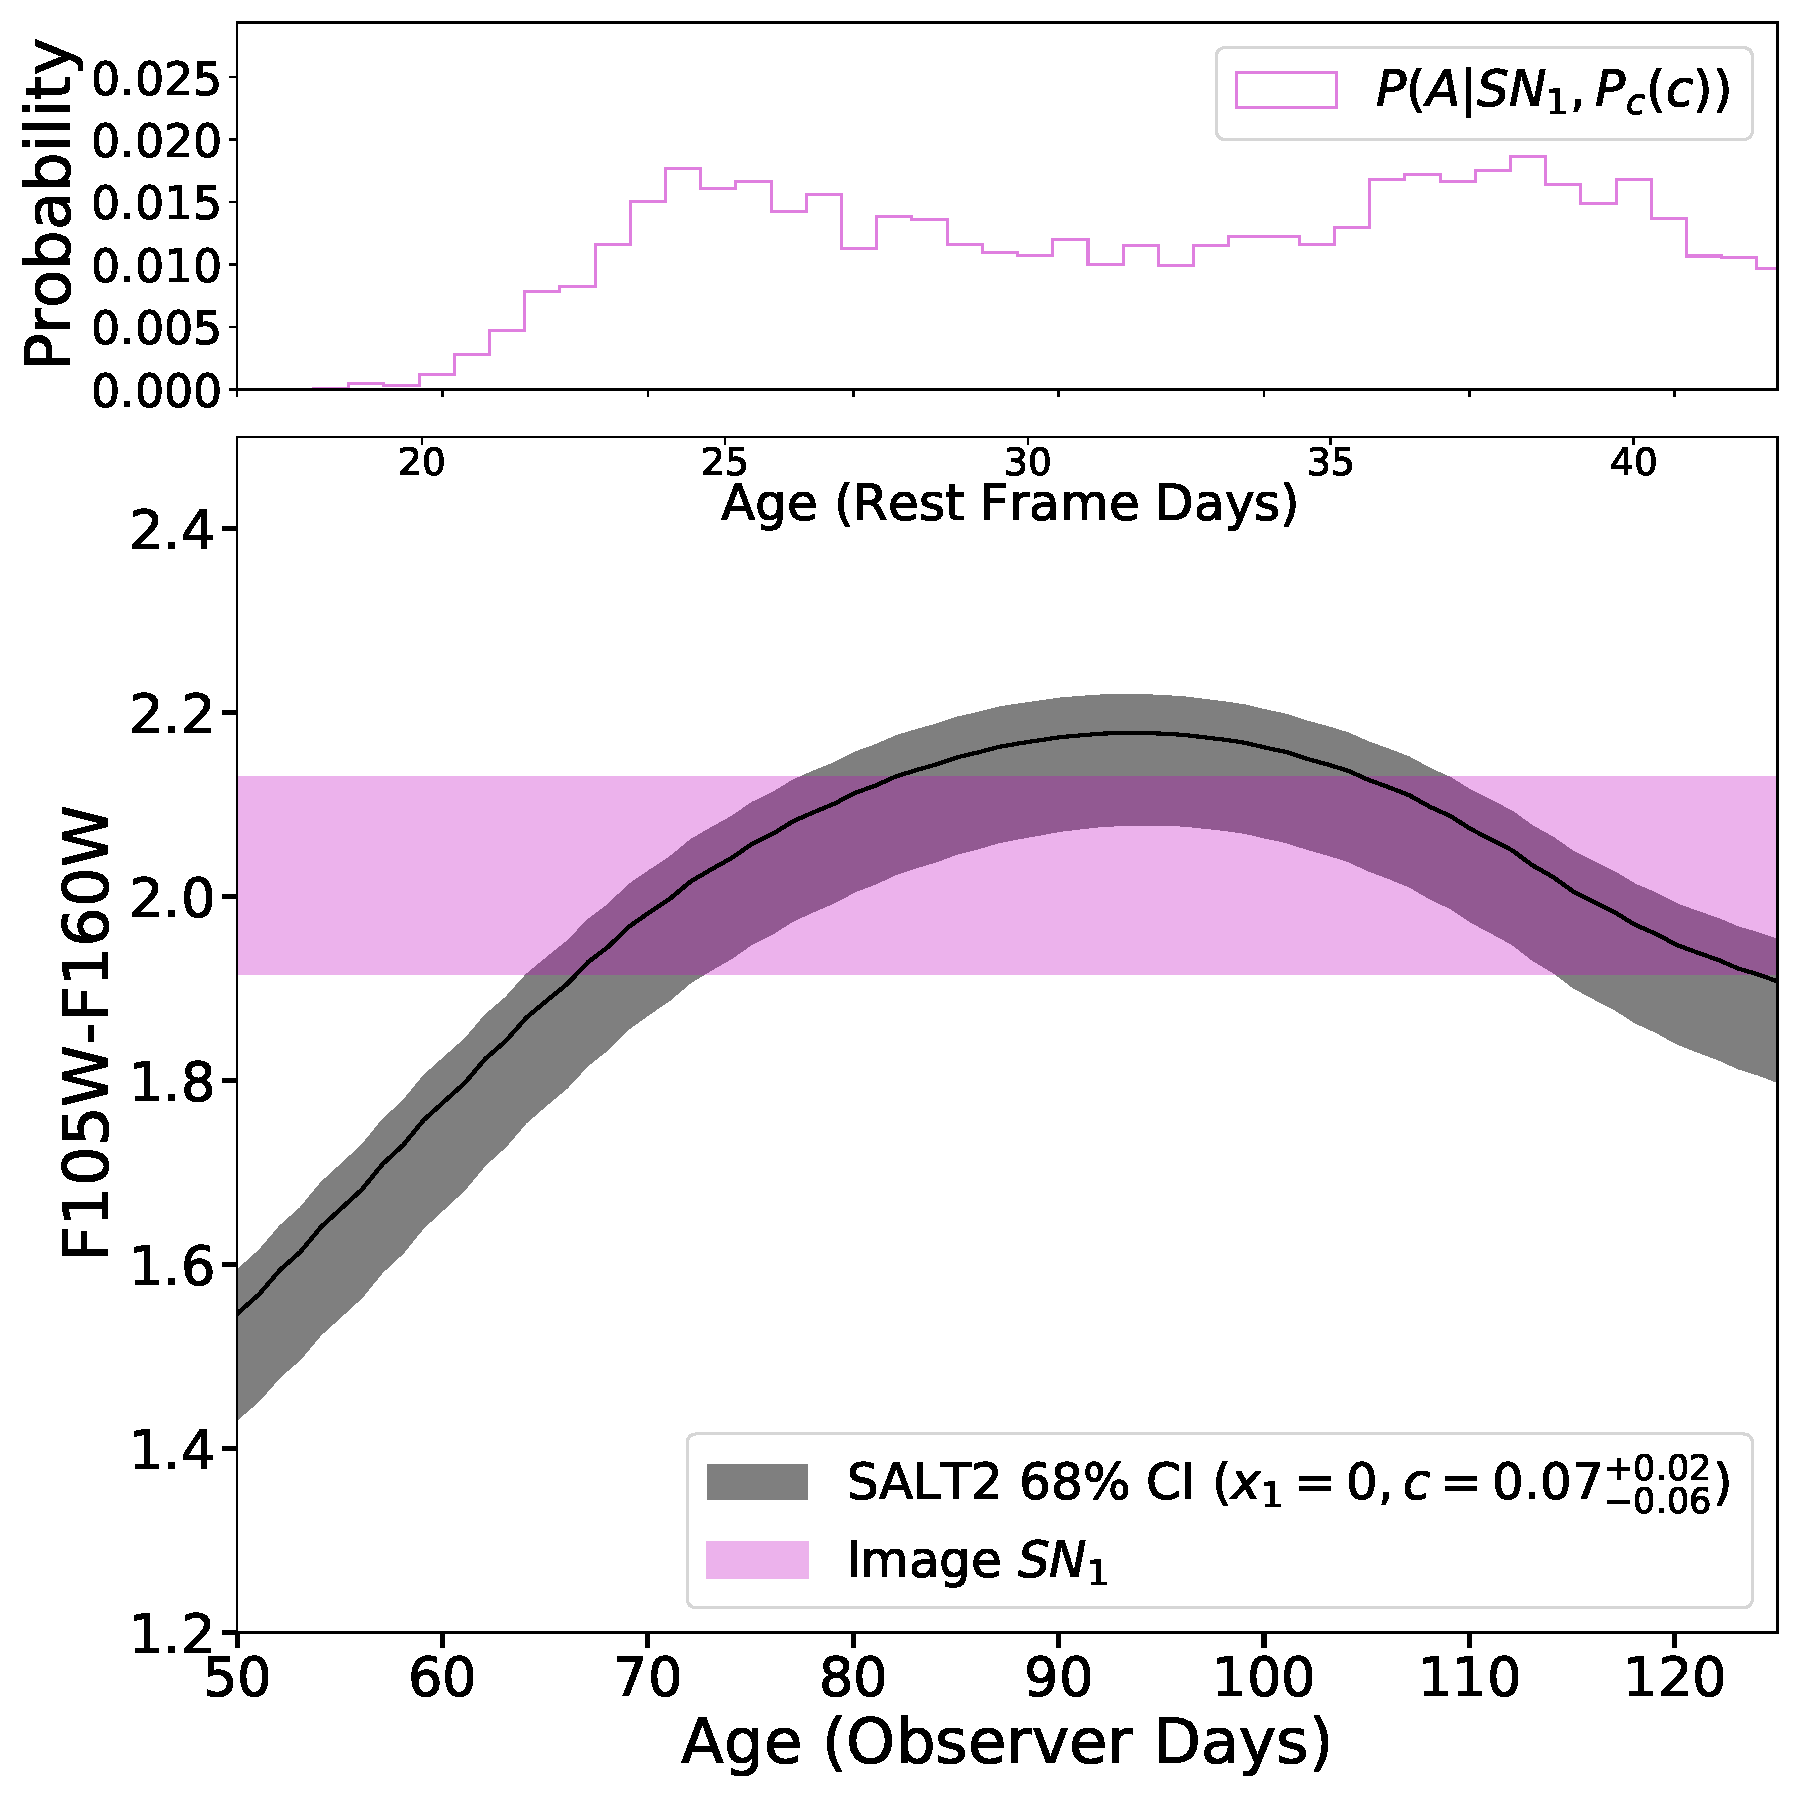
\includegraphics[width=0.49\textwidth]{Paper/Figures/colorcurve_image1.pdf}
    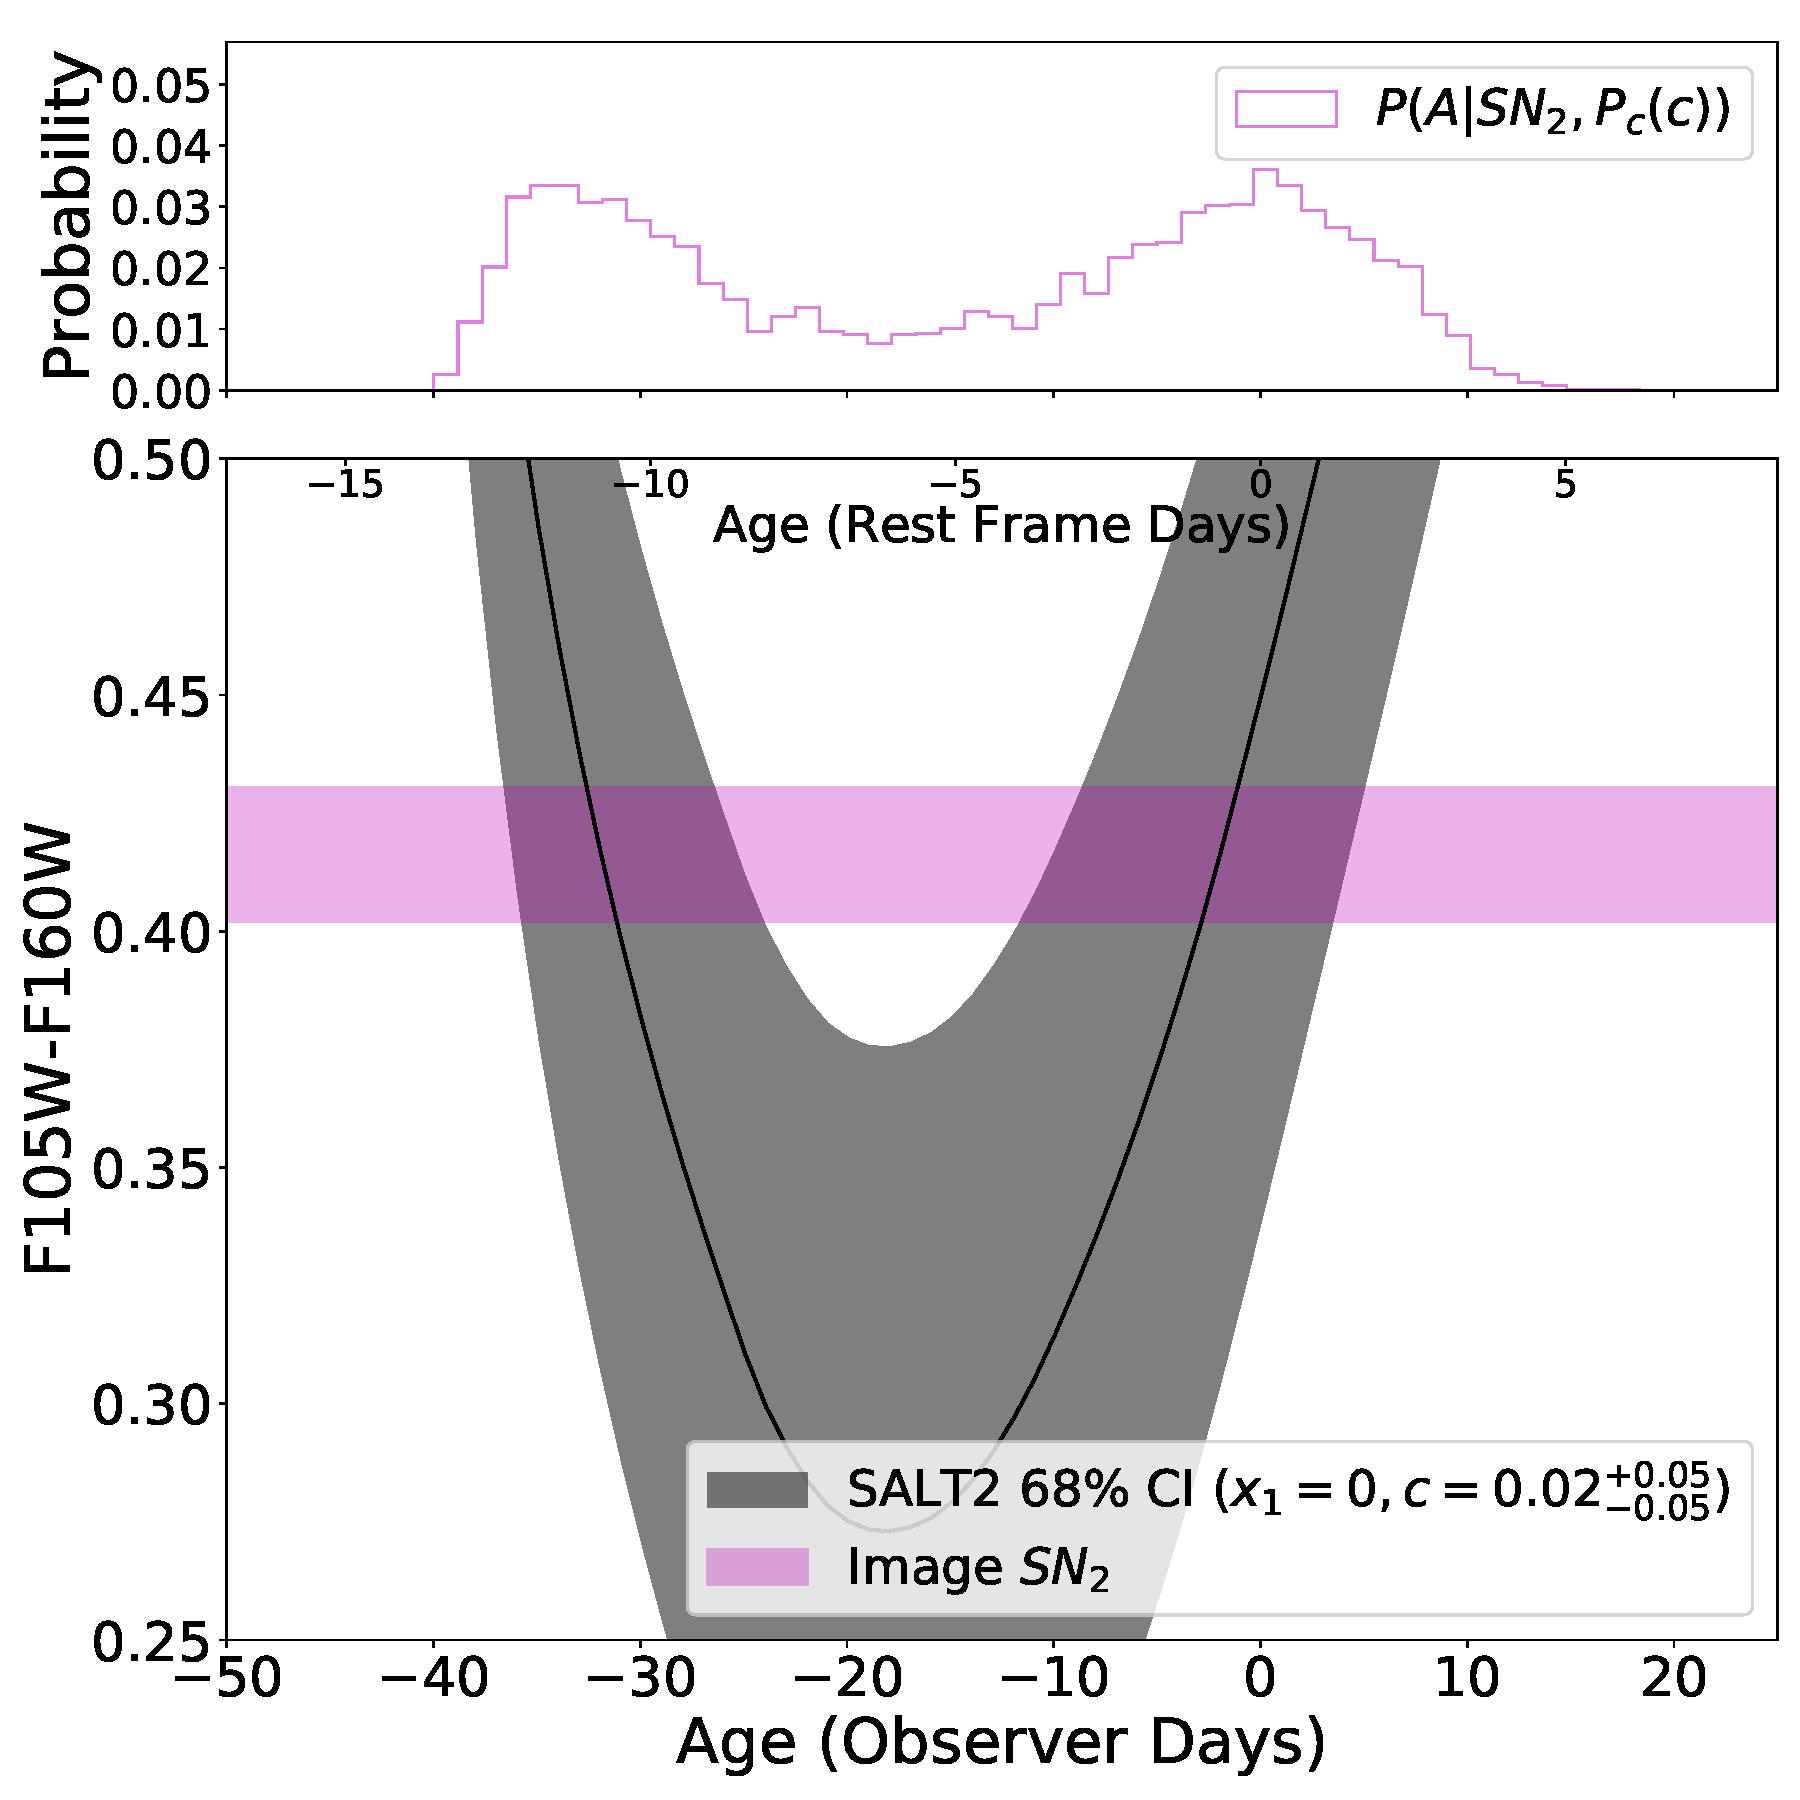
\includegraphics[width=0.49\textwidth]{Paper/Figures/colorcurve_image2.pdf}
    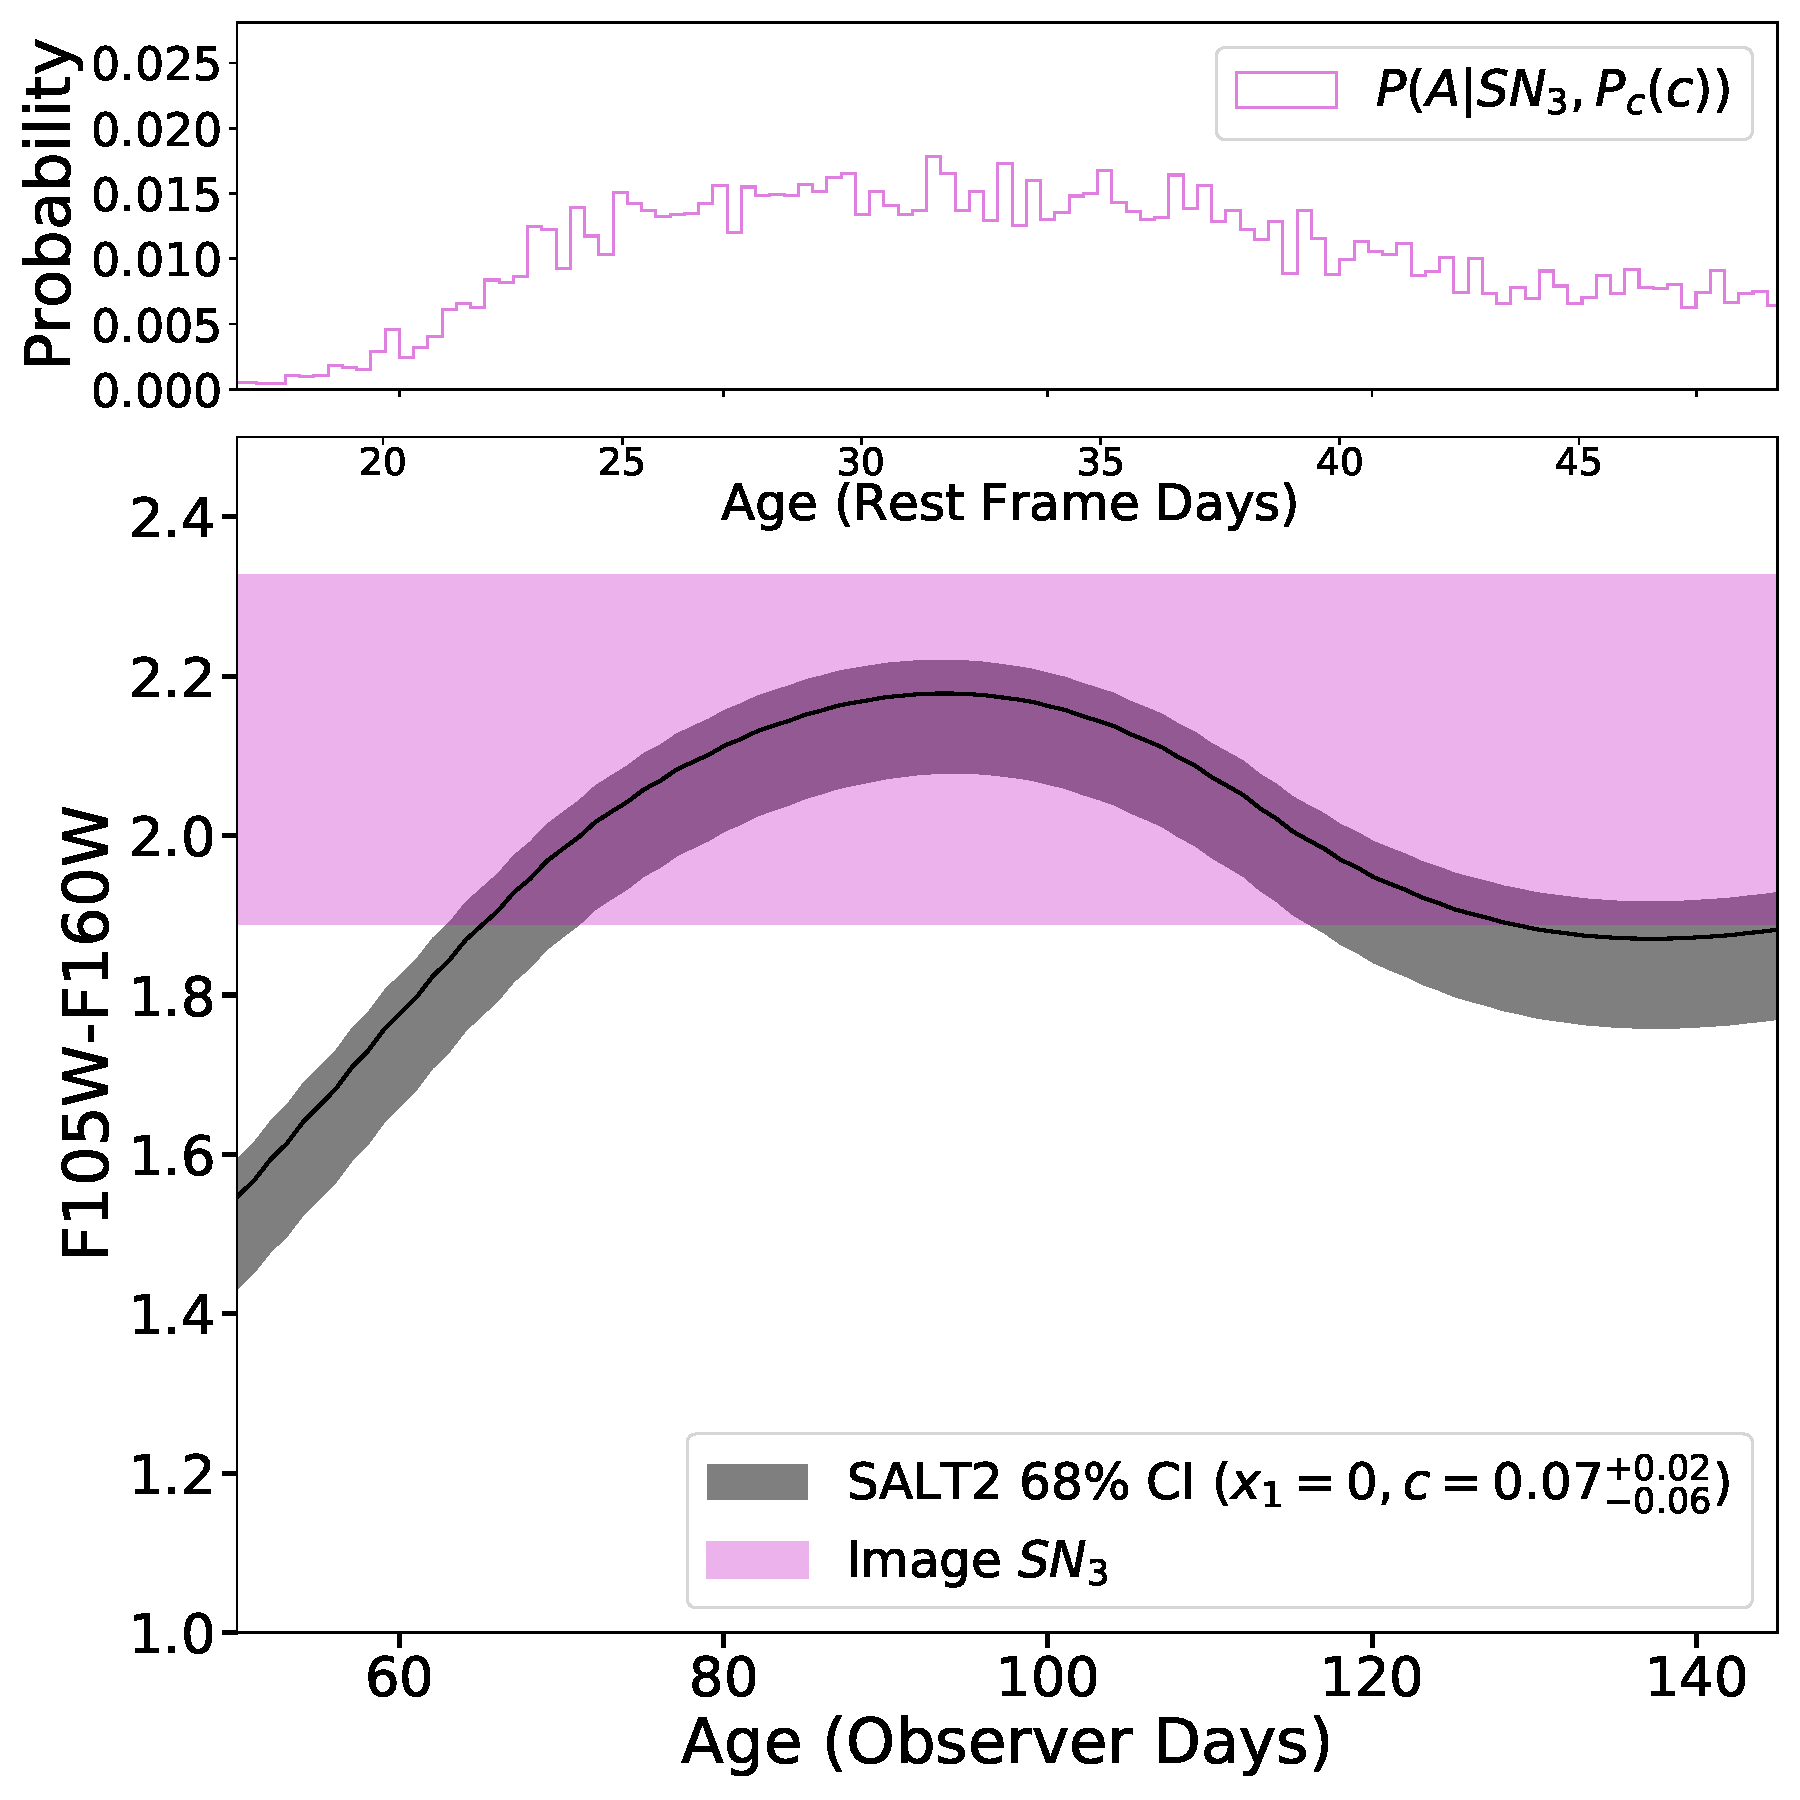
\includegraphics[width=0.49\textwidth]{Paper/Figures/colorcurve_image3.pdf}
    \caption{Color-based age constraints for \SNABC image 1 (upper \replaced[id=r1]{left}{right}), image 2 (upper right), and image 3 (bottom center), using the methodology outlined in the \textit{Color Curve Age Constraints} section. The upper panel of each figure shows the posterior for the age of each image from SNTD, using a prior on the SALT2 color parameter (c) based on known population characteristics of SNIa. The effect of adding this prior is slight, with no significant deviation from the best-fit value of c ($0.02^{+0.04}_{-0.05}$). The grey shaded region covers the 68\% confidence interval of the best-fit SALT2 color curve, with the median model shown as a solid line. The magenta shaded region shows the 1$\sigma$ range of the measured F105W-F160W color, which corresponds to a $U-V$ color in the rest-frame.}
    \label{fig:colorcurves}
\end{figure*}



\begin{figure*}
    \centering
    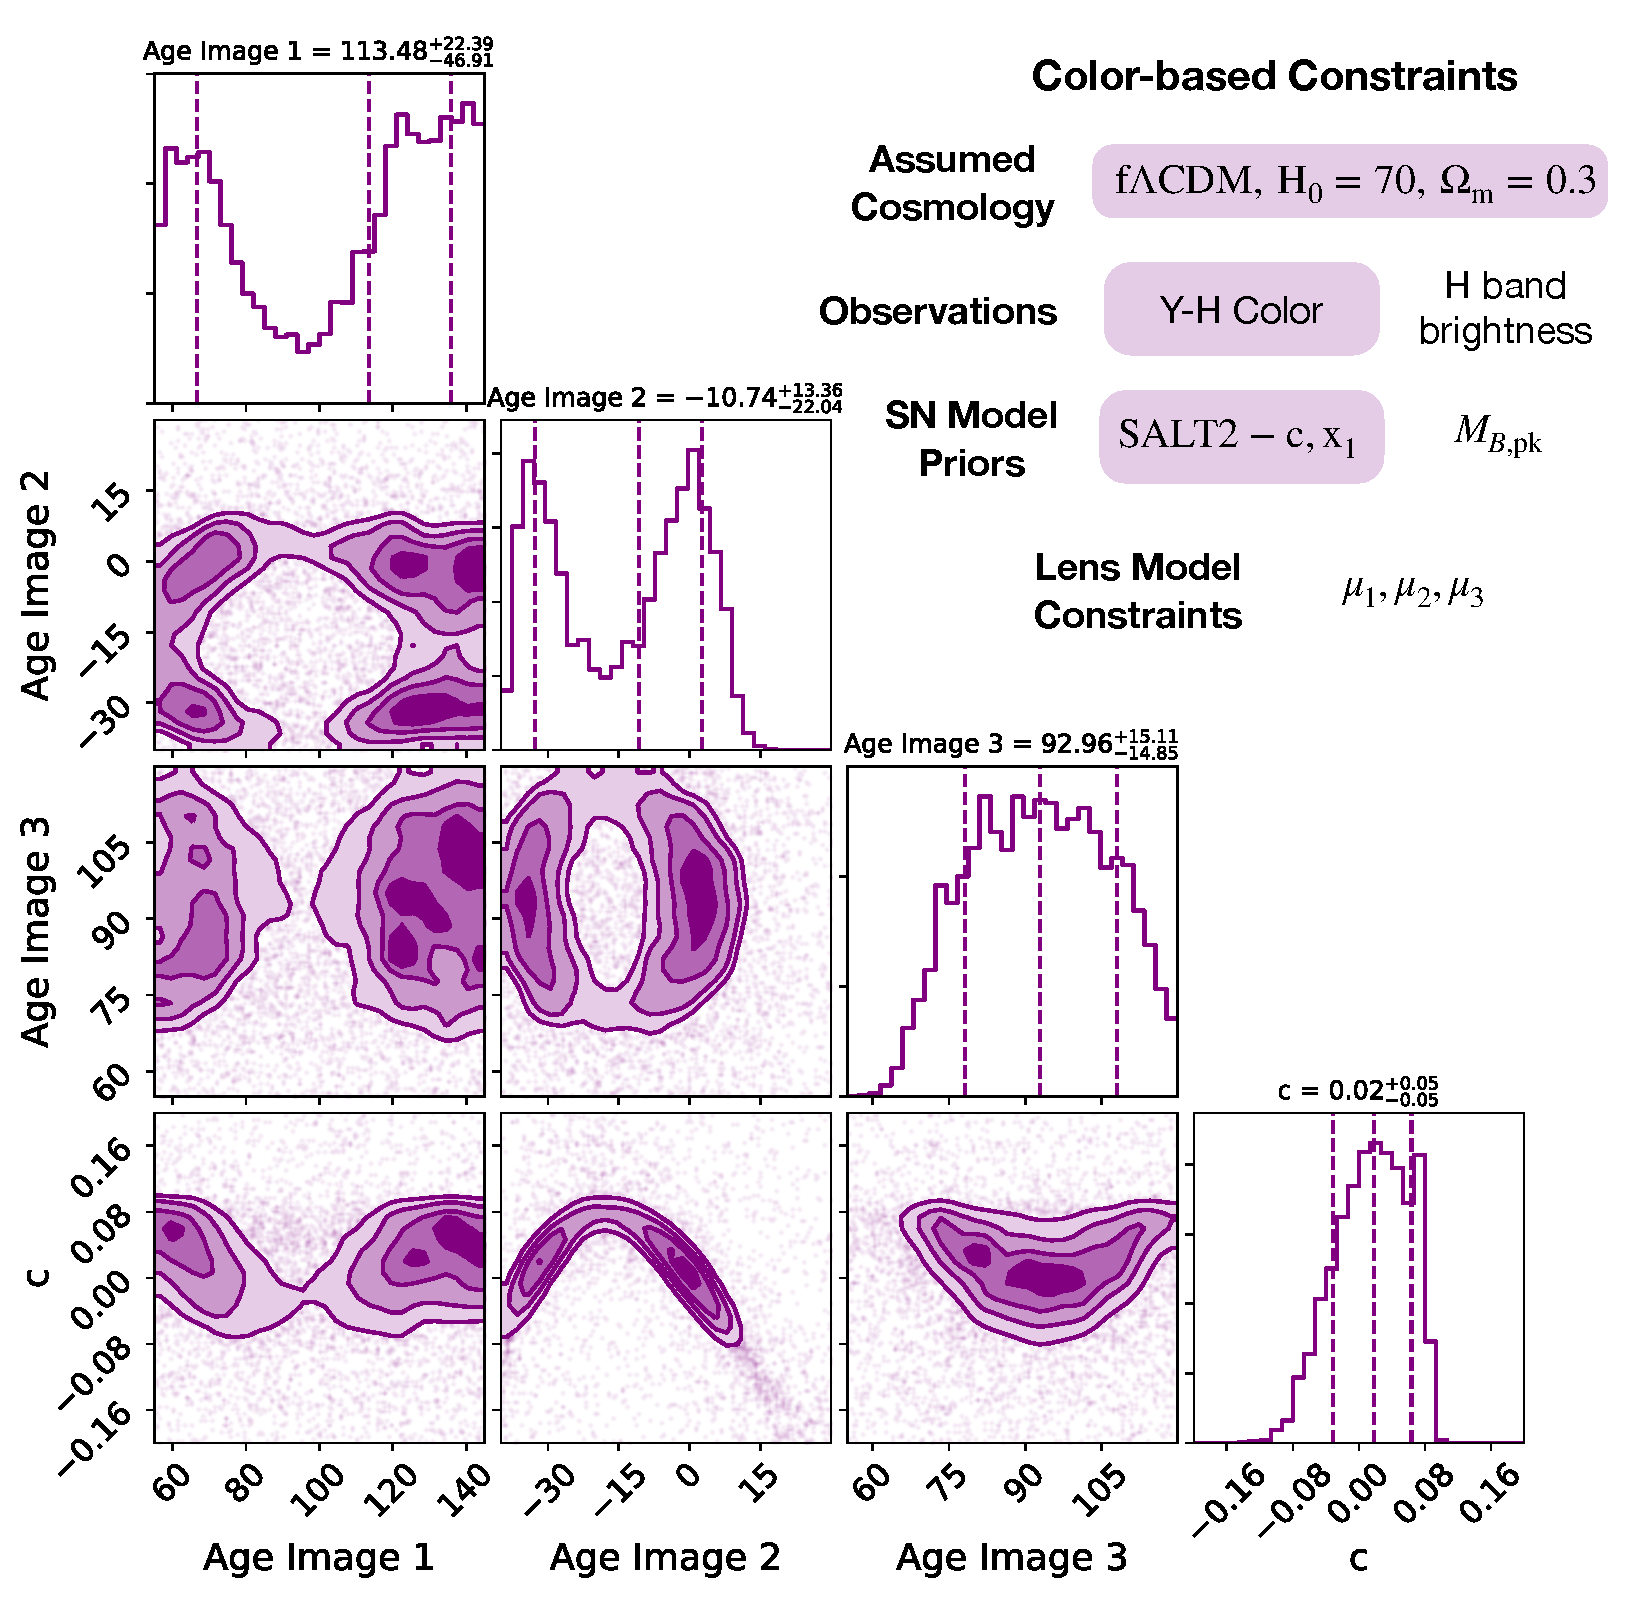
\includegraphics[width=0.9\textwidth]{Paper/Figures/corner_color_curve_fit_with_c_prior_labels}
%    corner_color_curve_fit_with_c_prior.pdf}
    \caption{The marginalized and joint posterior distributions for the color curve age constraints measured in this analysis. We use a weak prior on the SALT2 color parameter ($c$), and set the SALT2 stretch parameter ($x_1$) to 0. This method is fully independent of lens modeling.  The table in the upper right lists all 
    priors, observations, and lens model information
    used for SN age estimates in this work.  
    Only the highlighted 
    components were used for the constraints shown here.}
    \label{fig:corner_cfit}
\end{figure*}

% updated to SNTD fits and new fluxes
\begin{figure*}
    \centering
    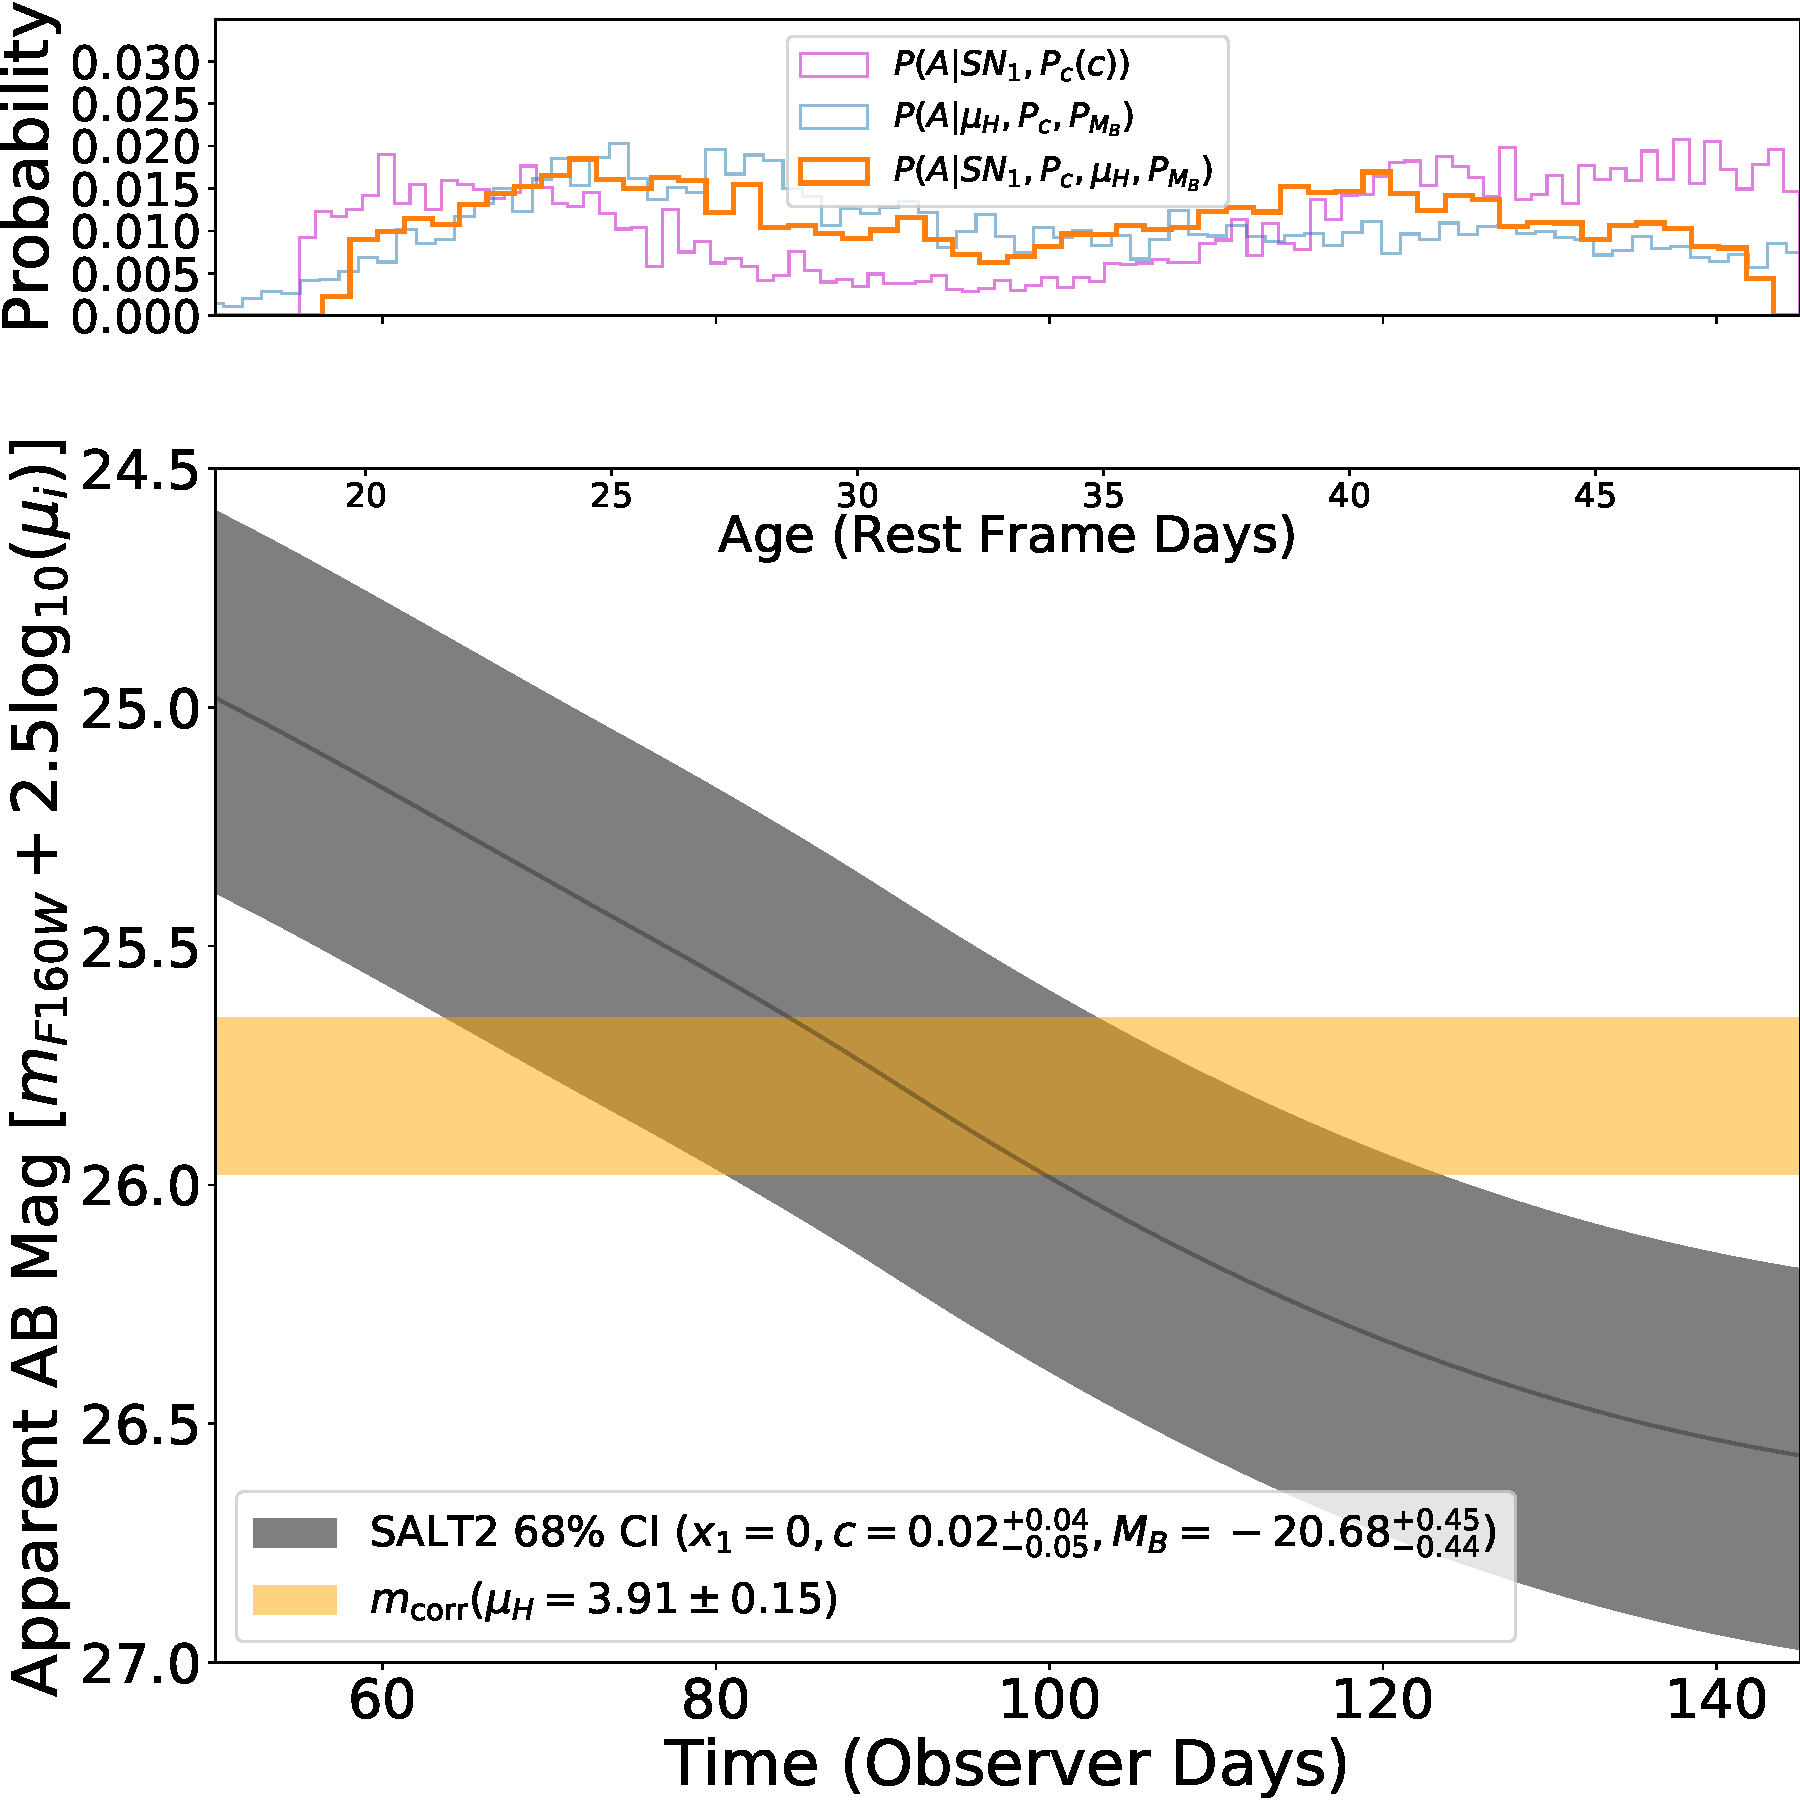
\includegraphics[width=0.49\textwidth]{Paper/Figures/lightcurve_image1.pdf}
    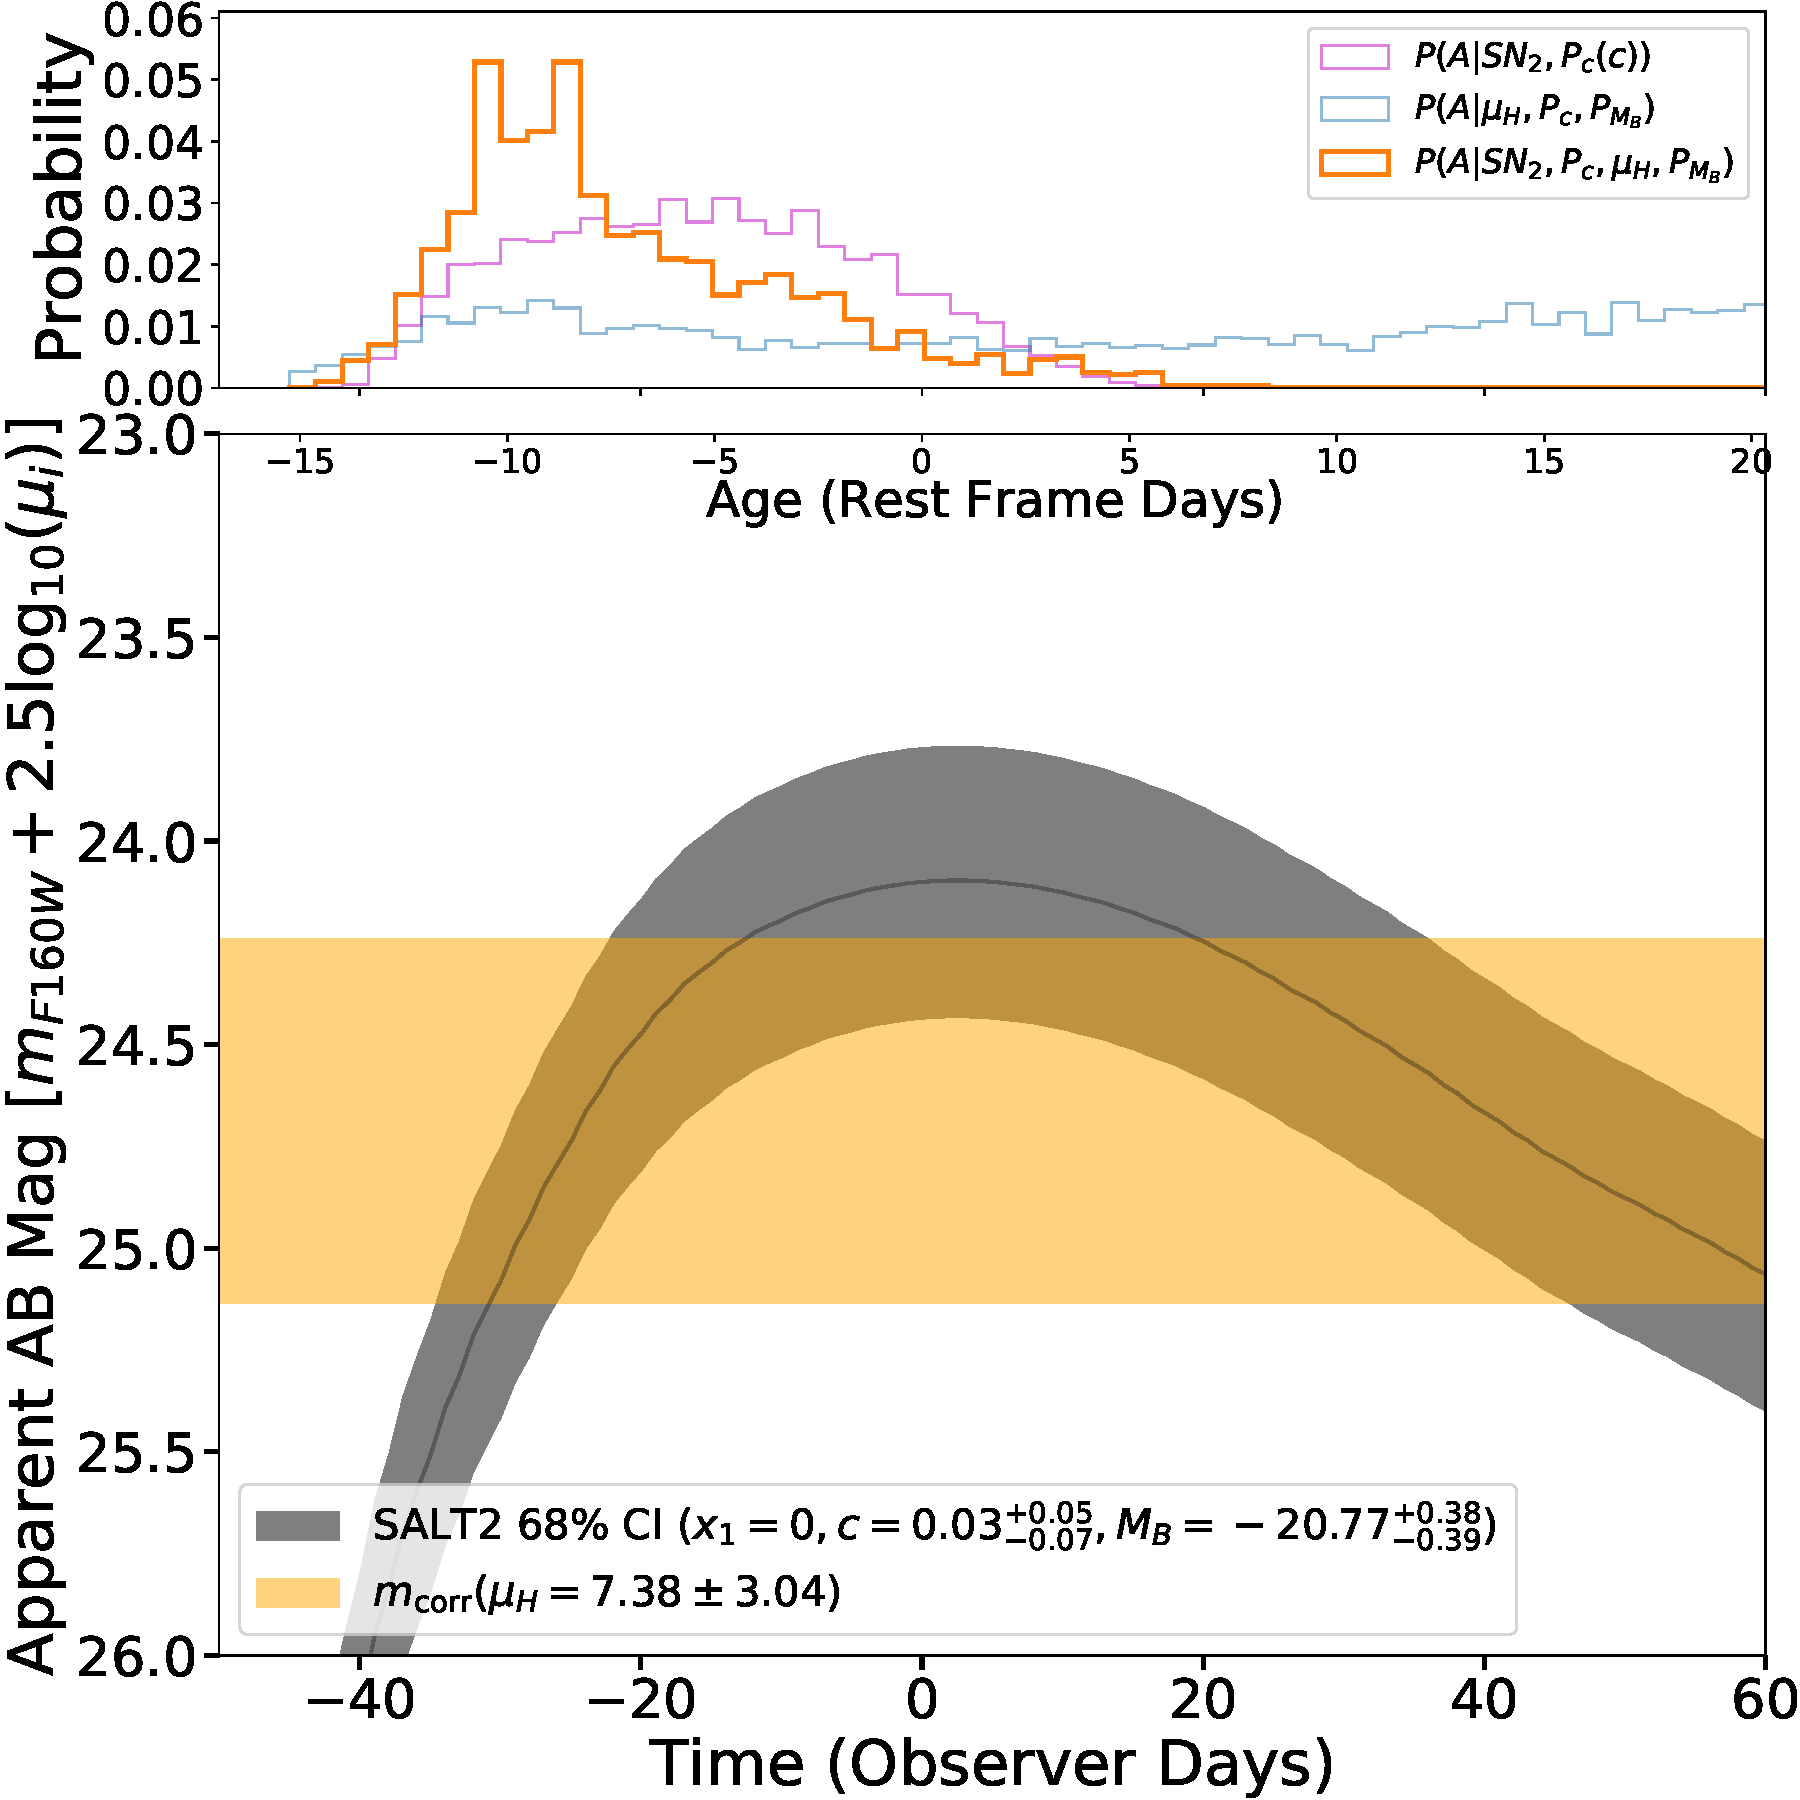
\includegraphics[width=0.49\textwidth]{Paper/Figures/lightcurve_image2.pdf}
    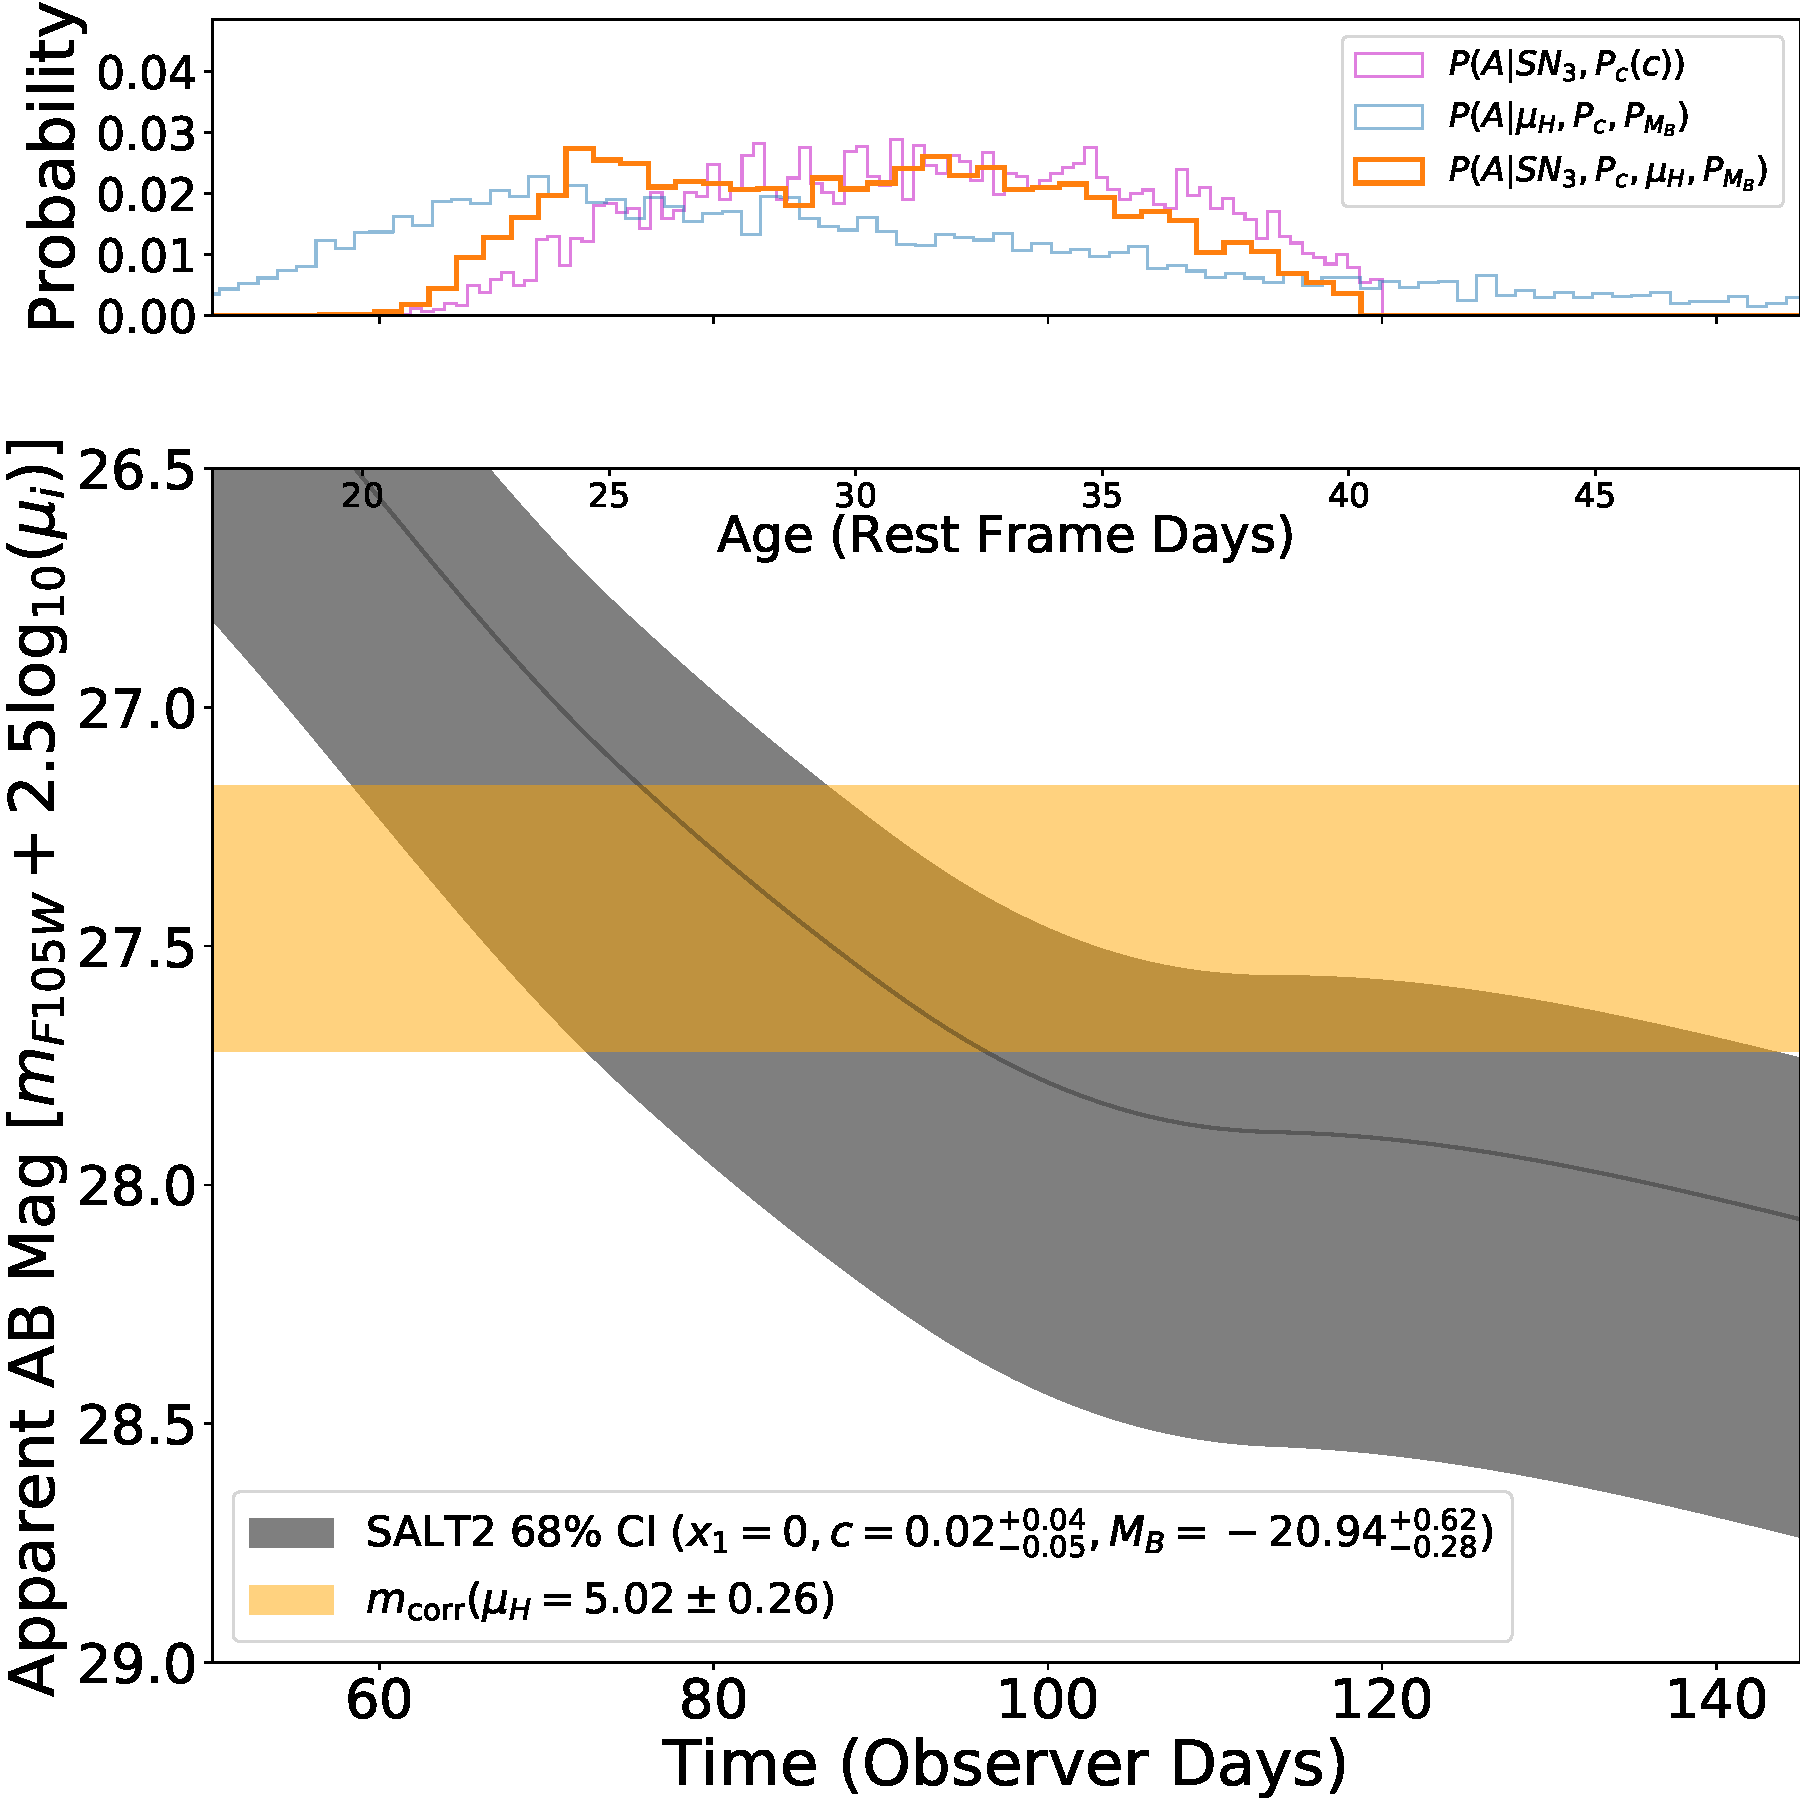
\includegraphics[width=0.49\textwidth]{Paper/Figures/lightcurve_image3.pdf}
    \caption{Light-curve-based age constraints for \SNABC image 1 (upper \replaced[id=r1]{left}{right}), image 2 (upper right), and image 3 (bottom center), using the methodology outlined in the \textit{Light Curve Age Constraints} section. The upper panel in each figure shows the posterior distributions from SNTD for the age of each image that is independent of the lens model (magenta, figure \ref{fig:colorcurves}), using lens model E (light blue), and the combination of both methods (orange). The grey shaded region covers the 68\% confidence interval of the best-fit SALT2 light curve, with the median model shown as a solid line. The orange shaded region shows the 1$\sigma$ range of the measured (lens-model-corrected, see table \ref{tab:time_delays}) F160W magnitude, which corresponds to a V band magnitude in the rest-frame.}
    \label{fig:lightcurves}
\end{figure*}


%\begin{figure*}
%    \centering
%    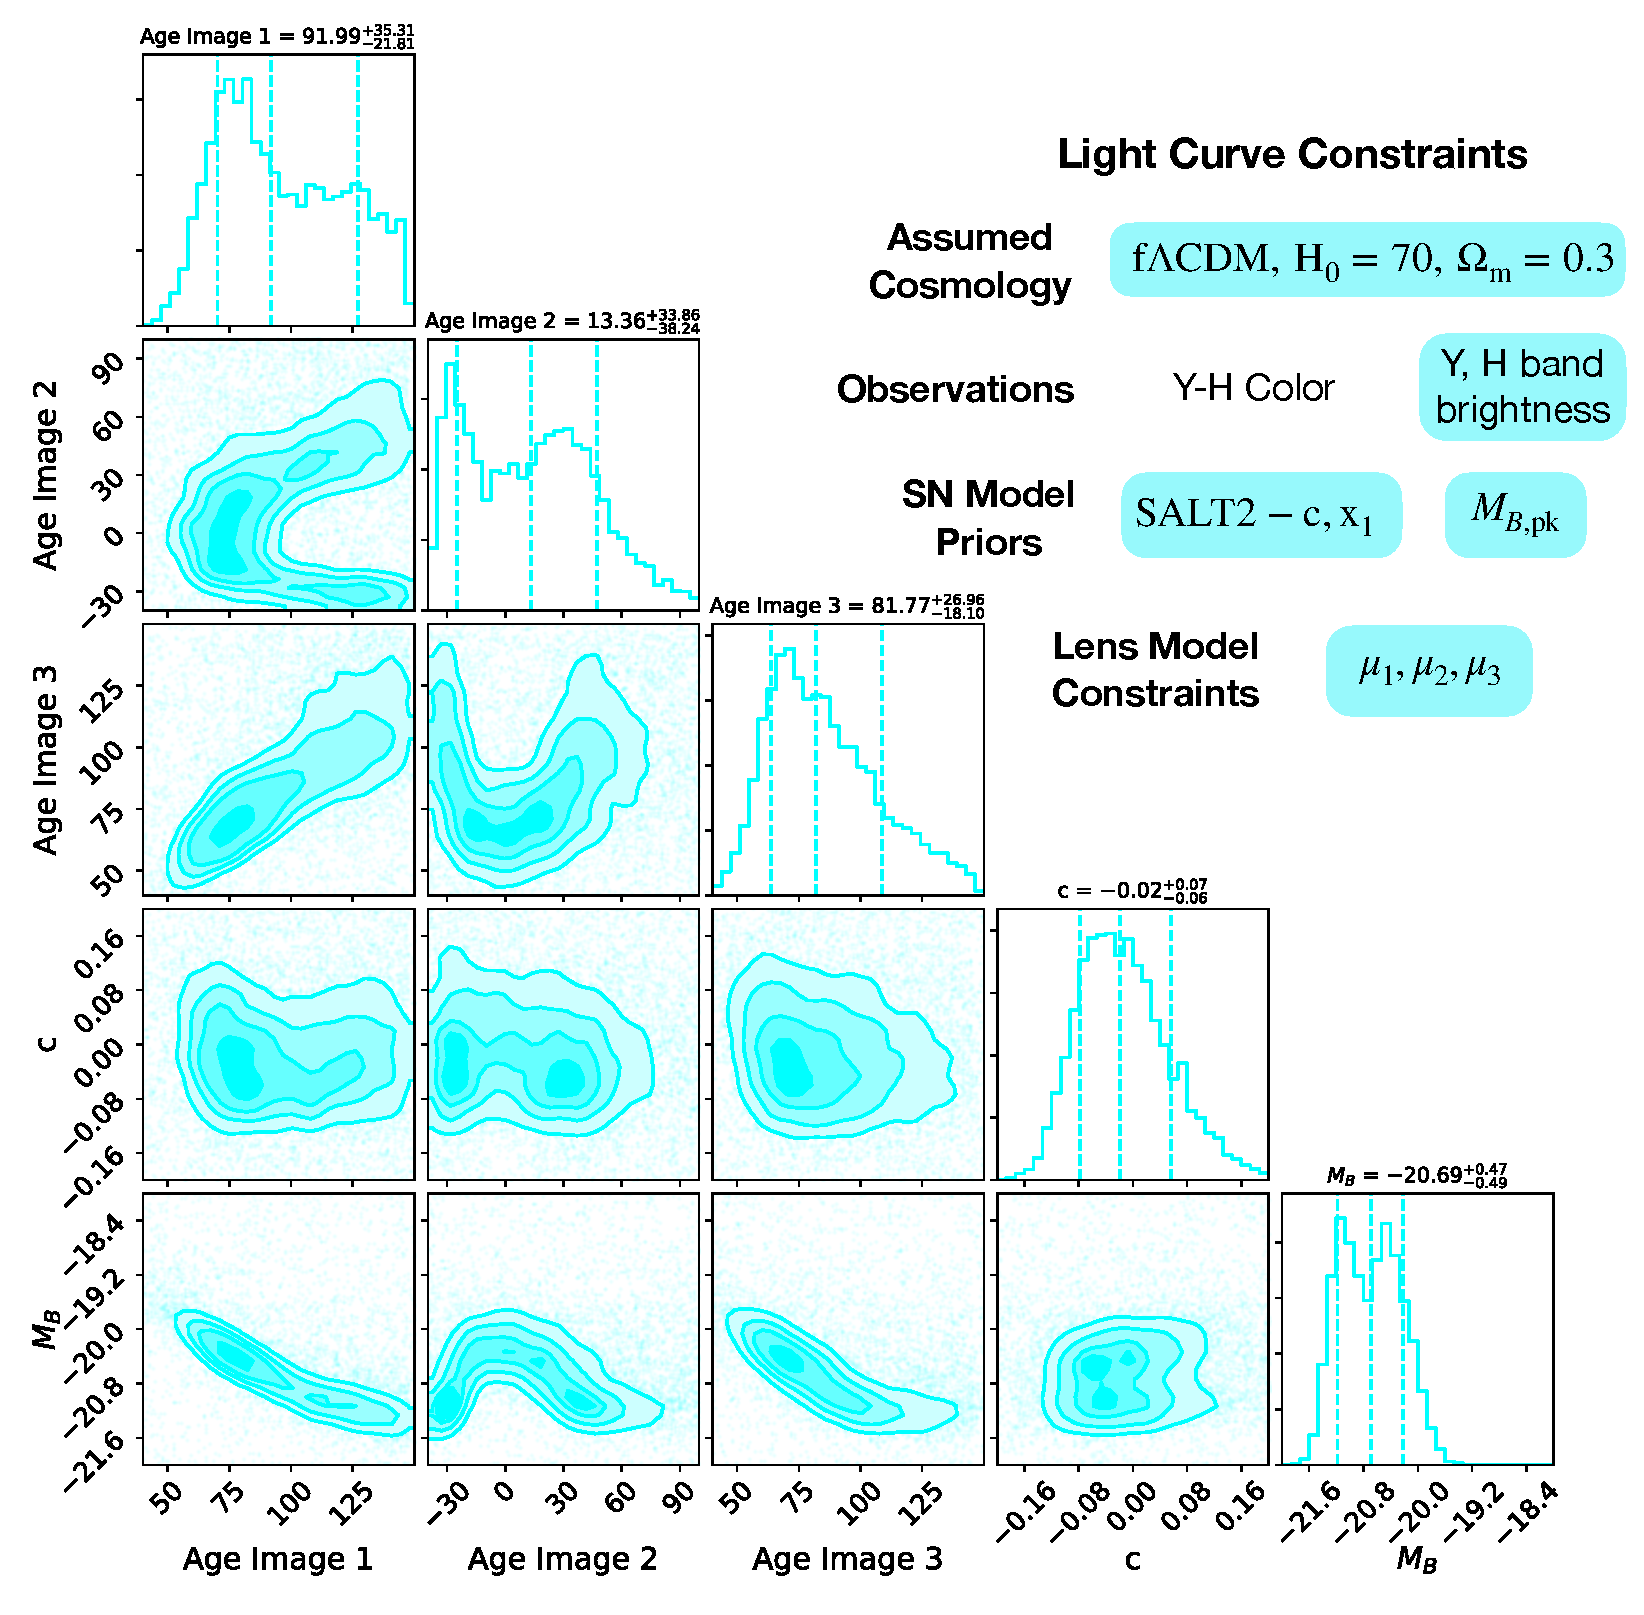
\includegraphics[width=0.9\textwidth]{Paper/Figures/lc_modelH_corner_labels.pdf}
%    \caption{The marginalized and joint posterior distributions for the light curve age constraints measured in this analysis. We use lens model E to de-magnify each image and fit the corrected apparent magnitudes. This fit includes weak priors on the absolute magnitude of a SNIa ($M_B$) and the SALT2 color parameter ($c$), and sets the SALT2 stretch parameter ($x_1$) to 0.
%     The table in the upper right lists all 
%    priors, observations, and lens model information
%    used for SN age estimates in this work.  
%    Only the highlighted 
%    components were used for the constraints shown here.
%    }
%    \label{fig:corner_modelE}
%\end{figure*}
\begin{figure*}
    \centering
    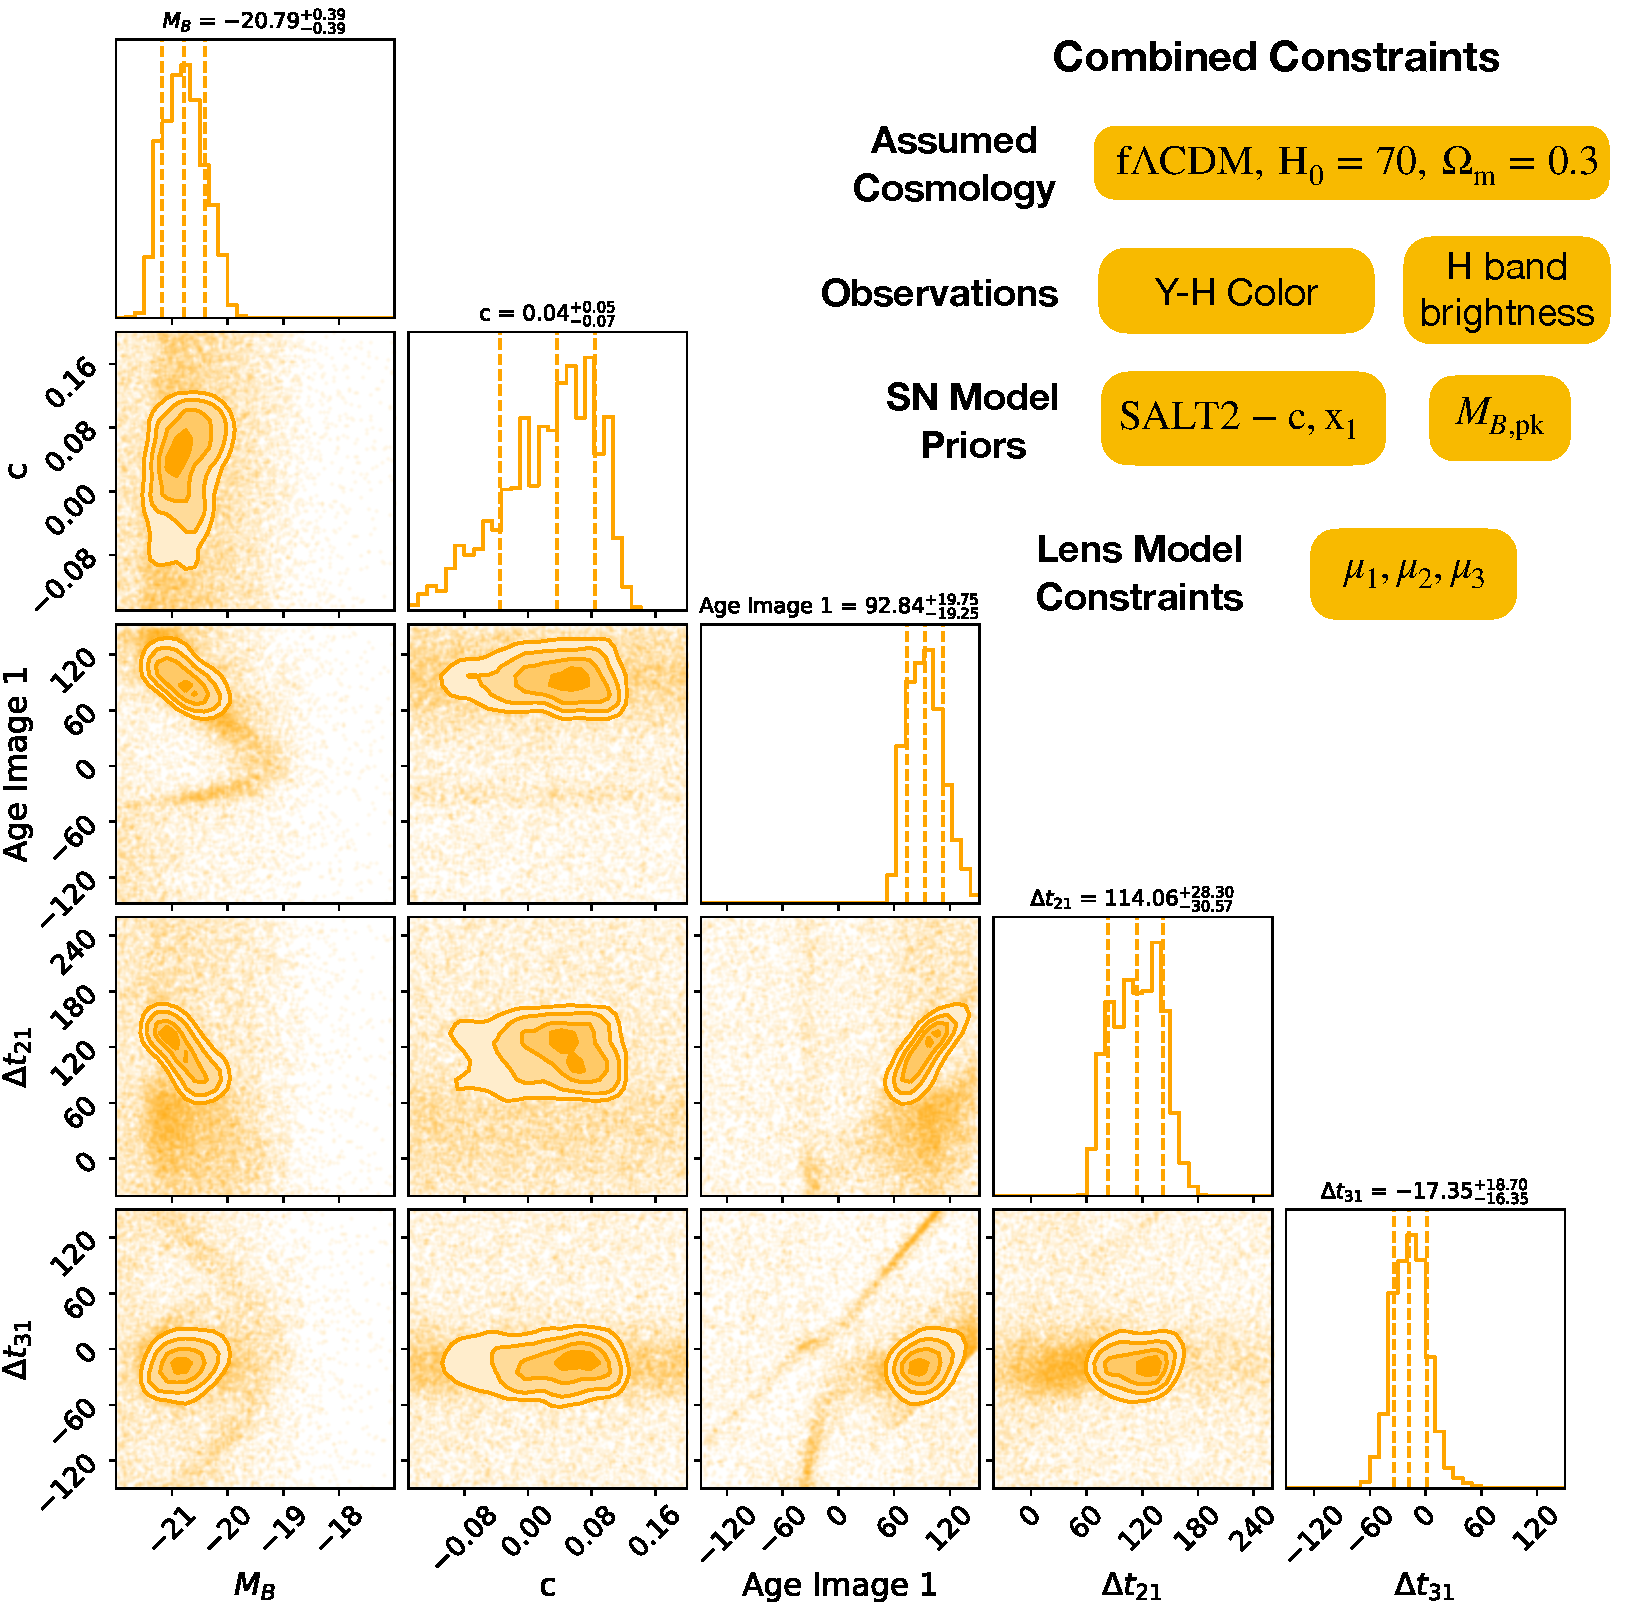
\includegraphics[width=0.9\textwidth]{Paper/Figures/lc_modelE_color_corner_labels}
    \caption{The marginalized and joint posterior distributions for the final age constraints measured in this analysis. We use the color curve posterior as the prior for light curve fitting with lens model E, and include weak priors on the absolute magnitude of a SNIa ($M_B$) and the SALT2 color parameter ($c$), and set the SALT2 stretch parameter ($x_1$) to 0.}
    \label{fig:corner_combined}
\end{figure*}
% updated to SNTD fits and new fluxes
\begin{figure}[htp]
    \centering
    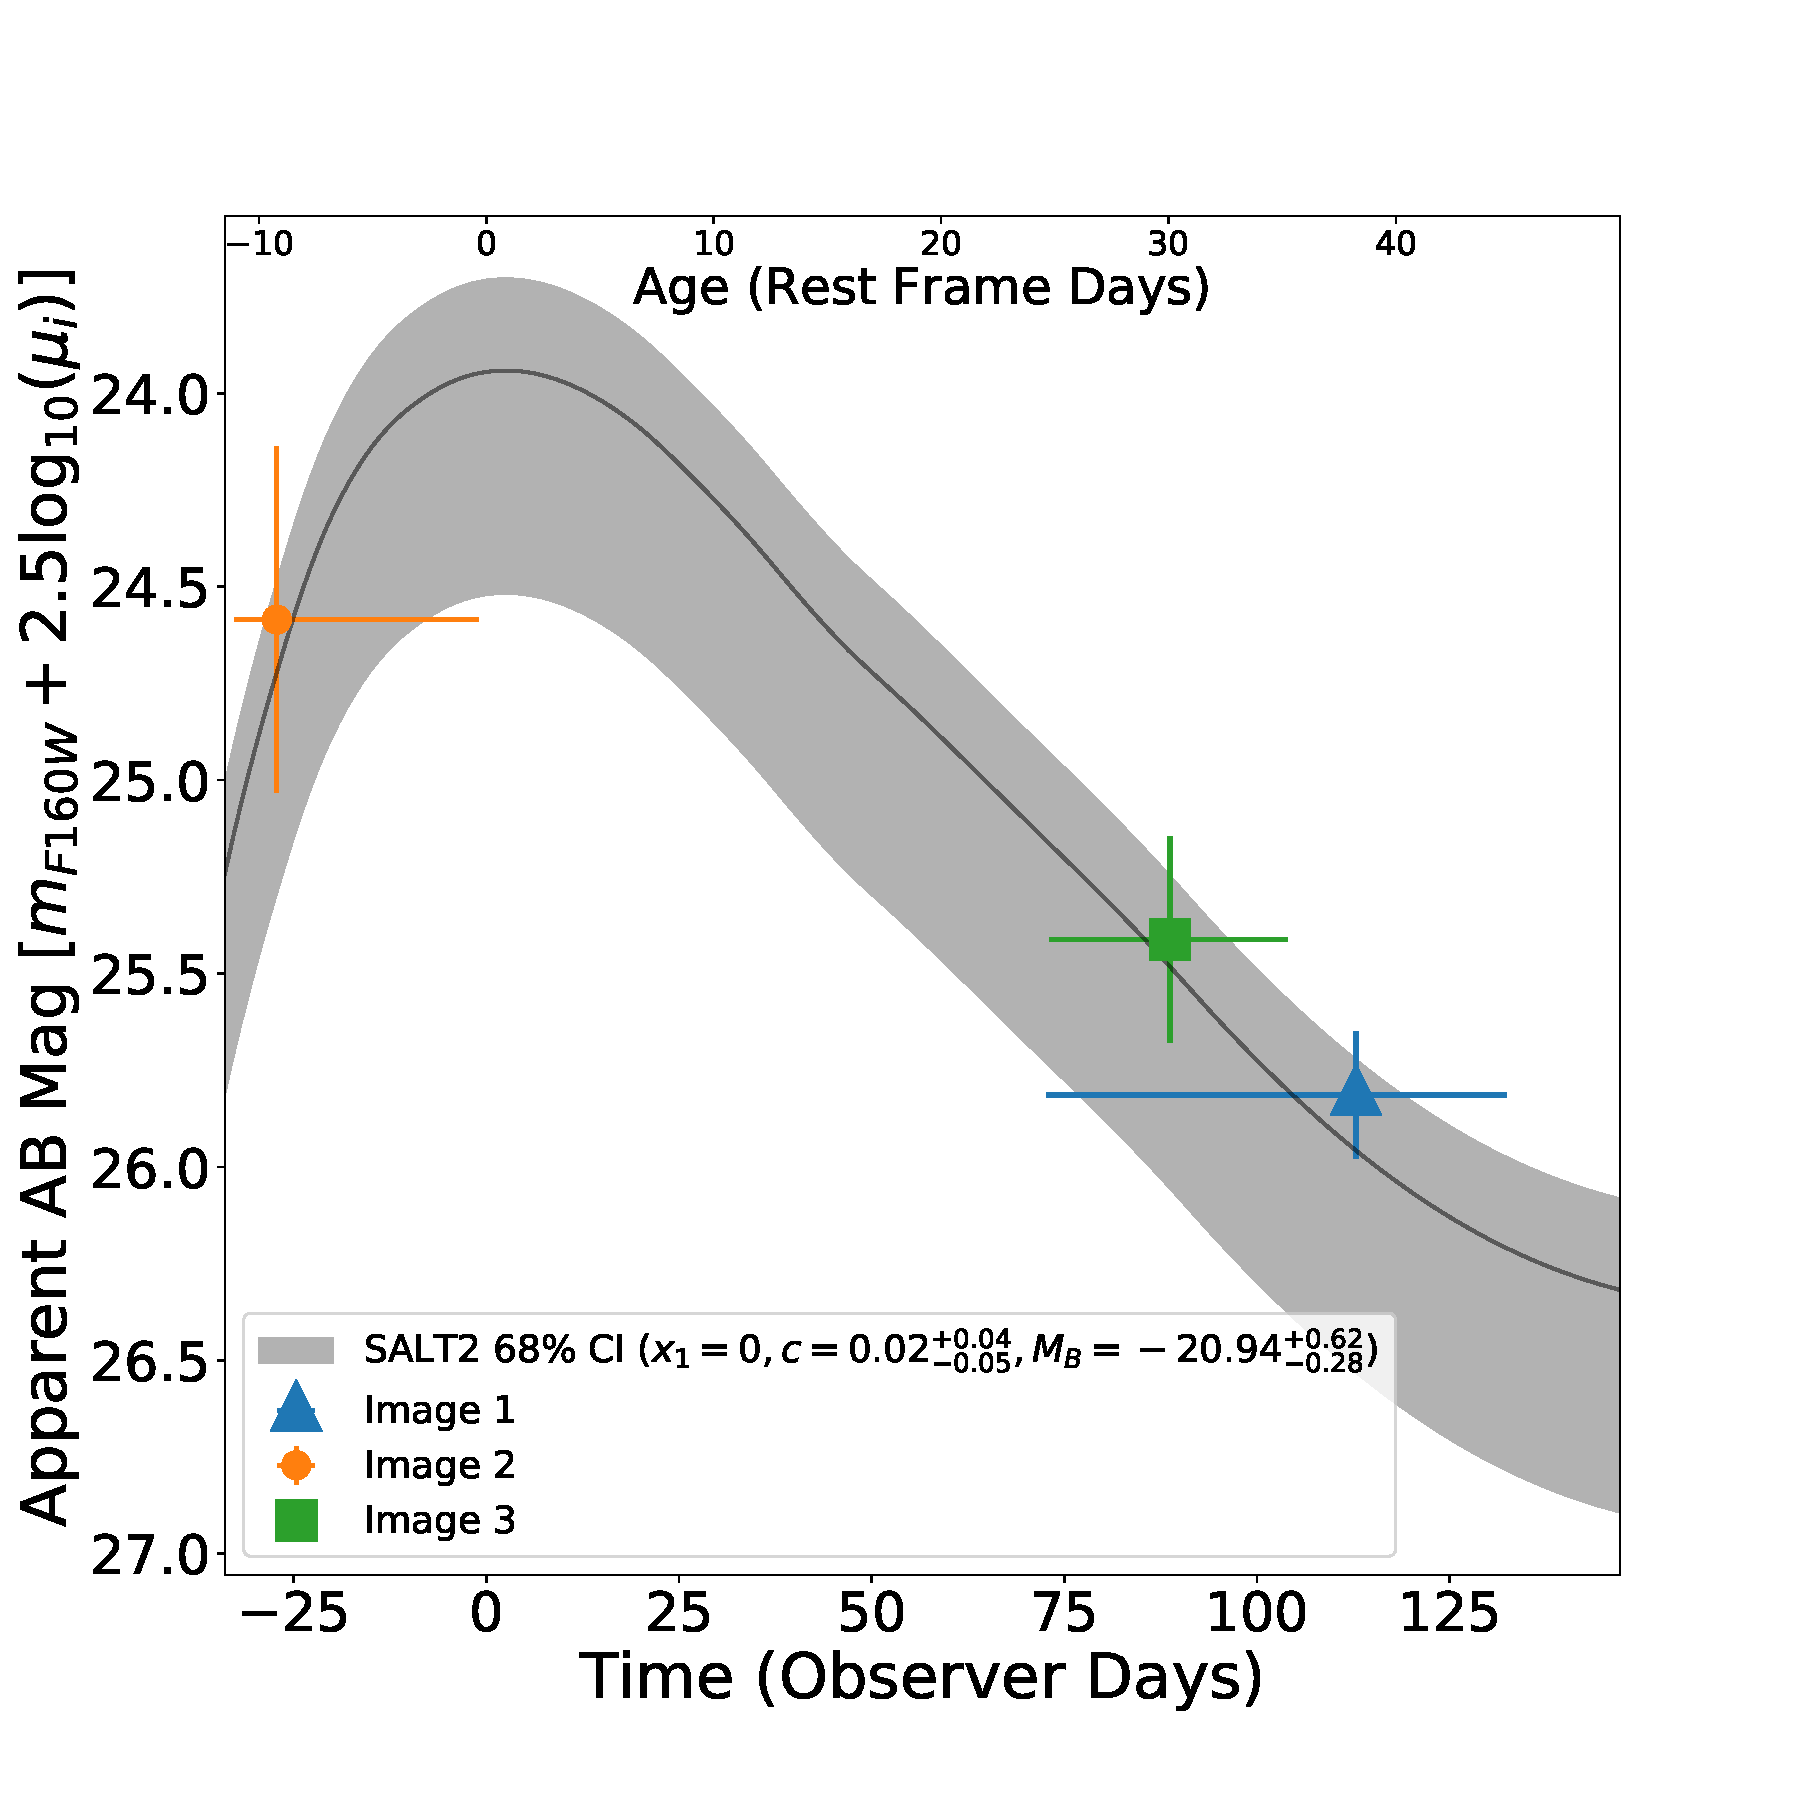
\includegraphics[width=0.6\textwidth]{Paper/Figures/full_lightcurve.pdf}
    \caption{\label{fig:full_lightcurve}The reconstructed light curve for \SNABC. The grey shaded region covers the 68\% confidence interval of the best-fit SALT2 color curve, with the median model shown as a solid line. Observed photometric data are shown as colored markers.   The error bars on each data point represent the photometric +lens model magnification (y-dimension) and time delay (x-dimension) uncertainties. These constraints are obtained using the joint posterior of the color curve and light curve methods described above, and are dependent upon lens model E.}
\end{figure}
% updated to SNTD fits and new fluxes
\begin{figure}[hbp]
    \centering
    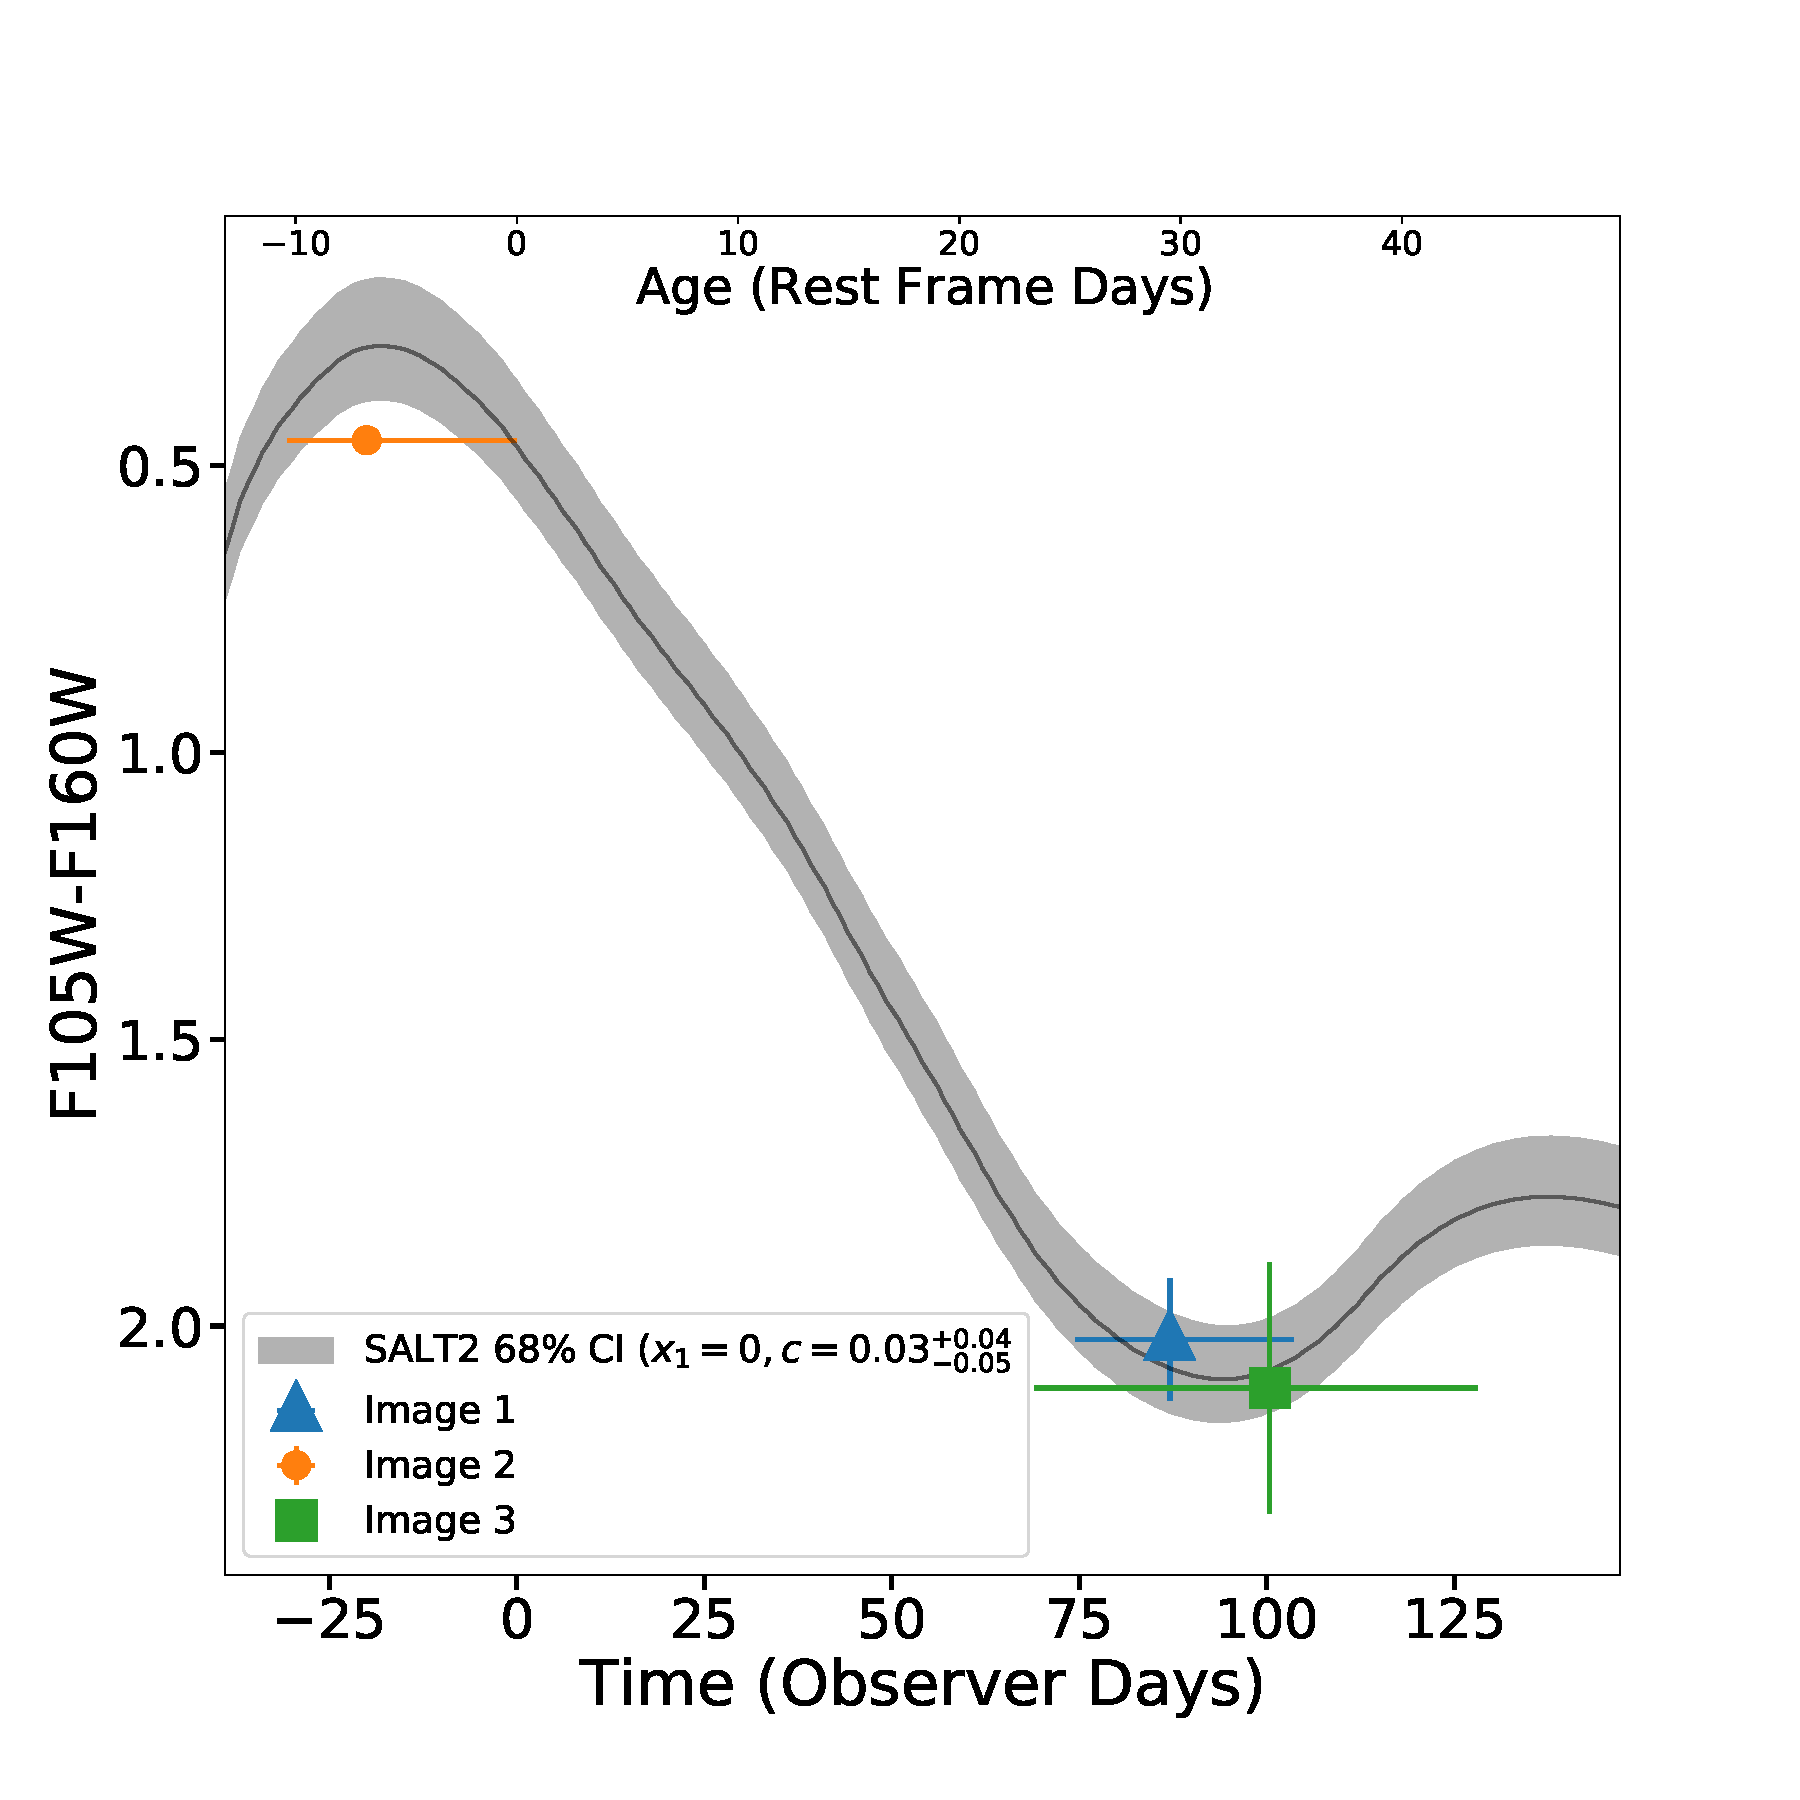
\includegraphics[width=0.6\textwidth]{Paper/Figures/full_colorcurve_total.pdf}
    \caption{\label{fig:full_colorcurve} The reconstructed color curve for \SNABC, using best-fit lensing parameters. The grey shaded region covers the 68\% confidence interval of the best-fit SALT2 color curve, with the median model shown as a solid line. Observed photometry is shown as colored markers.  No magnification correction is needed to set the vertical position of each observed point, so error bars in the y direction represent only photometric uncertainty. The horizontal position is defined by the best-fit time delays reported in Table~1 of the main text, with error bars 
    representing the uncertainty in the final inferred time delays. }
\end{figure}

\clearpage

\section*{Supplementary Material}

\subsection*{Supplementary Note: Comparison to Previous Lens Modeling}

\added[id=r1]{
Ref \cite{newman_resolving_2018} (hereafter N18) provides a detailed analysis of this cluster, including sophisticated modeling of the lens.  The N18 lens modeling also uses \lenstool, but has several important differences.  Most notably, N18 uses source-plane instead of image-plane optimization, incorporates pixel-level data as constraints, and provides source-plane reconstructions of the lensed galaxy that we identify as the SN host.  
For this work, we find the \lenstool image-plane optimisation to be more robust because it deals better with actual positional uncertainties.  We did not incorporate pixel-level flux data, because the \lenstool code can only use observed fluxes when doing source plane optimisation.   }

\setcounter{table}{0} %\renewcommand{\thetable}{\arabic{figure}}
\begin{table}[tbp]
    \captionsetup{name={Supplementary Table}}
    \centering
    \begin{tabular}{crrrrr}
    Image     & $\langle$ $\mu_{\rm SN}$ $\rangle$ & $\mu_{\rm opt,SN}$ & $\mu_{\rm opt,gal.pk.}$ & $\mu_{\rm gal.avg.}$ & $\mu_{\rm N18,gal.avg.}$\\
\hline 
        1 & 3.9$\pm$0.5 &  6.7 & 4.35 & 10.0 & 12.5$\pm$5.4 \\
        2 & 7.4$\pm$3   & 15.2 &  6.9 &  8.3 & 10.3$\pm$3.1 \\
        3 & 5$\pm$1     &  4.3 & 3.64 &  4.2 & 4.9$\pm$1.6 \\
    \end{tabular}
    \caption{
    \added[id=r1]{Comparison of magnification predictions with the N18 lens model.}
    }
    \label{tab:mu_comparison}
\end{table}

\added[id=r1]{
Table~\ref{tab:mu_comparison} shows the magnification values predicted by our lens model E in comparison to the values reported in N18. 
Column 2 repeats the magnifications given in the main text and Table~\ref{tab:massmodel}, which are the expectation values from the $\mu$ distributions generated by the \lenstool MCMC sampling over model parameter space.  Column 3 gives the ``optimized'' magnification, which is the $\mu$ value returned by the single model instance that has the minimum $\chi^2$ value (note that this may be significantly different from the peak of the $\mu$ distribution, as for image 2 in particular).  Both of these are magnifications for the location of each SN image. The fourth and fifth columns give magnification predictions for the SN host galaxy. Column 4 reports the minimum-$\chi^2$ magnification at the peak of the surface brightness profile for each galaxy image.  Column 5 reports the
ratio of the total flux to source flux of the host galaxy, which is effectively a flux-weighted harmonic mean of the magnification factors across each galaxy image. This last value is the most appropriate for comparison to the values of N18 (given in Column 6), which are computed in a similar way.  The uncertainties from N18 reflect an estimate of systematic uncertainties, derived from lens modeling variants. 

From the last two columns of Table~\ref{tab:mu_comparison} we see that our preferred lens model E magnifications are within 1$\sigma$ of the N18 model, though our predictions are systematically lower by about 20\%.  This agrees with the assessment of systematic uncertainties from our lens model variants discussed above, which are also shown as the asymmetric error bars on the SN magnitudes in Figure~\ref{fig:class}.  As seen in Figure~\ref{fig:class}c, a larger magnification value would make the SN {\it more} consistent with the expected luminosity of a Type Ia SN at this redshift---though it would also make it more consistent with some CC SN light curves, likely making the classification somewhat more ambiguous. 
We expect that new lens modeling of this cluster with alternate software and different choices of constraints will also be informative, and may improve on our model predictions.  
Both the N18 modeling and the construction of lens model E and our model variants are constructed blind (without knowledge of the SN magnitudes).
Future lens modeling could incorporate the measured magnitudes as constraints, potentially yielding a more robust prediction of the time delay for the fourth image. We hope that the discovery of \SNABC  will encourage such efforts.  
}



\subsection*{Supplementary Note: Future Work}


\subsubsection*{Future Lens Modeling}
\added[id=r1]{
The uncertainty in the predicted time delay from the lens model presented here is $\pm$540 days (in the observer frame).  Are there improvements to the lens modeling that could tighten this prediction?

Our lens modeling did not make use of the velocity dispersion of the BCG, measured as 390$\pm$10 km s$^{-1}$ from our MUSE data.  We did not have this measurement available prior to unblinding, and thus we have restricted ourselves to only consider fully blind lens models in this paper. However, future analyses could incorporate the BCG velocity dispersion and here we speculate about the impact.  With a preliminary extension of model E we find that the time delay predictions would likely shift by $<$15 days, and the predicted magnifications for SN images 1-3 would likely be larger by as much as $\sim$2.5$\times$.  This is within the range of our systematic uncertainty estimates based on lens models A-E.  We therefore expect that inclusion of the BCG velocity dispersion will not significantly impact the SN classification or time delay conclusions, but may improve the accuracy and precision of the time delay estimate for image SN4.  

One may anticipate that future observations of the lensing cluster (e.g. with JWST) will provide more lens modeling constraints, potentially including the discovery of new multiply-imaged systems and new redshift measurements. These would substantially improve the lens model time delay predictions. Application of different lens modeling approaches could also provide some added confidence that there are not systematic biases in the lens model time delay prediction.
}

\subsubsection*{Future Observations}
\added[id=r1]{
Though the $\pm540$ day time delay uncertainty is small relative to the baseline of $>7000$ days, it nevertheless represents a long period over which the field would need to be monitored for the reappearance.  Is it feasible to expect future observations to catch the reappearance of \SNABC close to peak brightness? 
Even if the time delay uncertainty remains on the order of $\pm1$ year, it would still be reasonable to execute a follow up campaign with a cadence of approximately 2 months. Since the SN is at a redshift of $z=1.95$, a span of, say, 50 days in the observer frame is 17 days in the rest frame, comparable to the rise-time of a Type Ia SN.  Thus, it is reasonable to expect that a relatively inexpensive monitoring campaign would be able to catch the return appearance of \SNABC at or before peak brightness, ensuring a well-sampled light curve for the final SN image.

If future follow-up observations are successful in capturing the full light curve of the final fourth image, then future lens modeling could also incorporate measured SN magnifications as constraints.  Measured magnifications from lensed Type Ia SNe have been used to test lens models at both the cluster and galaxy scale \cite{nordin_lensed_2014, rodney_illuminating_2015, dhawan_magnification_2020}.  The addition of astrometric constraints for the fourth image could also significantly improve the time delay predictions for a lens model \cite{birrer_astrometric_2019}---and this could be done even with a fully blinded analysis.  Measurement of the magnification for a lensed Type Ia SN can be done without adopting strong priors from a cosmological model \cite{patel_three_2014}, meaning that one can avoid a circular constraint when the \SNABC time delay is then used for cosmology.
}

\subsubsection*{Future Discoveries}
\added[id=r2]{
In addition to follow-up observations of \SNABC, we may also hope for more discoveries of similar cluster-lensed SNe with long time delays. The expected rate for such events is still highly uncertain, and published rate estimates to date can only be taken as extreme lower limits for the expected yield from future sky surveys \cite{riehm_near-ir_2011,li_rates_2012,petrushevska_searching_2018,petrushevska_strongly_2020}.  All of these past analyses have been 
limited to $\leq 5$ well-studied galaxy clusters.  Furthermore, they have only examined the set of {\it already known} multiply-imaged galaxies, and have 
explicitly predicted only the rate of events that would have a time delay of $<$5 years.  With these caveats, the predicted lower limits are of order 1 SN detection per year per cluster, for a deep survey with a detection limit of 27 AB mag \cite{li_rates_2012}.  At the $5\sigma$ limits of the Rubin Observatory ($i\sim23.4$ AB mag), the lower limit on that rate is reduced by about a factor of ten \cite{petrushevska_strongly_2020}. 

It is treacherous to extend these estimates to the larger population of all galaxy clusters that will be regularly observed by future wide-field surveys.  Nevertheless, let us make a crude extrapolation to motivate future work.  Consider the 1-year 2000 deg$^2$ High Latitude Survey (HLS) from the Roman Space Telescope \cite{spergel_wide_2015, troxel_synthetic_2021}, and let us conservatively apply the rate of 
$\sim$1~SN yr$^{-1}$ cluster$^{-1}$ to only the $\sim$10 most massive clusters in the HLS area. This still predicts at least 10 cluster-lensed SN detections, which is comparable to the few dozen galaxy-lensed SNe expected from the Roman SN cosmology survey \cite{pierel_projected_2020}.  
Similarly, if we apply the 10$\times$ lower rate for the Rubin Observatory to the most massive clusters in the LSST survey area, we would anticipate at least $\sim$10 detections over the 10-year survey.  

We hope that the discovery of \SNABC will motivate an improvement over this very rough estimation of future rates.   This would require a more complete census of lensing clusters, along with lens models to predict magnifications and time delays, and measurements of star formation and stellar mass in lensed galaxies to predict the SN explosion rates.   }

\clearpage

%Using Biblatex for the bibliography
%\printbibliography

%Using bibtex for the bibliography:
%\section*{References}
\bibliographystyle{naturemag}
%\bibliography{zotero_references}
\bibliography{references}

{\bf Data Availability Statement:} All HST images used in this work are available from the Mikulski Archive for Space Telescopes (mast.stsci.edu). All VLT MUSE spectroscopic data used in this work are available from  the ESO Archive Science Portal (archive.eso.org). The authors declare that all other data supporting the findings of this study (photometry, lens model inputs, etc.) are available within the paper and its supplementary information files.  All software tools used for primary analysis tasks are publicly available, as indicated in the text.


Correspondence and requests for materials may be addressed to S.R. (\href{mailto:srodney@sc.edu}{srodney@sc.edu}).

%%%%%%%%%%%% Acknowledgents
\section*{Acknowledgments}

Based on observations made with the NASA/ESA Hubble Space Telescope, obtained from the data archive at the Space Telescope Science Institute, and on observations collected at the European Organisation for Astronomical Research in the Southern Hemisphere under ESO programme 0103.A-0777(A).  
{\bf Funding:} Support for this work was provided by NASA through grant numbers HST-GO-14622, HST-GO-15663 and HST-AR-15050 from the Space Telescope Science Institute, which is operated by the Association of Universities for Research in Astronomy, Inc. under NASA contract NAS 5-26555.  The Cosmic Dawn Center of Excellence is funded by the Danish National Research Foundation under grant No. 140. M.A.\ and J.D.R.P.\ were supported by NASA Headquarters under the NASA Future Investigators in Earth and Space Science and Technology (FINESST) awards 80NSSC19K1414 and 80NSSC19K1418, respectively.  K.E.W.\ wishes to acknowledge funding from the Alfred P. Sloan Foundation. 

{\bf Author Contributions:} 
Conceptualization, S.A.R., G.B., and S.T.; Methodology, S.A.R., J.D.R.P., J.R., and K.F.O.; Investigation, G.B., J.R., S.T., M.A., and K.E.W.; Writing - Original Draft, G.B.\ and S.T.; Writing - Review \& Editing, S.A.R., G.B., J.D.R.P., J.R., S.T., K.F.O., M.A., and K.E.W.; Visualization, S.A.R., G.B., J.D.R.P., J.R., K.F.O.; Supervision, S.A.R., G.B., S.T., and K.E.W.; Funding Acquisition, M.A.\ \& K.E.W.

{\bf Competing Interests:} All authors declare no competing interests.

\end{document}
















